% These are "magic" comments understood by the "TeXStudio" editor
% !TeX encoding = UTF-8
% !TeX TS-program = lualatex
% !TeX TXS-program:bibliography = biber
% Document title: ETSETB TFG LaTeX Template
% Version: 5.1
% Author: 2023 Orestes Mas Casals
% License: ETSETB TFG LaTeX Template by Orestes Mas is marked with CC0 1.0 Universal

\documentclass[a4paper,twoside,12pt]{report}

% Load auxiliary packages for various tasks
% Document title: ETSETB TFG LaTeX Template
% Version: 5.0
% Author: 2023 Orestes Mas Casals
% License: ETSETB TFG LaTeX Template by Orestes Mas is marked with CC0 1.0 Universal

%%%% TOOLS %%%%
\usepackage{lipsum}
\usepackage{etoolbox}   % <<< Provides some macros to compare text
\usepackage{iftex}      % <<< Detect TeX engine used to compile the document

%%%% MATH SETUP %%%%
\usepackage{mathtools}
\usepackage{amsmath}
\usepackage{amssymb}
\usepackage{braket}

%%%% INTERNATIONAL SYSTEM NOTATION FOR UNITS IN NUMBERS %%%%
\usepackage{siunitx}

%%%% FONTS SETUP %%%%
\iftutex   % True if compiling with Unicode engines (XeTeX/LuaTeX)
  \usepackage{fontspec}
  \usepackage[math-style=ISO,
    warnings-off={mathtools-colon, mathtools-overbracket},
  ]{unicode-math}
  %  This package is only a wrapper for the two packages libertinus-type1 (pdfLaTeX) and libertinus-otf (LuaLaTeX/XeLaTeX).
  %  The Libertinus fonts are similiar to Libertine and Biolinum, but come with math symbols. 
  \usepackage{libertinus}
  % Use DejaVu Mono for monospaced font
  \usepackage[
    mono=true,serif=false,sans=false,math=false,
    TT={Scale=0.80,FakeStretch=1.0}]{dejavu-otf}
\else    % True if compiling with 8-bit engines (LaTeX/pdfLaTeX)
  \usepackage[T1]{fontenc}
  %  This package is only a wrapper for the two packages libertinus-type1 (pdfLaTeX) and libertinus-otf (LuaLaTeX/XeLaTeX).
  %  The Libertinus fonts are similiar to Libertine and Biolinum, but come with math symbols. 
  \usepackage{libertinus,libertinust1math}
  % Use DejaVu Mono for monospaced font
  \usepackage[scaled=0.80]{DejaVuSansMono}
  % Some declarations for the Gantt diagram example
  \DeclareUnicodeCharacter{1D49}{\textsuperscript{e}} % "ᵉ" character
  \DeclareUnicodeCharacter{02B3}{\textsuperscript{r}} % "ʳ" character
  \DeclareUnicodeCharacter{1D52}{\textsuperscript{o}} % "ᵒ" character
\fi
\usepackage{microtype}

%%%% PAGE GEOMETRY %%%%
\usepackage{geometry}

%%%% PAGE STYLE %%%%%
\usepackage{fancyhdr}

%%%% PARAGRAPH STYLE %%%%
% Blank line between paragraphs instead of first line indenting
\usepackage{parskip}

%%%% TITLES STYLE %%%%
\usepackage{titlesec}

%%%% COLOR DEFINITIONS %%%%
\usepackage[svgnames]{xcolor}

%%%% TABLES %%%%
%\usepackage{array}
\usepackage{tabularx,booktabs,wrapfig}
\usepackage{enumitem}

%%%% ACRONYMS %%%%
\usepackage{acro}
% class `abbrev': abbreviations:
\DeclareAcronym{EU}{
  short = EU,
  long  = European Union,
  tag = abbrev
}

\DeclareAcronym{ETSETB}{
  short = ETSETB,
  long  = Escola Tècnica Superior d'Enginyeria de Telecomunicació de Barcelona,
  tag = abbrev
}

\DeclareAcronym{GREELEC}{
  short = GREELEC,
  long  = Grau en Enginyeria Electrònica de Telecomunicació,
  tag = abbrev
}

\DeclareAcronym{GEF}{
  short = GEF,
  long  = Grau en Enginyeria Física,
  tag = abbrev
}

\DeclareAcronym{VQE}{
  short = VQE,
  long  = Variational Quantum Eigensolver,
  tag = abbrev
}

\DeclareAcronym{DQS}{
  short = DQS,
  long  = Digital Quantum Simulation,
  tag = abbrev
}

\DeclareAcronym{AQS}{
  short = AQS,
  long  = Analog Quantum Simulation,
  tag = abbrev
}

\DeclareAcronym{MPS}{
  short = MPS,
  long  = Matrix Product States,
  tag = abbrev
}

\DeclareAcronym{PEPS}{
  short = PEPS,
  long  = Projected Entangled Pair States,
  tag = abbrev
}

\DeclareAcronym{FCI}{
  short = FCI,
  long  = Full Configuration Interaction,
  tag = abbrev
}

\DeclareAcronym{CCSD}{
  short = CCSD,
  long  = Coupled Cluster with Singles and Doubles,
  tag = abbrev
}

\DeclareAcronym{ADAPT-VQE}{
  short = ADAPT-VQE,
  long  = Adaptive Variational Quantum Eigensolver,
  tag = abbrev
}

\DeclareAcronym{QNG}{
  short = QNG,
  long  = Quantum Natural Gradient,
  tag = abbrev
}

\DeclareAcronym{GD}{
  short = GD,
  long  = Gradient Descent,
  tag = abbrev
}

\DeclareAcronym{NMomentum}{
  short = NMomentum,
  long  = Nesterov Momentum,
  tag = abbrev
}

\DeclareAcronym{RMSProp}{
  short = RMSProp,
  long  = Root Mean Square Propagation,
  tag = abbrev
}

\DeclareAcronym{Adagrad}{
  short = Adagrad,
  long  = Adaptive Gradient Algorithm,
  tag = abbrev
}

\DeclareAcronym{Adam}{
  short = Adam,
  long  = Adaptive Moment Estimation,
  tag = abbrev
}

\DeclareAcronym{NISQ}{
  short = NISQ,
  long  = Noisy Intermediate-Scale Quantum,
  tag = abbrev
}

\DeclareAcronym{GPU}{
  short = GPU,
  long  = Graphics Processing Unit,
  tag = abbrev
}

\DeclareAcronym{CPU}{
  short = CPU,
  long  = Central Processing Unit,
  tag = abbrev
}

\DeclareAcronym{UCCSD}{
  short = UCCSD,
  long  = Unitary Coupled Cluster with Singles and Doubles,
  tag = abbrev
}

\DeclareAcronym{HF}{
  short = HF,
  long  = Hartree-Fock,
  tag = abbrev
}



%%%% GRAPHICS %%%%
\usepackage{graphicx}
\usepackage{caption}        %
\usepackage{tikz}           % Generic vector graphics language
\usepackage{pgfgantt}       % Gantt diagrams. See "pgfgantt" manual for reference

%%%% ELECTRONIC CIRCUITS %%%%
\usepackage{circuitikz}

%%%% PLOTTING %%%%
\usepackage{pgfplots}

%%%% COLOR BOXES %%%%
\usepackage{tcolorbox}

%%%% BIBLIOGRAPHY (using biblatex) %%%%
\usepackage[section,numbib]{tocbibind}       % Makes bibliography appear in the Table of Contents
\usepackage[backend=biber,style=numeric,sorting=none]{biblatex}
\addbibresource{TFG.bib}

%%%% QUOTES %%%%
\usepackage{csquotes}

%%%% HYPERLINKS %%%%
\usepackage{hyperref}

%%%% ADDED %%%%%
\usepackage{varwidth}
\usepackage{float}
\usepackage[utf8]{inputenc}
\usepackage{listings}
\usepackage{eurosym}

% Document style definitions. GHANGE STYLES THERE.
% Document title: ETSETB TFG LaTeX Template
% Version: 5.0
% Author: 2023 Orestes Mas Casals
% License: ETSETB TFG LaTeX Template by Orestes Mas is marked with CC0 1.0 Universal

%%% COLORS
\definecolor[named]{ETSETBcopper}{RGB}{220,68,05}
\definecolor[named]{UPCblue}{RGB}{15,128,204}
\colorlet{DefaultColor}{SlateGray}
\colorlet{GRETSTcolor}{SteelBlue}
\colorlet{GREELECcolor}{SeaGreen}
\colorlet{GEFcolor}{SlateBlue}
% This color will change according to the Degree set.
\colorlet{DegreeColor}{ETSETBcopper}

%%% PAGE GEOMETRIES
% Geometry of cover page
\newgeometry{
  headheight=2cm,
  headsep=1cm,
  top=3cm,
  bottom=3cm,
  left=3.5cm,
  right=2.5cm,
  top=4.5cm,           % Allow space on the top for the logos
}
\savegeometry{cover}

% Geometry for main content pages
\newgeometry{%
  headheight=30pt,
  headsep=1cm,
  top=3.5cm,
  bottom=3.5cm,
  footskip=1.5cm,
  left=3cm,
  right=3cm,
  marginparwidth=20pt,
}
\savegeometry{main}

%%% Redefinition of various commands
%%% It must be done this way, because these styles are hardcoded into Book class
\makeatletter
\renewcommand{\tableofcontents}{%
  \chapter*{\contentsname%
    \@mkboth{\contentsname}{\contentsname}%
  }%
  \@starttoc{toc}%
}
\renewcommand{\listoffigures}{%
  \chapter*{\listfigurename%
    \@mkboth{\listfigurename}{\listfigurename}%
  }%
  \@starttoc{lof}%
}
\renewcommand{\listoftables}{%
  \chapter*{\listtablename%
    \@mkboth{\listtablename}{\listtablename}%
  }%
  \@starttoc{lot}%
}
\makeatother

%%% HEADER / FOOTER STYLES FOR VARIOUS DOCUMENTS PARTS

% "plain" page style is invoked always (unless changed by user) at the first page of each chapter
\fancypagestyle{plain}{
  \fancyhf{}
  \renewcommand\headrulewidth{0pt}
  \renewcommand\footrulewidth{0pt}
  \fancyfoot[C]{-- \thepage\ --}
}

% Front cover style
\fancypagestyle{frontcover}[plain]{%
  \fancyhf{}     % Empty current header and footer
  \fancyhead[L]{
\includegraphics[height=1.75cm]{img/logos/Logo_UPC_ETSETB_tight.pdf}}
  \fancyhead[R]{
\includegraphics[height=1.75cm]{img/logos/logo_telecos.png}}
  \renewcommand{\footrulewidth}{6pt}%
  \futurelet\TMPfootrule\def\footrule{{\color{gray!80}\TMPfootrule}}
}

% Main content style
\fancypagestyle{main}[plain]{%
  % Draw a line under the heading of every page EXCEPT on float pages or if they start with a figure
  \renewcommand\headrulewidth{\iftopfloat{0pt}{\iffloatpage{0pt}{1pt}}}
  \futurelet\TMPheadrule\def\headrule{{\color{gray!80}\TMPheadrule}}
  % 
  \renewcommand{\chaptermark}[1]{\markboth{\chaptername\ \thechapter{}. ##1}{}}
  \renewcommand{\sectionmark}[1]{\markright{\thesection\ - ##1}}
  \fancyhead[LE]{\scshape\leftmark}
  \fancyhead[RO]{\scshape\rightmark}%
}

%%% STYLE FOR CHAPTER TITLE
% Format of titles is:
% \titleformat
%   {command}
%   [shape]
%   {format}
%   {label}
%   {sep}
%   {before-code}
%   [after-code]
\titleformat
{\chapter}%
[display]        % The "display" shape puts the label in a separate paragraph
{\sffamily\normalsize\Huge\color{black}}% Format of the whole title
{\flushright\sffamily\normalsize\color{DegreeColor}\hrulefill\hspace{1ex}%
   \MakeUppercase{\chaptertitlename}\hspace{1ex}% 
   {\sffamily\fontsize{60}{60}\selectfont\thechapter}%
}% Label format - A line followed by a "Chapter" string and a large colored chapter number
{5 pt}% Vertical separator between the label and the title body
{\flushright\bfseries\LARGE}% Code preceding title body (title is LARGE bold and raggedleft)
[]% Code after the title body.

%%% STYLE FOR TABLES %%%
% Increase spacing between cell content and borders
\renewcommand{\arraystretch}{1.3}

%%% BIBLIOGRAPHY STYLE %%%
\ExecuteBibliographyOptions{  
  sorting=nyt,
}
% Enlarge separation between bibliography items
\setlength\bibitemsep{0.5\baselineskip}

%%% FIGURE's CAPTION STYLE %%%
\DeclareCaptionFont{blue}{\color{blue}}
\captionsetup{
  labelfont={blue,sf,bf},
  textfont=it,
}

%%% TIKZ/PGF DRAWING GLOBAL STYLES %%%
\usetikzlibrary{
  babel,  % DON'T EVER TRY TO REMOVE THAT IF YOU USE THE "babel" PACKAGE !!
  angles,calc,quotes,
  arrows.meta,positioning,shapes.misc,shapes.geometric,
  patterns,decorations.pathmorphing,decorations.markings,
}
\tikzset{
}

%%% PGFPLOTS SETTINGS %%%
\pgfplotsset{
  compat=1.18,       % Avoiding a warning
}

%%% GANTT DIAGRAMS GLOBAL STYLES %%%
\ganttset{
  progress label text = {\pgfmathprintnumber[precision=0, verbatim]{#1}\% \ifcase\doclanguage\or completa\or completa\else complete\fi}
}

%%% TCOLORBOX STYLES
\tcbuselibrary{skins,breakable,listingsutf8}

%%% HYPERREF OPTIONS %%%
\hypersetup{
  breaklinks=true,
  colorlinks=true,    % CHANGE TO "true" IF YOU WANT COLORED TEXT LINKS INSTEAD OF BEING SURROUNDED BY A BORDER.
%  hidelinks,          % UNCOMMENT IF YOU WANT TO REMOVE COLOR AND BORDER AROUND THE LINKS.
}


%%%%%%%%%%%%%%%%%%%%%%%%%%%%%%%%%%%%%%%%%%%%%%%%%%%%%%%%%%%%%%%%%%%%%%
%%%                                                                %%%
%%%              DADES DEL DOCUMENT / DOCUMENT DATA                %%%
%%%                                                                %%%
%%%%%%%%%%%%%%%%%%%%%%%%%%%%%%%%%%%%%%%%%%%%%%%%%%%%%%%%%%%%%%%%%%%%%%

%%% Please UNCOMMENT and/or provide suitable information to the macros below
%%% Si us plau, DESCOMENTEU i/o ompliu les macros següents amb la informació adient.

%%% Specify the document language
%%%   1: Catalan
%%%   2: Spanish
%%%   3: English
\newcommand{\doclanguage}{3}

% Set-up language and load language-related cover page macros
% Document title: ETSETB TFG LaTeX Template
% Version: 5.0
% Author: 2023 Orestes Mas Casals
% License: ETSETB TFG LaTeX Template by Orestes Mas is marked with CC0 1.0 Universal

%%%% TEMPLATE LANGUAGE MACROS %%%%

% Language selection based on the language variable defined above
\ifcase\doclanguage\or
  % Case 1
  \usepackage[catalan]{babel}
  \selectlanguage{catalan}%
  \setquotestyle{spanish}% El paquet "csquotes" no té estil pel català, però podem usar l'espanyol
  \newcommand\TFGdate{
    \ifcase\month\or%
      Gener\or Febrer\or Març\or Abril\or
      Maig\or Juny\or Juliol\or Agost\or
      Setembre\or Octubre\or Novembre\or Desembre\fi
      \space de~\number\year%
    }
\or % Case 2
  \usepackage[spanish,es-noquoting]{babel}
  \selectlanguage{spanish}%
  \newcommand\TFGdate{
    \ifcase\month\or%
      Enero\or Febrero\or Marzo\or Abril\or
      Mayo\or Junio\or Julio\or Agosto\or
      Septiembre\or Octubre\or Noviembre\or Diciembre\fi
      \space de~\number\year%
    }
\else % Case 3 (default)
  \usepackage[english]{babel}
  \selectlanguage{english}%
  \newcommand\TFGdate{
    \ifcase\month\or%
      January\or February\or March\or April\or
      May\or June\or July\or August\or
      September\or October\or November\or December\fi
      \space\number\year%
    }
\fi

\newcommand\degreename{
  \ifcase\doclanguage
  \or
    \{Nom del Grau\}%
  \or
    \{Nombre del Grado\}%
  \else
    \{Degree's Name\}%
  \fi
}

\newcommand\GEF{
  \ifcase\doclanguage
  \or
    Grau en Enginyeria Física
  \or
    Grado en Ingeniería Física
  \else
    Degree in Physics Engineering
  \fi
}

\newcommand\GRETST{
  \ifcase\doclanguage
  \or
    Grau en Enginyeria de Tecnologies i Serveis de Telecomunicació
  \or
    Grado en Ingeniería de Tecnologías y Servicios de Telecomunicación
  \else
    Degree in Telecommunication Technologies and Services Engineering
  \fi
}

\newcommand\GREELEC{
  \ifcase\doclanguage
  \or
    Grau en Enginyeria Electrònica de Telecomunicació
  \or
    Grado en Ingeniería Electrónica de Telecomunicación
  \else
    Degree in Electronics Engineering%  Should be "Degree in Telecommunication Electronics Engineering"
  \fi
}

\newcommand{\studentsname}{
  \ifcase\doclanguage
  \or
    \{Nom de l'Autor\}%
  \or
    \{Nombre del Autor\}%
  \else
    \{Author's Name\}%
  \fi
}

\newcommand\reporttitle{
  \ifcase\doclanguage
  \or
    \{Títol del Treball\}%
  \or
    \{Título del Trabajo\}%
  \else
    \{Report's title\}%
  \fi
}

\newcommand\FirstParagraph{
  \ifcase\doclanguage
  \or
    Treball de Fi de Grau\medskip\\
    presentat a l'Escola Tècnica Superior\medskip\\
    d'Enginyeria de Telecomunicació de Barcelona\medskip\\
    de la Universitat Politècnica de Catalunya\medskip\\
    per
  \or
    Trabajo de Final de Grado\medskip\\
    presentado en la Escola Tècnica Superior\medskip\\
    d'Enginyeria de Telecomunicació de Barcelona\medskip\\
    de la Universitat Politècnica de Catalunya\medskip\\
    por
  \else
    Bachelor's Degree Thesis\medskip\\
    Submitted to the Faculty at the\medskip\\
    Escola Tècnica Superior\medskip\\
    d'Enginyeria de Telecomunicació de Barcelona\medskip\\
    of the Universitat Politècnica de Catalunya\medskip\\
    by
  \fi
}

\newcommand\SecondParagraph{
  \ifcase\doclanguage
  \or
    En compliment parcial\medskip\\
    dels requisits per a l'obtenció del
  \or
    En cumplimiento parcial\medskip\\
    de los requisitos para la obtención del
  \else
    In partial fulfillment\medskip\\
    of the requirements for the
  \fi
}

\newcommand\advisor{
  \ifcase\doclanguage
  \or
    \textit{\{Nom del director del projecte\}}
  \or
    \textit{\{Nombre del director del proyecto\}}
  \else
    \textit{\{Advisor's Name\}}
  \fi
}

\newcommand\reviewer{
  \ifcase\doclanguage
  \or
    \textit{\{Nom del ponent (si s'escau)\}}
  \or
    \textit{\{Nombre del ponente (si aplica)\}}
  \else
    \textit{\{Reviewer's Name (if applicable)\}}
  \fi
}

\newcommand\ThesisTitle{\reporttitle}
\newcommand\AuthorName{\studentsname}
\newcommand\DegreeName{\degreename}
\newcommand\AdvisorName{\advisor}
\newcommand\ReviewerName{\reviewer}
\newcommand\documentDate{\TFGdate}
\newcommand\AdvisorLine{
  \ifcase\doclanguage
  \or
    Director/a:
  \or
    Director/a:
  \else
    Advisor:
  \fi \AdvisorName
}
\newcommand\ReviewerLine{
  \ifcase\doclanguage
  \or
    Ponent:
  \or
    Ponente:
  \else
    Reviewer:
  \fi \ReviewerName
}

% Define some macros for user-provided information
\newcommand\setTitle[1]{\renewcommand{\ThesisTitle}{#1}}
\newcommand\setAuthor[1]{\renewcommand{\AuthorName}{#1}}
\newcommand\setDegree[1]{%
  \renewcommand{\DegreeName}{#1}
  % This stablishes a different color for each Degree
  % It's only a proposal and proof-of-concept. By now it's disabled until approval
%  \ifdefstring{\DegreeName}{\GRETST}{
%    \colorlet{DegreeColor}{GRETSTcolor}
%  }{
%    \ifdefstring{\DegreeName}{\GREELEC}{
%      \colorlet{DegreeColor}{GREELECcolor}
%    }{
%      \ifdefstring{\DegreeName}{\GEF}{
%        \colorlet{DegreeColor}{GEFcolor}
%      }{
%        \colorlet{DegreeColor}{UPCblue}
%      }
%    }
%  }
}
\newcommand\setAdvisor[1]{\renewcommand{\AdvisorName}{#1}}
\newcommand\setReviewer[1]{\renewcommand{\ReviewerName}{#1}}
\newcommand\setDate[1]{\renewcommand{\documentDate}{#1}}



%%% Thesis Title / Títol del TFG
\setTitle{Quantum Simulation}

%%% Name of the Thesis Author / Nom de l'autor del TFG
\setAuthor{Albert López Escudero}

%%% Degree's name. Uncomment the "setDegree" macro and set its argument to one:
%%% Nom del Grau. Descomenteu la macro «setDegree» i passeu-li un d'aquests paràmetres:
%%%   \GEF     - Physics Engineering            <<<< DON'T USE THIS, as the template is not approved by the GEF faculty yet
%%%   \GREELEC - Electronics Engineering
%%%   \GRETST  - Telecommunications Engineering
\setDegree{\GREELEC}

%%% Name of the Thesis Advisor / Director
\setAdvisor{Vincenzo de Maio \& Ivona Bandric}

%%% Name of the Thesis Rewiewer / «Ponent»
\setReviewer{Javier Rodrigez Fonollosa}

%%% Document's date (\TFGdate by default)
\setDate{\TFGdate}


%%%%%%%%%%%%%%%%%%%%%%%%%%%%%%%%%%%%%%%%%%%%%%%%%%%%%%%%%%%%%%%%%%%%%%%%%%
%%%%%%%%%%%%%%%%%%%%% PREAMBLE ENDS - DOCUMENT BEGINS %%%%%%%%%%%%%%%%%%%%
%%%%%%%%%%%%%%%%%%%%%%%%%%%%%%%%%%%%%%%%%%%%%%%%%%%%%%%%%%%%%%%%%%%%%%%%%%

\begin{document}

%%%%%%%%%%%%%%%%%%%%%%%%% FRONT COVER %%%%%%%%%%%%%%%%%%%%%%%%%
\begin{titlepage}
  % Cover page style defined in config/styles.tex
  \loadgeometry{cover}
  \thispagestyle{frontcover}
  % Use a Sans Serif typeface throughout
  \sffamily
  
  % Title page background image
  \begin{tikzpicture}[remember picture,overlay]
    \node[anchor=center,opacity=0.3,xshift=5mm,yshift=-10mm,scale=8] (Campillo) at (current page.center) {
\includegraphics{img/Campillo.png}};
    \filldraw[color=DegreeColor] (current page.south west) rectangle +(1.5cm,\paperheight);
    \filldraw[color=ETSETBcopper] (current page.south west) -- ++(0,0.140\paperheight-10pt) -- ++(0.75cm,20pt) --   ++(0.75cm,-20pt) -- ++(0,-0.140\paperheight+10pt) -- cycle;
    % This commented out sentence is work-in-progress
    % \node[anchor=south,at=(current page.south west),xshift=0.75cm,yshift=0.5cm] {\rotatebox{90}{\textcolor{white}{\Huge\bfseries \raisebox{-3pt}{ETSETB}~~~~\LARGE\DegreeName}}};
    \node[anchor=south,at=(current page.south west),xshift=0.75cm,yshift=0.5cm] {\rotatebox{90}{\textcolor{white}{\Huge\bfseries \raisebox{0pt}{ETSETB} -- \LARGE\DegreeName}}};
  \end{tikzpicture}
  
  \begin{center}
    \vspace*{2.5cm}
    
    {\Huge \ThesisTitle}\\
    
    \vspace{0.8cm}
    
    \color{black}\hrule height 2pt
    
    \vspace{1cm}
    
    {\large \FirstParagraph}\bigskip\\
  
    {\Large \AuthorName}\medskip\\
    
    \vspace{2.5cm}
    
    \SecondParagraph\medskip\\
    
    {\bfseries\scshape\DegreeName}
    
    % This is an elastic space
    \vfill
    
    \AdvisorLine\medskip\\
    
    %%% Comment out / delete the following line if there's no thesis reviewer
    \ReviewerLine\medskip\\
    
    \vspace{1cm}
    
    {Barcelona, \documentDate}
    
    \vspace{1cm}
  \end{center}
\end{titlepage}

% Restore default page geometry (modified by cover page code)
%\restoregeometry
\loadgeometry{main}

%%%%%%%%%%%%%%%%%%%%%%%%% PREAMBLE BEGINS %%%%%%%%%%%%%%%%%%%%%%%%%
\pagestyle{plain}


%%%% SUMMARY / RESUM %%%%
% DON'T CHANGE THIS LINE
\addcontentsline{toc}{section}{\ifcase\doclanguage\or Resum \or Resumen \else Summary\fi}

%%%% PLEASE REPLACE TEXTS WITH YOUR OWN CONTENT %%%%

%%% RESUM EN CATALÀ
\begin{center}
  \huge\bfseries\raggedright Resum~\hrulefill
\end{center}
  Cada exemplar del Treball de Fi de Grau (TFG) ha de contenir un Resum, que és un breu extracte del TFG. En termes d'estil, el Resum hauria de ser una versió reduïda del projecte: una introducció concisa, un compendi dels resultats i les principals conclusions o arguments presentats en el projecte. El Resum no ha de superar les 150 paraules i cal que estigui traduït al català, castellà i anglès.

%%% RESUMEN EN CASTELLANO
\begin{center}
  \huge\bfseries\raggedleft\vspace*{.5\baselineskip} \hrulefill ~Resumen
\end{center}
  Cada ejemplar del Trabajo de Fin de Grado (TFG) debe incluir un Resumenque es un breve extracto del TFG. En cuanto al estilo, el Resumen debería ser una versión reducida del proyecto: una introducción breve, un resumen de los resultados principales y las conclusiones o argumentos principales presentados en el proyecto. El Resumen no debe exceder las 150 palabras y debe estar traducido al catalán, castellano e inglés.

%%% ENGLISH SUMMARY
\begin{center}
  \huge\bfseries\raggedright\vspace*{.5\baselineskip} Summary~\hrulefill
\end{center}
  Each copy of the Bachelor's Thesis (TFG) must include a Summary, which is a concise abstract of the TFG. In terms of style, the Summary should be a condensed version of the project: a brief introduction, a summary of the main results, and the conclusions or key arguments presented in the project. The Summary should not exceed 150 words and must be translated to catalan, spanish and english.
                   % <<<<<< Please replace "summary.tex" entirely with your own content written in the required languages.


%%%% DEDICATION PAGE / PÀGINA DE DEDICATÒRIA %%%%
\clearpage
\thispagestyle{empty}             % No header/footer
\vspace*{4cm}                     % 
\hfill                            % Push the minipage to the right
\begin{minipage}{0.8\textwidth}   % You can adjust the minipage width
  \raggedleft\itshape             % Text in italics and flushed to the right
  \ifcase\doclanguage\or          % REPLACE FROM HERE (including the \ifcase structure) WITH YOUR OWN TEXT
    Podeu incloure una pàgina de Dedicatòries just abans de la pàgina d’Agraïments, però no és un requisit.\or
    Puede incluirse una página de Dedicatorias justo antes de la página de Agradecimientos, pero no es un requisito.\else
    A Dedication page may be included in your thesis just before the Acknowledgments page, but it is not a requirement.\fi
\end{minipage}



%%%% ACKNOWLEDGEMENTS / AGRAÏMENTS %%%%
\clearpage
\ifcase\doclanguage    % REPLACE FROM HERE (including the \ifcase structure) WITH YOUR OWN TEXT
\or
\chapter*{Agraïments}
\addcontentsline{toc}{section}{Agraïments}

És apropiat, però no obligatori, declarar l’extensió de l’ajuda aportada per persones de l'\textit{staff}, companys/companyes d’estudis, tècnics/ques o altres en la co\l.lecció de dades, disseny i construcció del prototip, l’anàlisi de dades, l’execució dels experiments i la preparació del projecte (incloent l’ajuda editorial). A més a més, és apropiat reconèixer la supervisió i la direcció donada pel tutor/a.
\or
\chapter*{Agradecimientos}
\addcontentsline{toc}{section}{Agradecimientos}

Es apropiado, aunque no obligatorio, declarar la extensión de la ayuda recibida por personas del staff, compañeros/as estudios, técnicos/as u otras en la recolección de datos, preparación del proyecto (incluyendo ayuda editorial). Además, es apropiado reconocer la supervisión, ayuda y dirección aportada por el tutor/a. 
\else
\chapter*{Acknowledgements}
\addcontentsline{toc}{section}{Acknowledgements}

It is appropriate, but not mandatory, to declare the extent to which assistance has been given by members of the staff, fellow students, technicians or others in the collection of materials and data, the design and construction of apparatus, the performance of experiments, the analysis of data, and the preparation of the thesis (including editorial help). In addition, it is appropriate to recognize the supervision and advice given by your advisor.
\fi



%%%% REVISION HISTORY TABLE %%%% <<<<<< Please read the instructions inside the "revision_history.tex" file.
\vspace*{0cm}

% As the Revision History has three LaTeX tables, in this particular case it's better to separate the translations in three different files.
% Please modify the one that suit your needs and this code will ignore the languages you're not working on.

\ifcase\doclanguage\or
  \vspace*{0cm}

\chapter*{Historial de revisió i aprovació}
\addcontentsline{toc}{section}{Historial de revisió i aprovació}

\begin{tabularx}{\textwidth}{|c|l|l|X|}
  \hline
    \textbf{Revisió} & \textbf{Data} & \textbf{Autor(s)} & \textbf{Descripció} \\
  \hline
    1.0 & dd/mm/yyyy & AME & Creació del document \\
  \hline
    1.1 & dd/mm/yyyy & AME, JPV & Correcció d'errors \\
  \hline
    2.0 & dd/mm/yyyy & AME, MLO & Versió revisada \\
  \hline
    4.0 & dd/mm/yyyy & AME & Versió final \\
  \hline
    & & & \\
  \hline
\end{tabularx}

\vspace{1cm}

\textbf{LLISTA DE DISTRIBUCIÓ DEL DOCUMENT}

\begin{tabularx}{\textwidth}{|l|X|}
  \hline
    \textbf{Rol} & \textbf{Cognom(s) i Nom} \\
  \hline
    [Estudiant] &  \\
  \hline
    [Director del projecte] &  \\
  \hline
    [Director 2 (si aplica)] &  \\
  \hline
\end{tabularx}

\vspace{1cm}

\begin{tabularx}{\textwidth}{|l|X||l|X|}
  \hline
    \multicolumn{2}{|l||}{\textbf{Escrit per:}}  &  \multicolumn{2}{l|}{\textbf{Revisat i aprovat per:}} \\
  \hline
    Data &  dd/mm/yyyy & Data &  dd/mm/yyyy \\
  \hline
    Nom &  Xxxxxxx Yyyyyyy & Nom &  Xxxxxxx Yyyyyyy \\
  \hline
    Rol & Autor del projecte & Rol & Director del projecte \\
  \hline
\end{tabularx}


\or
  \vspace*{0cm}

\chapter*{Historial de revisión y aprobación}
\addcontentsline{toc}{section}{Historial de revisión y aprobación}

\begin{tabularx}{\textwidth}{|c|l|l|X|}
  \hline
    \textbf{Revisión} & \textbf{Fecha} & \textbf{Autor(es)} & \textbf{Descripción} \\
  \hline
    1.0 & dd/mm/yyyy & AME & Creación del documento \\
  \hline
    1.1 & dd/mm/yyyy & AME, JPV & Corrección de errores \\
  \hline
    2.0 & dd/mm/yyyy & AME, MLO & Versión revisada \\
  \hline
    4.0 & dd/mm/yyyy & AME & Versión final \\
  \hline
    & & & \\
  \hline
\end{tabularx}

\vspace{1cm}

\textbf{LISTA DE DISTRIBUCIÓN DEL DOCUMENTO}

\begin{tabularx}{\textwidth}{|l|X|}
  \hline
    \textbf{Rol} & \textbf{Apellido(s) y Nombre} \\
  \hline
    [Estudiante] &  \\
  \hline
    [Director del proyecto] &  \\
  \hline
    [Director 2 (sólo si aplica)] &  \\
  \hline
\end{tabularx}

\vspace{1cm}

\begin{tabularx}{\textwidth}{|l|X||l|X|}
  \hline
    \multicolumn{2}{|l||}{\textbf{Escrito por:}}  &  \multicolumn{2}{l|}{\textbf{Revisado y aprobado por:}} \\
  \hline
    Fecha &  dd/mm/yyyy & Fecha &  dd/mm/yyyy \\
  \hline
    Nombre &  Albert López Escudero & Nombre &  Xxxxxxx Yyyyyyy \\
  \hline
    Rol & Autor del proyecto & Rol & Director del proyecto \\
  \hline
\end{tabularx}


\else
  \vspace*{0cm}

\chapter*{Revision history and approval record}
\addcontentsline{toc}{section}{Revision history and approval record}
  
\begin{tabularx}{\textwidth}{|c|l|l|X|}
  \hline
  \textbf{Revision} & \textbf{Date} & \textbf{Author(s)} & \textbf{Description} \\
  \hline
  1.0 & dd/mm/yyyy & AME & Document creation \\
  \hline
  1.1 & dd/mm/yyyy & AME, JPV & Error correction \\
  \hline
  2.0 & dd/mm/yyyy & AME, MLO & Revised after review \\
  \hline
  4.0 & dd/mm/yyyy & AME & Final version \\
  \hline
  & & & \\
  \hline
\end{tabularx}

\vspace{1cm}

\textbf{DOCUMENT DISTRIBUTION LIST}

\begin{tabularx}{\textwidth}{|l|X|}
  \hline
    \textbf{Role} & \textbf{Surname(s) and Name} \\
  \hline
    [Student] &  \\
  \hline
    [Project Supervisor 1] &  \\
  \hline
    [Project Supervisor 2 (if applicable)] &  \\
  \hline
\end{tabularx}

\vspace{1cm}

\begin{tabularx}{\textwidth}{|l|X||l|X|}
  \hline
    \multicolumn{2}{|l||}{\textbf{Written by:}}  &  \multicolumn{2}{l|}{\textbf{Reviewed and approved by:}} \\
  \hline
    Date &  dd/mm/yyyy & Date &  dd/mm/yyyy \\
  \hline
    Name &  Xxxxxxx Yyyyyyy & Name &  Xxxxxxx Yyyyyyy \\
  \hline
    Position & Project Author & Position & Project Supervisor \\
  \hline
\end{tabularx}

\fi


%%%% INDEX %%%%
\clearpage
\addcontentsline{toc}{section}{\ifcase\doclanguage\or Índex\or Índice\else Contents\fi}
\tableofcontents


%%%% LISTS %%%%
\listoffigures 
\addcontentsline{toc}{section}{\ifcase\doclanguage\or Índex de figures \or Lista de figuras \else List of figures\fi}
\listoftables
\addcontentsline{toc}{section}{\ifcase\doclanguage\or Índex de taules \or Índice de cuadros \else List of tables\fi}
%\lstlistoflistings


%%%% ACRONYMS %%%% <<<<<< PLEASE DEFINE YOUR ACRONYMS IN "acronyms.tex"
\clearpage
\newcommand\AbbrvName{\ifcase\doclanguage\or Sigles i acrònims\or Siglas y acrónimos\else Abbreviations\fi}
\addcontentsline{toc}{section}{\AbbrvName}
\printacronyms[
  heading=chapter*,
  display=all,
  include=abbrev,
  name=\AbbrvName,
]


%%%%%%%%%%%%%%%%%%%%%%%%%%%%%%%%%%%%%%%%%%%%%%%%%%%%%%%%%%%%%%%%%%%%
%%%%%%%%%%%%%%%%%%%%%%%%% MAIN PART BEGINS %%%%%%%%%%%%%%%%%%%%%%%%%
%%%%%%%%%%%%%%%%%%%%%%%%%%%%%%%%%%%%%%%%%%%%%%%%%%%%%%%%%%%%%%%%%%%%

% Starts normal numbering for the rest of the document
%\mainmatter  (valid/useful only if using the "book" class instead of "report" in the very first line)
\pagestyle{main}


% Introduction. Please replace "introduction.tex" entirely with your own content written in the desired language.
%%%% PLEASE REPLACE ENTIRELY WITH YOUR OWN CONTENT %%%%

\chapter{Introduction}


An Introduction that clearly states the rationale of the thesis that includes:


\begin{enumerate}

  \item Statement of purpose (objectives).

  \item Requirements and specifications.

  \item Methods and procedures, citing if this work is a continuation of another project or it uses applications, algorithms, software or hardware previously developed by other authors.
  
  \item Work plan with tasks, milestones and a Gantt diagram.

  \item Description of the deviations from the initial plan and incidences that may have occurred.
\end{enumerate}
The minimum chapters that this thesis document should have are described below, nevertheless they can have different names and more chapters can be added.

\section{Work goals}
The primary objective of this project is to contribute a new methodology to the realm of molecular simulations by:

\begin{itemize} \item Developing a quantum simulation program capable of efficiently modeling molecules using quantum algorithms. \item Introducing innovative code that implements adaptive circuit construction and advanced optimization strategies. \item Demonstrating the effectiveness of our approach by simulating selected molecular systems and comparing the results with classical computational methods. \item Enhancing the integration between quantum and classical computations to optimize both electronic and nuclear degrees of freedom. \end{itemize}

\section{Requirements and specifications}

To achieve these objectives, the following requirements and specifications have been established:

\begin{itemize} \item \textbf{Quantum Computing Frameworks}: Utilize quantum computing libraries such as PennyLane and JAX for quantum circuit simulation and automatic differentiation. \item \textbf{Algorithm Implementation}: Implement the VQE algorithm with adaptive circuit construction, allowing the selection of the most significant excitations based on energy gradients. \item \textbf{Optimization Techniques}: Employ efficient optimizers, including gradient-based methods like gradient descent and advanced techniques like the Quantum Natural Gradient optimizer. \item \textbf{Hamiltonian Construction}: Accurately build molecular Hamiltonians for various molecular geometries and ensure compatibility with standard quantum chemistry basis sets. \item \textbf{Visualization Tools}: Develop modules for visualizing energy convergence, parameter evolution, and molecular geometries throughout the optimization process. \item \textbf{Computational Resources}: Ensure the code is optimized for performance, making effective use of computational resources and supporting parallel execution where possible. \item \textbf{Extensibility}: Design the codebase to be modular and extensible, allowing future enhancements and adaptation to other molecular systems or quantum algorithms. \end{itemize}

\section{Methods and procedures}

This project introduces innovative methods and procedures to enhance molecular simulations using quantum computing. The key innovations in our code are centered around adaptive circuit construction, advanced optimization strategies, and the seamless integration of quantum and classical computations.

\subsection*{Adaptive Circuit Construction}

Traditional VQE implementations often rely on fixed ansätze, which may not efficiently capture the complexities of all molecular systems. Our code implements an adaptive approach where the quantum circuit is dynamically constructed by selecting excitations (operators) from a predefined pool based on their contribution to lowering the system's energy. This selection is guided by computing the energy gradients with respect to each operator, ensuring that only the most impactful excitations are included in the circuit. This method enhances computational efficiency and can lead to faster convergence to the ground state energy.

\subsection*{Advanced Optimization Techniques}

Optimizing the parameters of the quantum circuit is crucial for the success of the VQE algorithm. Our implementation leverages both gradient-based and gradient-free optimization methods. We utilize optimizers like the \textit{Gradient Descent Optimizer} and explore advanced techniques such as the \textit{Quantum Natural Gradient} optimizer, which accounts for the geometry of the parameter space and can provide faster convergence. Additionally, our code extends the optimization process to include the nuclear coordinates, allowing simultaneous optimization of the electronic structure and molecular geometry.

\subsection*{Integration of Quantum and Classical Computation}

Our code exemplifies a robust integration of quantum and classical computational techniques. By employing automatic differentiation tools provided by frameworks like JAX and PennyLane, we can efficiently compute gradients of the energy with respect to both circuit parameters and nuclear coordinates. This integration facilitates the optimization process and enables the handling of complex systems that are challenging for classical methods alone.

\subsection*{Innovations in Code Implementation}

Key innovations in our code include:

\begin{itemize} \item \textbf{Dynamic Operator Selection}: A procedure to compute energy gradients for each operator in the pool and select the one with the highest impact, thus adaptively constructing the quantum circuit. \item \textbf{Hybrid Optimization Loop}: An iterative loop that updates both quantum circuit parameters and nuclear positions, enhancing the ability to find the global minimum energy configuration. \item \textbf{Efficient Gradient Computation}: Implementation of numerical methods to compute gradients with respect to nuclear coordinates, enabling geometry optimization within the VQE framework. \item \textbf{Visualization and Analysis Tools}: Development of comprehensive visualization functions to analyze the optimization process, including energy evolution plots and 3D representations of molecular geometries. \item \textbf{Modularity and Extensibility}: A modular code structure that allows for easy adaptation to different molecules, basis sets, and quantum devices, facilitating future research and development. \end{itemize}

\subsection*{Utilization of Existing Frameworks and Contribution to the Field}

While our work builds upon established quantum computing frameworks such as PennyLane and utilizes existing algorithms like the VQE, the innovations introduced in our code represent significant advancements in the field of molecular simulations. By enhancing the efficiency of quantum simulations and providing new methods for adaptive circuit construction and parameter optimization, this project contributes valuable tools and methodologies to researchers and practitioners in quantum chemistry and quantum computing.

\section{Work plan}

  \label{sec:workplan}

Normally the figures and tables are put in \verb|\figure| and \verb|\table| environments, that can float freely in the document. You can identify each float with a \verb|\label|

\begin{figure}[H]
  \centering
  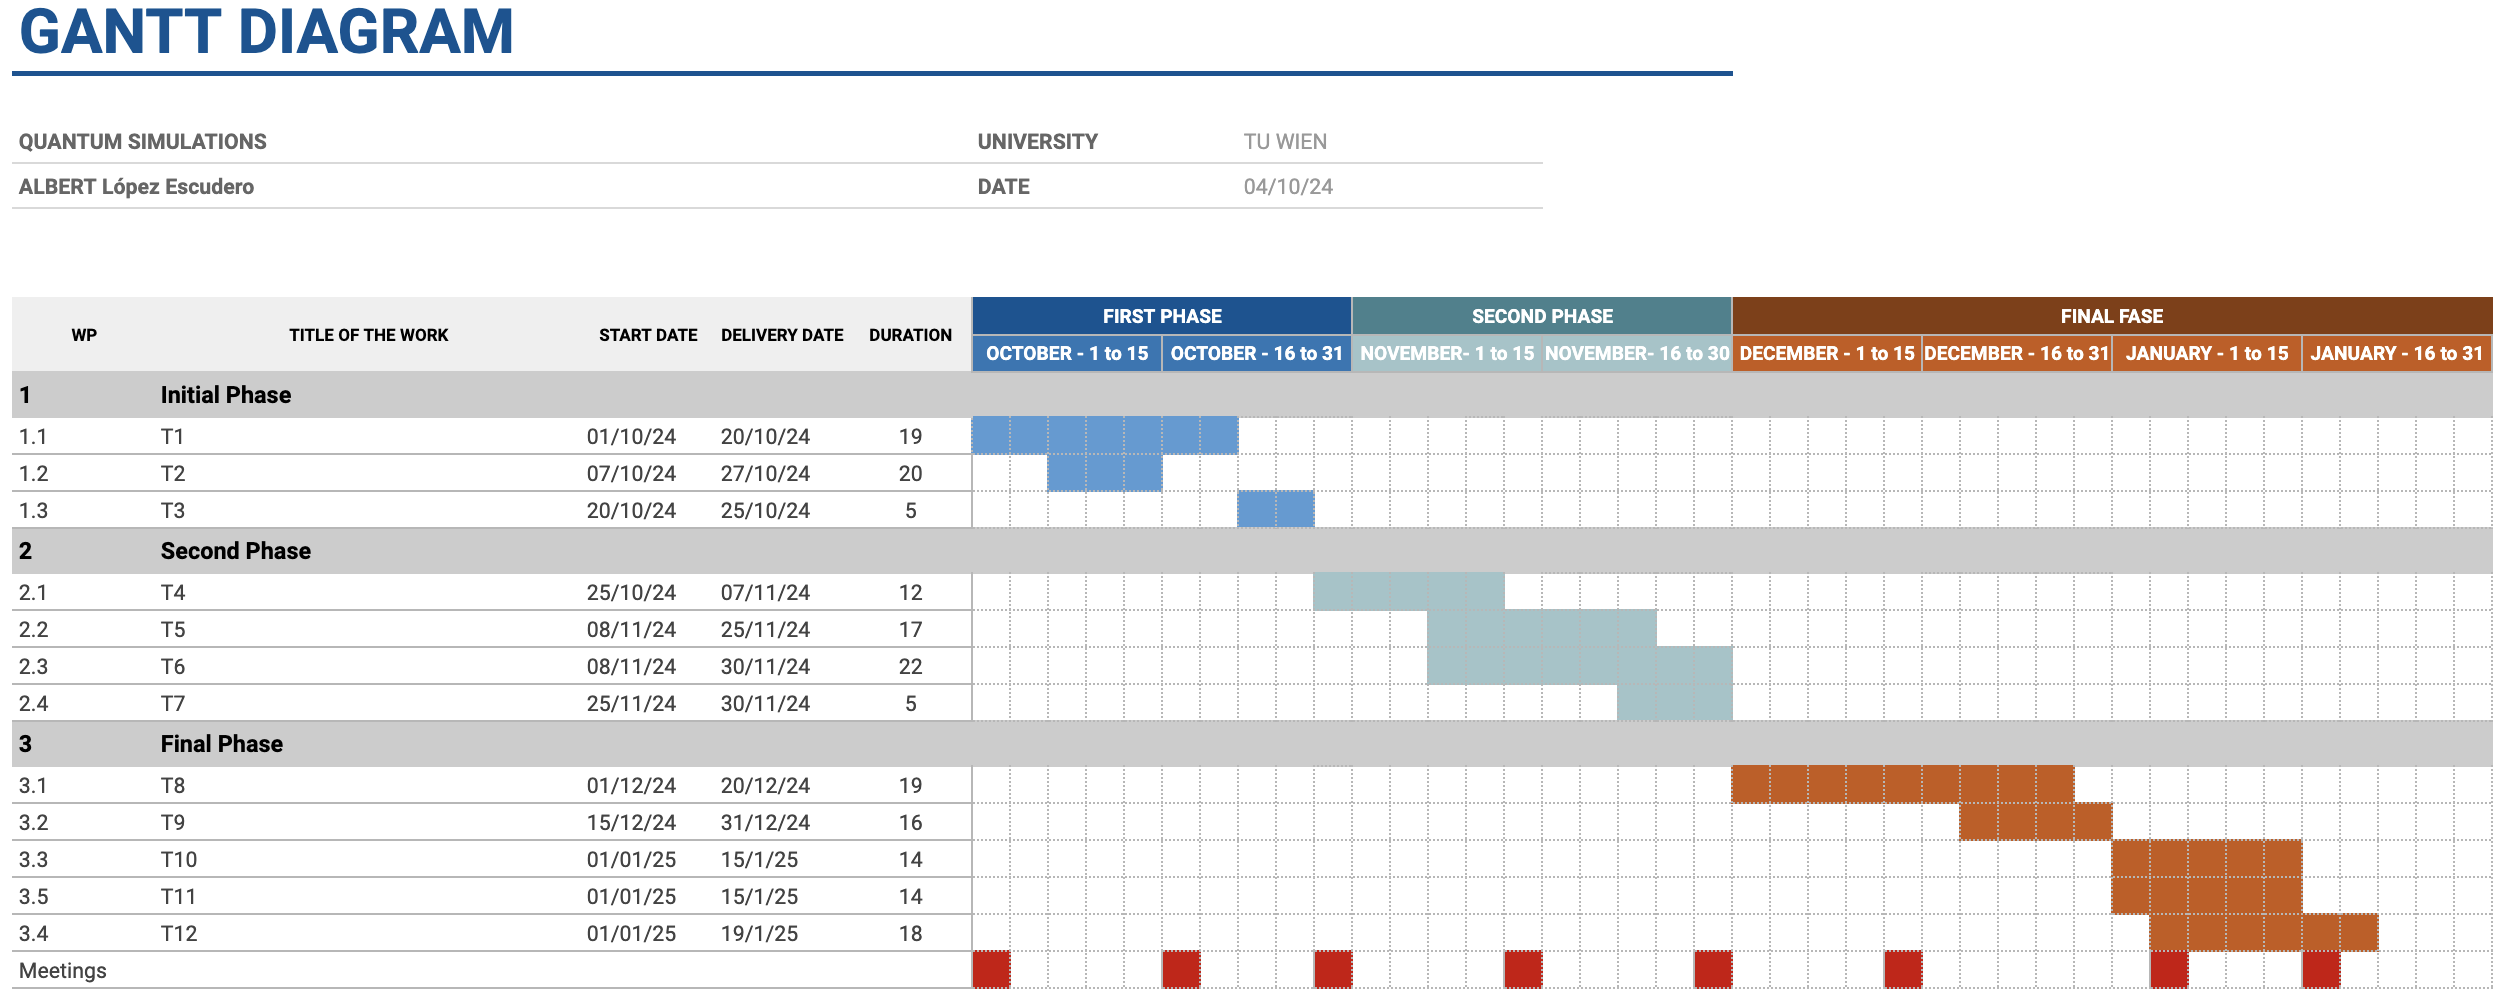
\includegraphics[width=1\textwidth]{img/Gantt_diagram.png}
  \caption{Project's Gantt diagram{\footnotesize{Gantt diagram of the project. For more information read the manual \cite{skalagantt} of Skala.}.}}
  \label{fig:gantt_diagram}
\end{figure}




% State of the art chapter. Please replace "state_of_art.tex" entirely with your own content written in the desired language.
\chapter[State of the Art]{State of the Art of the Technology Used or Applied in this Thesis}

In this project, we focus on the operation of quantum simulators applied to molecular simulation, an area where quantum computing offers significant advantages. The main objective is to develop a program capable of simulating different molecules in a simple and efficient manner.

To this end, we will review the basic concepts of quantum mechanics that are essential to understand the fundamentals and potential of quantum computing, and explore the techniques of quantum simulation that allow us to harness quantum computing capabilities even with current technological limitations.

\section{Quantum Simulation}

Quantum simulation has emerged as an advanced and essential technique for studying complex quantum systems, especially those that are inaccessible or present great challenges for direct analysis using classical methods. Based on the proposal of Richard Feynman, who postulated that a computer built from quantum elements could overcome the limitations of classical computers in simulating quantum phenomena, quantum simulation has progressed significantly. It encompasses both digital and analog simulations and has expanded its applicability in various scientific areas.

There are mainly two approaches in quantum simulation: \textbf{Digital Quantum Simulation (DQS)} and \textbf{Analog Quantum Simulation (AQS)}. DQS employs the quantum circuit model, where systems are represented by qubits that evolve through quantum gates to reproduce the dynamics of the target system. This approach is universal, as it can, in principle, simulate any quantum system, although not always efficiently. On the other hand, AQS involves creating a quantum system that directly emulates the Hamiltonian of the system under study, allowing certain properties of the simulated system, such as time evolution, to be reproduced approximately. This method is particularly useful when a qualitative representation is required rather than high precision.

In addition to these approaches, there are algorithms inspired by quantum information theory that facilitate the classical simulation of quantum systems. Techniques such as \textbf{Matrix Product States (MPS)} and \textbf{Projected Entangled Pair States (PEPS)} allow representing particle systems on classical computers more efficiently than standard classical methods, optimizing the calculation of properties of complex quantum systems.

The applications of quantum simulation are broad and encompass multiple scientific fields. In condensed matter physics, it allows the study of models such as the Hubbard model and quantum phase transitions, fundamental for understanding phenomena like superconductivity. In quantum chemistry, it facilitates the calculation of molecular energies and complex chemical reactions. In high-energy physics and cosmology, it emulates particles in high-energy fields and cosmological phenomena. Furthermore, quantum simulation is instrumental in the analysis of open quantum systems and in the investigation of quantum chaos, allowing exploration of interactions with the environment and chaotic dynamics in the quantum realm.

However, quantum simulation faces significant challenges related to the precise control of the quantum simulator systems and the management of decoherence and errors, which can affect the accuracy of the results. The amount of required resources, such as the number of qubits and quantum gates, also depends on the size and complexity of the system to be simulated. It is estimated that quantum simulators require between 40 and 100 qubits to surpass the computational power of classical computers in specific problems. Despite these challenges, technological advances continue to improve the viability and efficiency of quantum simulation, promising to transform research in natural sciences and expand our understanding of quantum phenomena.

\section{Key Concepts in Quantum Mechanics}

It is essential to understand the difference between bits in classical computing and qubits in quantum computing to delve into this new technological paradigm.

In classical computing, the basic unit of information is the \textbf{bit}, which can take the value of 0 or 1. These bits are the foundation upon which conventional computers operate, processing information through combinations of these binary states.

In contrast, quantum computing uses the \textbf{qubit} or quantum bit as its basic unit. Unlike the classical bit, a qubit can exist in a superposition of states, meaning it can simultaneously represent the values 0 and 1 thanks to the principle of superposition in quantum mechanics. This property, along with phenomena such as quantum entanglement and interference, allows quantum computers to process information exponentially more efficiently for certain problems.

\begin{figure}[H]
    \centering
    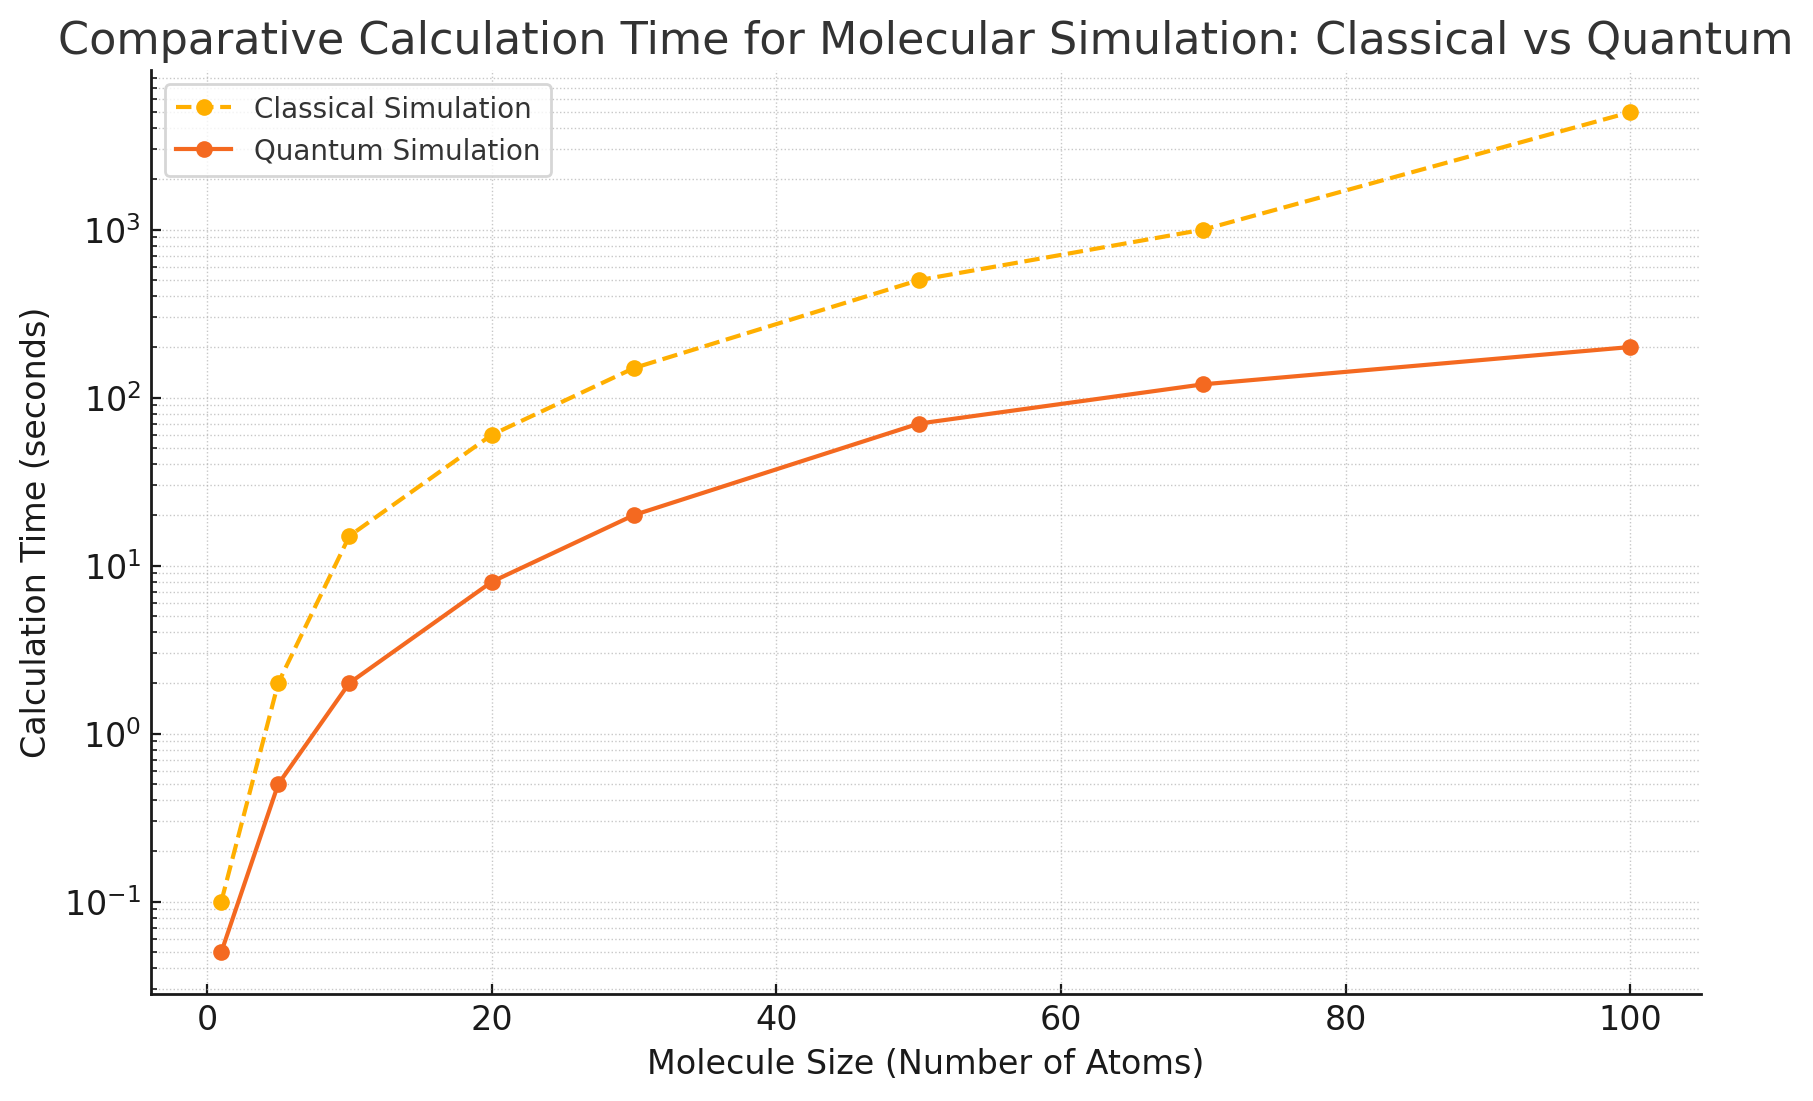
\includegraphics[width=0.8\textwidth]{img/bit_vs_qbit.png}
    \caption{Comparison of computation time for molecular simulations: classical vs quantum.}
    \label{fig:bit_vs_qubit}
\end{figure}

Understanding how qubits operate and their differences from classical bits is essential to appreciate the revolutionary potential of quantum computing.

\subsection{Qubit}

The \textbf{qubit} is the basic unit of information in quantum computing. While the classical bit can only be in one of two states (0 or 1), a qubit can be in a superposition of both states simultaneously. This is due to the principle of quantum superposition, one of the fundamental characteristics of quantum mechanics.

Mathematically, a qubit is represented as a linear combination of the basis states $\ket{0}$ and $\ket{1}$:

\[
\ket{\psi} = \alpha\ket{0} + \beta\ket{1}
\]

where $\alpha$ and $\beta$ are complex numbers that satisfy the normalization condition $|\alpha|^2 + |\beta|^2 = 1$. These coefficients indicate the probability amplitudes of finding the qubit in the states $\ket{0}$ or $\ket{1}$ upon measurement.

In addition to superposition, qubits can exhibit \textbf{quantum entanglement}, a property that allows creating strong correlations between qubits that cannot be explained by classical physics. Entanglement is essential for the computational power of quantum computers, as it enables processing and storing an exponentially larger amount of information than classical systems.

For example, while a classical system of $n$ bits can represent one of $2^n$ possible state combinations, a quantum system of $n$ qubits can represent a superposition of all those combinations simultaneously. This capability is what allows quantum computers to tackle complex problems more efficiently.

However, manipulating and maintaining qubits is a significant technical challenge. Qubits are extremely sensitive and can be affected by interactions with the environment, leading to \textbf{quantum decoherence}. To minimize this effect and preserve quantum properties, it is necessary to keep systems in controlled conditions, such as very low temperatures, close to absolute zero.

\subsection{Quantum Superposition}

\textbf{Quantum superposition} allows a quantum system to exist in multiple states simultaneously until a measurement is performed. This characteristic is key to the functioning of quantum computers, as it enables processing a large amount of information in parallel.

In quantum systems, superposition is combined with \textbf{quantum interference}, where the probability amplitudes of states can reinforce or cancel each other out. This phenomenon is exploited in quantum algorithms to increase the probability of obtaining the correct result. For example, in Grover's algorithm, constructive interference amplifies the probability of the desired state, significantly improving the efficiency of searching for elements in an unsorted database.

Superposition is especially useful in simulating complex molecular systems. Quantum computers can naturally model the superpositions of electronic states in molecules, which is crucial for studying chemical reactions and molecular properties that are difficult to address with classical methods due to the exponential growth of computational resources required.

\subsection{Quantum Decoherence}

\textbf{Quantum decoherence} is one of the main challenges in quantum computing. It refers to the loss of a system's quantum properties, such as superposition and entanglement, due to unwanted interactions with the environment. This loss causes the quantum system to transition toward classical behavior, affecting the accuracy and reliability of quantum calculations.

Qubits are extremely sensitive to external disturbances, such as electromagnetic fluctuations, vibrations, and temperature changes. These interactions can cause quantum states to mix with those of the environment, leading to a loss of coherence that is irreversible and degrades the stored quantum information.

To mitigate the effects of decoherence, various strategies are implemented:

\begin{itemize}
    \item \textbf{System Isolation}: Designing physical systems that minimize unwanted interactions with the environment, using materials and techniques that protect qubits from external disturbances.
    \item \textbf{Quantum Error Correction}: Implementing error correction codes that allow detecting and correcting errors without directly measuring the qubit's state, thereby preserving quantum information.
    \item \textbf{Dynamic Control}: Applying techniques such as pulse refocusing and dynamic pulse sequences that actively compensate for disturbances and extend the coherence time of qubits.
\end{itemize}

Controlling and mitigating decoherence are essential for the advancement of quantum computing and its application in areas like molecular simulation, where the precision of calculations is fundamental.

\section{The Hamiltonian in Quantum Mechanics}

The Hamiltonian is a fundamental concept originating from classical mechanics, introduced by William Rowan Hamilton in 1833. Hamiltonian mechanics is a reformulation of classical mechanics that provides powerful tools for studying the dynamics of systems. The Hamiltonian function represents the total energy of the system, expressed in terms of generalized coordinates and momenta, and is given by the sum of the kinetic and potential energies.

In quantum mechanics, the \textbf{Hamiltonian operator} plays a central role in describing the energy and time evolution of quantum systems. It represents the total energy of the system, including both kinetic and potential energies, and is essential for formulating the Schrödinger equation.

\subsection{Mathematical Definition}

The Hamiltonian operator, commonly denoted as \( \hat{H} \), is a self-adjoint operator acting on the Hilbert space associated with the quantum system. For a single particle in one dimension, the Hamiltonian is expressed as:

\[
\hat{H} = \hat{T} + \hat{V}
\]

where:

\begin{itemize}
    \item \( \hat{T} \) is the kinetic energy operator.
    \item \( \hat{V} \) is the potential energy operator.
\end{itemize}

In terms of the position \( \hat{x} \) and momentum \( \hat{p} \) operators, these are defined as:

\[
\hat{T} = \frac{\hat{p}^2}{2m} = -\frac{\hbar^2}{2m} \frac{d^2}{dx^2}
\]

\[
\hat{V} = V(\hat{x})
\]

Here, \( m \) is the mass of the particle, \( \hbar \) is the reduced Planck constant, and \( V(\hat{x}) \) is the potential energy function depending on position.

\subsection{Role in the Schrödinger Equation}

The Hamiltonian is central to the Schrödinger equation, which describes how the quantum state of a system evolves over time. The time-dependent Schrödinger equation is expressed as:

\[
i\hbar \frac{\partial}{\partial t} |\psi(t)\rangle = \hat{H} |\psi(t)\rangle
\]

where \( |\psi(t)\rangle \) is the state vector of the system at time \( t \). For time-independent systems, the Schrödinger equation reduces to the eigenvalue equation:

\[
\hat{H} |\psi\rangle = E |\psi\rangle
\]

Here, \( E \) represents the eigenvalues of the Hamiltonian, corresponding to the allowed energy levels of the system, and \( |\psi\rangle \) are the associated eigenstates.

\subsection{Hamiltonian in Multi-Particle Systems}

For systems with multiple particles, the Hamiltonian includes additional terms representing interactions between particles. For example, for a system of two particles, the Hamiltonian is expressed as:

\[
\hat{H} = \hat{T}_1 + \hat{T}_2 + \hat{V}_1 + \hat{V}_2 + \hat{V}_{12}
\]

where:

\begin{itemize}
    \item \( \hat{T}_1 \) and \( \hat{T}_2 \) are the kinetic energy operators of particles 1 and 2, respectively.
    \item \( \hat{V}_1 \) and \( \hat{V}_2 \) are the individual potential energy operators.
    \item \( \hat{V}_{12} \) represents the potential interaction between the two particles.
\end{itemize}

\subsection{Importance in Quantum Simulations}

In quantum simulations, especially in algorithms like the Variational Quantum Eigensolver (VQE), the Hamiltonian is decomposed into a sum of simpler terms, often expressed in terms of Pauli operators. This decomposition facilitates implementation on quantum circuits and allows estimating the system's energy through measurements on qubits.

Understanding the structure and properties of the Hamiltonian is essential for modeling and simulating quantum systems, as it determines the possible energies and dynamics of the system under study.

\section{VQE: Variational Quantum Eigensolver}
\label{sec:vqe}

Among the hybrid quantum-classical algorithms developed to address quantum simulation challenges, the \emph{Variational Quantum Eigensolver (VQE)} has gained particular relevance. This method seeks to approximate the ground-state energy of a target Hamiltonian, such as the electronic Hamiltonian of a molecule, by efficiently combining quantum state preparation with classical optimization techniques.

\subsection{Fundamental Principles and Stages of the Algorithm}
\label{subsec:vqe_principles_stages}

VQE is founded on the \textbf{variational principle} of quantum mechanics, which states that the expectation value of the energy 
\(\,E(\vec{\theta})\)
for any normalized trial state \(\,\ket{\psi(\vec{\theta})}\) is always an upper bound to the true ground-state energy \(E_0\):
\[
E(\vec{\theta}) 
= \bra{\psi(\vec{\theta})} \hat{H} \ket{\psi(\vec{\theta})}
\;\;\geq\; E_0.
\]
Because \(E(\vec{\theta})\) depends on a set of parameters \(\vec{\theta}\), the VQE algorithm iteratively updates these parameters to minimize \(E(\vec{\theta})\). Once no further reduction in \(E(\vec{\theta})\) is possible, the algorithm identifies the lowest value reached as an approximation of \(E_0\).

In practice, VQE proceeds in a loop that integrates quantum and classical resources:

\begin{enumerate}
    \item \textbf{Quantum State Preparation:} 
    A parameterized quantum circuit, commonly termed an \emph{ansatz}, is constructed with a set of adjustable parameters \(\vec{\theta}\). This circuit leverages unitary gates (e.g., single-qubit rotations, entangling gates) to create a trial wavefunction:
    \[
    \ket{\psi(\vec{\theta})}.
    \]

    \item \textbf{Measurement of the Expected Energy:}
    The Hamiltonian \(\hat{H}\) is decomposed into a sum of Pauli operators acting on the qubits. The expectation value 
    \(\langle \psi(\vec{\theta}) \mid \hat{H} \mid \psi(\vec{\theta}) \rangle\)
    is obtained by measuring the appropriate Pauli operators on the quantum device, typically requiring multiple circuit executions due to non-commuting terms.

    \item \textbf{Classical Optimization:}
    The measured energy serves as a cost function, \(E(\vec{\theta})\). A classical optimizer---such as \emph{Gradient Descent} or \emph{Adam}---then updates the parameters \(\vec{\theta}\) to minimize this cost.

    \item \textbf{Iteration and Convergence:}
    Steps 1--3 repeat until a convergence criterion is satisfied, for instance,
    \[
    \left|\,E\bigl(\vec{\theta}_{k+1}\bigr) - E\bigl(\vec{\theta}_{k}\bigr)\right|
    \;<\;\delta,
    \]
    where \(\delta\) is a small threshold for energy differences. The final set \(\vec{\theta}^{*}\) yields an approximate ground-state wavefunction and energy.
\end{enumerate}

\subsection{Advantages and Challenges}
\label{subsec:vqe_challenges}

VQE has garnered extensive interest in fields like \textbf{quantum chemistry}, \textbf{materials science}, and even combinatorial optimization problems mapped to Hamiltonians. Its hybrid structure allows leveraging near-term quantum devices (with limited qubits and gate depths) while offloading resource-intensive tasks---such as parameter updates---to classical computers. 

Despite its promise, VQE faces several practical hurdles:

\begin{itemize}
    \item \textbf{Noise and Decoherence:} 
    Real quantum devices suffer from errors that deteriorate the fidelity of prepared states and measurements, requiring error-mitigation strategies and noise-aware ansatz designs.

    \item \textbf{Barren Plateaus:}
    High-dimensional parameter spaces can contain large regions where gradients vanish, complicating the search for global minima.

    \item \textbf{Measurement Overhead:}
    Decomposing a Hamiltonian into many Pauli terms demands running multiple circuits, increasing sampling time and exposure to hardware noise.

    \item \textbf{Circuit Depth:}
    Accurate ans\"atze for complex systems may require deep circuits that quickly exceed the coherence times of current quantum processors.
\end{itemize}

\subsection{Outlook in Quantum Simulation}
\label{subsec:vqe_outlook}

Continuous improvements in both hardware (qubit quality, gate fidelity, and error-correction schemes) and software (advanced ans\"atze, better optimizers, error mitigation) keep driving VQE toward practical applications. Recent strategies such as \emph{ADAPT-VQE}, which adaptively builds up an excitation operator set, and domain-specific ans\"atze integrated with error mitigation methods, further enhance VQE’s accuracy for molecular systems. 

As the number of qubits grows and quantum hardware matures, VQE is likely to become a central approach for tackling classically intractable problems in quantum chemistry, materials science, and beyond. Its flexible hybrid nature will continue to serve as a testbed for new optimization algorithms, ansatz designs, and measurement strategies, bridging current \emph{Noisy Intermediate-Scale Quantum (NISQ)} devices with the longer-term ambition of fault-tolerant quantum computing.

\section{Different Ans\"{a}tze in Quantum Chemistry and Quantum Computing}
In the context of variational quantum algorithms and quantum chemistry, an \textbf{ansatz} is a carefully chosen, often physically motivated, parametric form of the quantum state used to approximate the ground (or excited) state of a system described by a given Hamiltonian. The term \textit{ansatz} originates from the German word \textquotedblleft approach\textquotedblright\ or \textquotedblleft initial guess,\textquotedblright\ and it reflects the central idea that we propose a functional form (or circuit structure) for the wavefunction and then optimize the parameters in search of the lowest possible energy. 

Within the framework of the Variational Quantum Eigensolver (VQE), the ansatz is implemented as a parameterized quantum circuit whose gates depend on a set of continuous variables $\vec{\theta}$. By measuring the expectation value of the Hamiltonian with respect to this trial state, one obtains an energy estimate $E(\vec{\theta})$ which is then iteratively minimized by a classical optimizer. The success of a VQE calculation hinges critically on the expressiveness and resource requirements (number of gates, circuit depth, etc.) of the chosen ansatz.

Several ans\"{a}tze have been proposed to achieve a balance between accuracy and computational cost. Below, we summarize the most relevant approaches, highlighting their theoretical underpinnings and current usage in quantum simulation.

\subsection{Hartree--Fock-based Ans\"{a}tze (Classical Reference)}
A historically important \textquotedblleft classical\textquotedblright\ ansatz in quantum chemistry arises from the \textbf{Hartree--Fock (HF)} approximation. In this method, the total wavefunction is assumed to be a single Slater determinant constructed from one-particle orbitals. Although it captures the fundamental antisymmetry required by the Pauli exclusion principle (i.e., fermionic exchange), it neglects most of the electron correlation. Post-HF methods, such as Configuration Interaction (CI), Many-Body Perturbation Theory (MPn), and Coupled Cluster (CC), then build on this reference state by introducing additional terms that account for electron correlation.  

\begin{itemize}
    \item \textbf{Configuration Interaction (CI):} Expands the wavefunction in a basis of Slater determinants (excitations) beyond the HF reference. The Full CI approach is exact within the chosen basis but scales exponentially with system size. Truncated CI methods (CIS, CID, CISD, etc.) reduce the computational cost but still grow quickly with system size.

    \item \textbf{Coupled Cluster (CC):} Expresses the wavefunction via an exponential of excitation operators acting on the HF reference. Formally written as 
    \[
       |\Psi_{\mathrm{CC}}\rangle = e^{\hat{T}}|\Phi_{\mathrm{HF}}\rangle,
    \]
    where $\hat{T}$ is the sum of cluster excitation operators (singles, doubles, triples, etc.). Although Coupled Cluster with Singles and Doubles (CCSD) is often accurate, further inclusion of triples and higher excitations can be required for strongly correlated systems.
\end{itemize}

In the context of classical methods, these \textbf{ans\"{a}tze} serve as trial wavefunctions whose coefficients are optimized using high-performance classical algorithms. Their conceptual basis---constructing physically motivated trial states that capture crucial features of the system---carries over into quantum computing.

\subsection{Unitary Coupled Cluster (UCC)}
A key adaptation of the Coupled Cluster theory to quantum computing is the \textbf{Unitary Coupled Cluster (UCC)} ansatz. It modifies the standard CC exponential by making it explicitly unitary:

\[
|\Psi_{\mathrm{UCC}}\rangle 
= e^{\hat{T}(\vec{\theta}) - \hat{T}^\dagger(\vec{\theta})} \,|\Phi_{\mathrm{HF}}\rangle,
\]

where $\hat{T}(\vec{\theta})$ is typically truncated to include only single and double excitations (UCCSD). This approach guarantees that the resulting operator is unitary, which is crucial for hardware implementations in quantum computing since all gates must be unitary transformations. 

\begin{itemize}
    \item \textbf{UCCSD (Singles and Doubles):} The most widespread version of UCC is truncated at single and double excitations:
    \[
        \hat{T}(\vec{\theta}) = \sum_{i,a} \theta_{i}^{a} \hat{a}_a^\dagger \hat{a}_i 
          \,\,+\,\, 
          \sum_{i,j,a,b} \theta_{i,j}^{a,b} \hat{a}_a^\dagger \hat{a}_b^\dagger \hat{a}_j \hat{a}_i
          \,\,+\, \cdots
    \]
    Here, $i, j$ denote occupied orbitals and $a, b$ virtual (unoccupied) orbitals. By exponentiating both $\hat{T}$ and $\hat{T}^\dagger$, the wavefunction stays normalized. However, the circuit depth can become large since implementing the exponential of a sum of non-commuting operators requires a trotterization or related approximation.

    \item \textbf{ADAPT-VQE and Variants:} To mitigate the high circuit cost, variants like \textit{ADAPT-VQE} build up a UCC-type ansatz incrementally, selecting only those excitation operators that most significantly lower the energy at each step. This adaptive approach reduces the number of gates needed and often converges faster.
\end{itemize}

\subsection{Problem-Inspired or Custom Ans\"{a}tze}
In some cases, \textbf{custom ans\"{a}tze} are tailored to the specific physical or chemical system under investigation. For example, if certain symmetries (like particle number or spin) are known to be crucial for describing the ground state, one can design an ansatz that explicitly respects those symmetries. Such approaches can drastically reduce the parameter space and improve convergence, albeit with some additional effort in circuit design.

\section{Optimizers}
\label{sec:optimizers}

In quantum simulation algorithms such as the Variational Quantum Eigensolver (VQE), optimizers constitute a key element of the hybrid quantum-classical workflow. Their primary objective is to minimize the cost function
\[
E(\vec{\theta}) = \langle \psi(\vec{\theta}) \mid \hat{H} \mid \psi(\vec{\theta}) \rangle,
\]
where \(\hat{H}\) represents the Hamiltonian of the system under study and \(\ket{\psi(\vec{\theta})}\) is a parameterized quantum state, often referred to as the \emph{ansatz}. After each quantum measurement, the optimizer updates the parameter vector \(\vec{\theta}\) to guide the system toward the ground-state energy. This process is iterated until convergence, balancing the capabilities of quantum hardware with classical numerical techniques.

In the following subsections, we discuss the theoretical underpinnings and key features of several optimizers commonly employed in variational algorithms. While all these optimizers share the goal of efficiently navigating the parameter space, they differ in how they incorporate gradients, memory of past iterations, and adjustments of the learning rate.

\subsection{Gradient Descent (GD)}
\label{subsec:gd}
\emph{Gradient Descent} is one of the most fundamental methods for continuous optimization. At each iteration, it updates parameters by moving them in the direction opposite to the gradient of the cost function:
\[
\vec{\theta}_{k+1} = \vec{\theta}_{k} 
- \eta \nabla_{\vec{\theta}} E(\vec{\theta}_{k}),
\]
where \(\eta\) is the learning rate and \(\nabla_{\vec{\theta}} E(\vec{\theta})\) denotes the gradient of the cost function with respect to the parameters. Despite its simplicity, Gradient Descent can converge slowly or get trapped in local minima when dealing with complex or high-dimensional landscapes, making it less efficient if used alone in large-scale molecular simulations.

\subsection{Momentum Optimizer}
\label{subsec:momentum}
The \emph{Momentum} method extends standard Gradient Descent by incorporating a velocity term that accumulates a fraction of previous updates. This approach can mitigate oscillations and speed up convergence in regions with shallow gradients. The update rule is given by:
\[
\begin{aligned}
\vec{v}_{k+1} &= \gamma \vec{v}_{k} 
- \eta \nabla_{\vec{\theta}} E(\vec{\theta}_{k}),\\
\vec{\theta}_{k+1} &= \vec{\theta}_{k} + \vec{v}_{k+1},
\end{aligned}
\]
where \(\gamma\) (typically between 0.9 and 0.99) is the momentum coefficient that controls how much past gradients influence the current update. This optimizer often accelerates learning in practice by effectively smoothing noisy or rapidly changing gradients.

\subsection{Nesterov Momentum Optimizer (NMomentum)}
\label{subsec:nmomentum}
\emph{Nesterov Momentum}, sometimes referred to as \emph{Nesterov’s Accelerated Gradient (NAG)}, refines the idea of Momentum by anticipating the next position of the parameters before computing the gradient. Concretely, one computes the gradient at \(\vec{\theta} + \gamma \vec{v}\) rather than at \(\vec{\theta}\) only. The updates become:
\[
\begin{aligned}
\vec{v}_{k+1} &= \gamma \vec{v}_{k} 
- \eta \nabla_{\vec{\theta}}
E\!\big(\vec{\theta}_{k} + \gamma \vec{v}_{k}\big),\\
\vec{\theta}_{k+1} &= \vec{\theta}_{k} + \vec{v}_{k+1}.
\end{aligned}
\]
By \textquoteleft looking ahead\textquoteright\ in the direction of the velocity term, Nesterov Momentum tends to achieve smoother convergence and better performance on problems with numerous local minima or saddle points, which are common in complex quantum simulations.

\subsection{RMSProp}
\label{subsec:rmsprop}
\emph{RMSProp} is a gradient-based optimizer that adaptively tunes the learning rate for each parameter by normalizing the gradient through a moving average of its recent magnitudes. This helps address issues of vanishing or exploding gradients, which can be particularly troublesome in variational circuits of moderate or large depth. Its core update equations are:
\[
\begin{aligned}
E[\nabla^2_{\vec{\theta}}]_{k} &= \beta \, E[\nabla^2_{\vec{\theta}}]_{k-1}
+ (1-\beta)\,\nabla_{\vec{\theta}} E(\vec{\theta}_{k})^2,\\
\vec{\theta}_{k+1} &= \vec{\theta}_{k} 
- \eta \, \frac{\nabla_{\vec{\theta}} E(\vec{\theta}_{k})}
{\sqrt{E[\nabla^2_{\vec{\theta}}]_{k}} + \epsilon},
\end{aligned}
\]
where \(0 < \beta < 1\) is a decay factor controlling the smoothing effect, and \(\epsilon\) is a small constant ensuring numerical stability.

\subsection{Adagrad}
\label{subsec:adagrad}
\emph{Adagrad} is an early approach to adaptive learning rates, designed to handle sparse or highly non-uniform gradients. It individually scales the updates by the inverse square root of the cumulative sum of gradients:
\[
\vec{\theta}_{k+1} 
= \vec{\theta}_{k} 
- \frac{\eta}{\sqrt{\sum_{i=1}^{k} 
  \nabla_{\vec{\theta}} E(\vec{\theta}_{i})^2} + \epsilon}
  \,\nabla_{\vec{\theta}} E(\vec{\theta}_{k}).
\]
This mechanism allows parameters with small but consistent gradients to receive larger updates, which can be helpful in certain quantum chemistry models where specific Hamiltonian terms dominate.

\subsection{Adam}
\label{subsec:adam}
\emph{Adam (Adaptive Moment Estimation)} has emerged as one of the most widely used optimizers in machine learning and, increasingly, in quantum algorithms. It combines Momentum-like accumulations of the first moment of gradients (i.e., the mean) with an RMSProp-like treatment of the second moment (i.e., the uncentered variance). The update rules are:
\[
\begin{aligned}
\vec{m}_{k+1} &= \beta_1 \vec{m}_{k} 
+ (1-\beta_1) \nabla_{\vec{\theta}} E(\vec{\theta}_{k}), \\
\vec{v}_{k+1} &= \beta_2 \vec{v}_{k} 
+ (1-\beta_2) \nabla_{\vec{\theta}} E(\vec{\theta}_{k})^2, \\
\hat{\vec{m}}_{k+1} &= \frac{\vec{m}_{k+1}}{1-\beta_1^{k+1}}, \quad
\hat{\vec{v}}_{k+1} = \frac{\vec{v}_{k+1}}{1-\beta_2^{k+1}}, \\
\vec{\theta}_{k+1} &= \vec{\theta}_{k} 
- \eta \,\frac{\hat{\vec{m}}_{k+1}}
{\sqrt{\hat{\vec{v}}_{k+1}} + \epsilon},
\end{aligned}
\]
where \(0 < \beta_1, \beta_2 < 1\) are decay hyperparameters controlling how quickly the estimates of the first and second moments adjust. Adam’s blend of adaptive step sizes and momentum often yields robust performance, even when the cost landscape is noisy or irregular, as is typical in quantum simulations.

\subsection{Quantum Natural Gradient (QNG)}
\label{subsec:qng}
Unlike classical optimizers that rely on Euclidean metrics in parameter space, \emph{Quantum Natural Gradient (QNG)} specifically incorporates the \emph{Fubini--Study} metric, capturing how small changes in the parameters affect the underlying quantum state. By working with a geometry adapted to the quantum manifold, QNG can achieve faster and more reliable convergence in variational circuits. Conceptually, the update rule can be written as:
\[
\vec{\theta}_{k+1}
= \vec{\theta}_{k}
- \eta \, \mathcal{F}^{-1} \nabla_{\vec{\theta}} E(\vec{\theta}_{k}),
\]
where \(\mathcal{F}\) represents the \emph{quantum Fisher information matrix}, a matrix encoding the local geometry of the parameterized state. Computing \(\mathcal{F}\) can be more demanding than classical gradients, but for many quantum chemistry or condensed-matter applications, the improved efficiency justifies this added cost.

\subsection{Importance of Optimizers in Quantum Simulation}
\label{subsec:importance_optimizers}
Optimizers bridge the gap between quantum hardware and classical processing by iteratively refining the variational parameters to minimize the expectation value of the Hamiltonian. They must contend with challenges specific to quantum simulation, such as measurement noise, limited qubit counts, and complex cost landscapes characterized by local minima and barren plateaus. Properly choosing and tuning the optimizer is paramount to achieving accurate, resource-efficient simulations. By harnessing the distinctive advantages of adaptive and momentum-based methods---as well as more specialized quantum-aware techniques like QNG---one can significantly improve the speed and reliability of variational algorithms, thereby pushing the capabilities of quantum simulation closer to practical applications in molecular modeling.



% Methodology chapter. Please replace "methodology.tex" entirely with your own content written in the desired language.
%%%% PLEASE REPLACE ENTIRELY WITH YOUR OWN CONTENT %%%%


\chapter{Methodology / project development}

This chapter details the methodology used to execute the project, providing a clear and concise description of the approaches and techniques implemented to ensure replicability and academic rigor. It not only covers the research methods and measurement techniques but also delves into specific aspects of software development and project structuring. Whether the project involves computational modeling, algorithm implementation and software optimization, this section explains how each component contributes to the overall objectives.

Additionally, the chapter provides justifications for selecting specific methods over alternatives. For instance, the \textbf{PennyLane} framework was chosen over \textbf{Qiskit} for quantum simulations due to its robust documentation and practical examples in molecular simulations. The adoption of the \textbf{Variational Quantum Eigensolver (VQE)} algorithm was motivated by its compatibility with Noisy Intermediate-Scale Quantum (NISQ) devices. Parallelization strategies were implemented to enhance computational efficiency and reduce execution times.

The project follows a modular structure that facilitates scalability and simplifies the integration of new functionalities. The codebase is organized into configuration files, main execution scripts, and core computational modules. Furthermore, the adaptive construction of the \textit{ansatz} and operator selection processes are described, highlighting how these techniques improve the accuracy and efficiency of quantum simulations.

Finally, the chapter addresses the limitations of the chosen methodologies and the strategies applied to mitigate these challenges. These include managing framework stability issues, computational resource constraints, and optimization convergence difficulties. By transparently discussing the strengths and weaknesses, this section presents a balanced view of the development process, emphasizing its reliability and robustness.

\section{Tools and Frameworks Selection}
To achieve the objectives of our project, the first essential step was to select the framework to be used throughout the development process. This decision was essential, as it directly influenced the progress and success of the project.

To make the decision on which framework to use, we compared the documentation of the two quantum simulation frameworks available in the market: \textit{PennyLane} and \textit{Qiskit}. These are the most comprehensive frameworks with similar features available at the time of creating this project. After reviewing the documentation, we ultimately chose to use \textit{PennyLane} for two reasons.

The first reason was the amount of documentation related to quantum simulation. Once we started looking into how others were using these resources, we realized that in the field of molecular simulation, the existing documentation—both theoretical and especially practical—was substantially greater. This provided us with more examples to begin developing our project and a more extensive theoretical background to understand the concepts we were working with.

The second reason for our choice was the frequent major changes implemented by \textit{Qiskit}. We realized that while \textit{Qiskit} is a tool that promises to be high capable, it has historically undergone significant structural changes. For these reasons, this project has been developed using the \textit{PennyLane} framework.

\section{Project Structuring}

After selecting the interface and implementing the initial version of the code, we reorganized the project to achieve a more modular architecture. This revised organization not only makes it easier to add new functionalities but also ensures that the project can handle higher levels of complexity. Below, we present the layout of the project and the functionality of each directory and file.

\subsection{Code Organization}
\begin{ProjectStructure}
  \texttt{quantum\_simulation\_project/}
  \begin{itemize}[label={}, left=1em]
      \item \texttt{config/}
      \begin{itemize}[label={}, left=2em]
          \item \texttt{config\_functions.py}: Configuration functions for the project.
          \item \texttt{molecules.json}: JSON file containing molecular data.
      \end{itemize}
      \item \texttt{main.py}: The main entry point for the program.
      \item \texttt{modules/}
      \begin{itemize}[label={}, left=2em]
          \item \texttt{ansatz\_preparer.py}: Quantum ansatz preparation.
          \item \texttt{hamiltonian\_builder.py}: Molecular Hamiltonian construction.
          \item \texttt{molecule\_manager.py}: Molecular data management.
          \item \texttt{opt\_mol.py}: End-to-end molecular optimization.
          \item \texttt{optimizer.py}: Optimization algorithms.
          \item \texttt{visualizer.py}: Visualization tools.
      \end{itemize}
      \item \texttt{temp\_results\_autograd/}
      \begin{itemize}[label={}, left=2em]
          \item \texttt{energy\_evolution.png}: Graph of energy convergence.
          \item \texttt{filtered\_report\_autograd.txt}: Filtered results report.
          \item \texttt{final\_geometries\_3D.png}: Final 3D geometries.
          \item \texttt{nuclear\_coordinates.png}: Nuclear coordinates visualization.
          \item \texttt{output.txt}: Program output log.
          \item \texttt{profile\_output\_autograd.txt}: Autograd profiling output.
      \end{itemize}
      \item \texttt{test/}: Directory for tests.
  \end{itemize}
\end{ProjectStructure}

\subsection{Main Directory}
\begin{itemize}
    \item \texttt{main.py}:
    Central entry point of the program. It initializes the process by selecting molecules, configuring the optimizer, and setting up the ansatz. It also manages the optimization workflow, handles result storage, and produces comprehensive reports. Profiling tools evaluate computational performance.
\end{itemize}

\subsection{\texttt{config/} Directory}
\begin{itemize}
    \item \texttt{config\_functions.py}:
    Handles project configuration. This includes loading molecular data, selecting optimization algorithms, and setting initial parameters such as ansatz type and convergence tolerance. The module also allows adding custom molecules and organizing saved results.
    \item \texttt{molecules.json}:
    A structured JSON file containing information about molecules, including atomic symbols, coordinates, charges, and spin multiplicities.
\end{itemize}

\subsection{\texttt{modules/} Directory}
Core computational logic resides here:
\begin{itemize}
    \item \texttt{ansatz\_preparer.py}:
    Implements quantum circuit construction (ansätze) for both adaptive and traditional methods. Includes the UCCSD ansatz (single and double excitations) and hardware-efficient ansatzes featuring multiple circuit layers.
    \item \texttt{hamiltonian\_builder.py}:
    Constructs the molecular Hamiltonian, a fundamental component of quantum simulations. Calculates Hartree-Fock reference states and can extract exact energy values from the Hamiltonian matrix.
    \item \texttt{molecule\_manager.py}:
    Initializes molecules by processing atomic symbols, initial coordinates, and configuration parameters such as charge and multiplicity. Also computes important properties like the number of electrons and orbitals.
    \item \texttt{optimizer.py}:
    Contains optimization algorithms (e.g., Adam, QNG, RMSProp). Integrates parameter updates and nuclear coordinate adjustments in a unified optimization framework.
    \item \texttt{opt\_mol.py}:
    Orchestrates the complete molecular optimization pipeline. Brings together Hamiltonian construction, molecule management, optimization routines, and result visualization.
    \item \texttt{visualizer.py}:
    Offers visualization tools for energy convergence and molecular geometries. Generates detailed graphical outputs in both linear and logarithmic scales.
\end{itemize}

\subsection{\texttt{temp\_results\_autograd/} Directory}
Contains intermediate results generated during simulations:
\begin{itemize}
    \item \texttt{energy\_evolution.png}: Graph of energy convergence over iterations.
    \item \texttt{nuclear\_coordinates.png}: Visualization of nuclear coordinates during optimization.
    \item \texttt{filtered\_report\_autograd.txt}: Filtered report of relevant profiling metrics.
    \item \texttt{output.txt}: Primary output log of the program.
\end{itemize}

\section{Implementation of the VQE}
Before delving into how molecular energy optimization has been implemented, it is crucial to first detail the methodology employed for optimizing the system parameters. This process was conducted using the \textit{Variational Quantum Eigensolver} (VQE), which was selected as the primary method to estimate the ground state energy of the quantum system under study.

The VQE algorithm integrates limited quantum processing, characterized by measurements and shallow quantum circuits, with classical optimization techniques. Its selection is grounded on the following justifications:

\begin{itemize}
    \item \textbf{Suitability for NISQ devices:} VQE is particularly well-suited for noisy intermediate-scale quantum (NISQ) devices, as it requires circuits of relatively low depth.
    \item \textbf{Flexible Ansatz:} It allows the use of various adaptive variational ansätze that capture essential electronic correlations.
    \item \textbf{Direct coupling to classical optimizers:} The VQE cost function (the expected energy) can be minimized with a wide range of classical methods, making it easy to experiment with different optimizers.
\end{itemize}

The core principle of VQE is the variational theorem, which guarantees that the expected energy of the ansatz is always an upper bound to the true ground state energy. By optimizing the ansatz parameters, the algorithm progressively approaches the actual energy minimum. We have already explained the concept of VQE in the state of the art chapter; now we will explain how we have implemented it in our project and how we have integrated it.

\begin{ProjectStructure}
    \textbf{Principle of VQE:}

    The VQE is based on the variational principle, which states that the expected energy of any approximate state \( |\psi(\theta)\rangle \) is always greater than or equal to the real ground state energy \( E_0 \):

    \[
    E(\theta) = \langle \psi(\theta) | H | \psi(\theta) \rangle \geq E_0
    \]

    We have already discussed this concept, but it is necessary to emphasize it as it is the foundation of the entire algorithm. The idea is to find the parameters \( \theta \) that minimize the expected energy, thereby approaching the real value of the ground state energy.
\end{ProjectStructure}

Next, we will explore the implementation of the VQE within our project, breaking down its key components. Each element plays a crucial role in ensuring the algorithm's accuracy and efficiency: the molecular Hamiltonian defines the energy landscape, the ansatz captures electronic correlations through parameterized quantum circuits and the cost function evaluates the expected energy, guiding the optimization. This section outlines how each of these components was designed and integrated to maximize performance and precision.

\subsection{Hamiltonian Construction Process}

\begin{enumerate}
    \item \textbf{Definition of Molecular Geometry:}

    Initially, it is necessary to define the molecular geometry of the system to be studied. This information includes the atomic symbols and the initial coordinates of the nuclei. In our project, this data is stored in a JSON file, which is loaded and processed to initialize the molecule. However, custom molecules can also be added directly in the code. 

    This part of the code provides the user with the ability to select the molecule to be simulated, allowing them to choose between the predefined molecules in the JSON file or add a new one. The \texttt{from\_user\_input} function loads the molecular information and initializes it, preparing it for simulation.

    \item \textbf{Hamiltonian Construction:}

    Once the molecular geometry is defined, the next step is to construct the system's Hamiltonian. This Hamiltonian represents the total energy of the system and is fundamental for quantum simulation. In our project, the Hamiltonian is constructed using the \texttt{build\_hamiltonian} function, which transforms the electronic Hamiltonian from its second-quantized form into a qubit-based representation. This implementation is relatively straightforward as it relies on PennyLane's \texttt{molecular\_hamiltonian} function, which generates the Hamiltonian from the atomic symbols, coordinates, and other system parameters.

    \begin{tcblisting}{colback=gray!5!white,colframe=gray!75!black,listing only,
      title=Hamiltonian Build, fonttitle=\bfseries, breakable, enhanced jigsaw, leftupper=8mm,
      listing options={language=Python, basicstyle=\ttfamily\small,
      showstringspaces=false, numbers=left, numberstyle=\footnotesize, stepnumber=1, numbersep=8pt, breaklines=true}}
def build_hamiltonian(x, symbols, charge=0, mult=1, basis_name='sto-3g'):
    x = np.array(x)
    coordinates = x.reshape(-1, 3)
    hamiltonian, qubits = qml.qchem.molecular_hamiltonian(
        symbols, coordinates, charge=charge, mult=mult, basis=basis_name
    )
    h_coeffs, h_ops = hamiltonian.terms()
    h_coeffs = np.array(h_coeffs)
    return qml.Hamiltonian(h_coeffs, h_ops)
    \end{tcblisting}

    \noindent\textbf{Note:}
    A basis set, such as \texttt{sto-3g}, is chosen to represent atomic orbitals. This predefined set of basis functions simplifies the simulation while retaining sufficient accuracy for many molecular systems.

    \bigskip
    Apart from transforming the electronic Hamiltonian, initially expressed in its second-quantized form, into a qubit-based representation suitable for quantum computation, this function also allows the inclusion of user-defined parameters, such as the net molecular charge and the spin multiplicity, providing flexibility to simulate a wide range of electronic states. This feature is particularly important for accurately representing systems with different charge states and spin configurations.

    Furthermore, it optionally supports the definition of an active space, allowing the focus to be limited to the most relevant orbitals and electrons, thus optimizing resource usage without sacrificing significant accuracy.

\end{enumerate}


\subsection{Adaptive Ansatz Construction and Operator Selection}

For the construction of the ansatz, we use the adaptive ansatz construction builds upon the conventional variational approach by strategically selecting only those excitations that offer the most significant energy reductions. Instead of starting from a large, fixed set of parameters, the algorithm begins with the Hartree-Fock state and incrementally introduces new excitations based on their calculated impact on lowering the system’s energy. This methodology provides both theoretical and practical advantages in handling the complexity of the solution space.

The selection process begins with a predefined \textit{operator pool}, consisting of single and double excitation operators relevant to the molecular system. At the start of the procedure, no variational parameters are assigned, and the system is initialized in the reference Hartree-Fock state. At each iteration, the algorithm evaluates the energy gradients associated with adding each operator from the pool.

The following outlines the main steps of the adaptive ansatz construction and operator selection process, all implemented on the \texttt{ansatz\_preparer.py} file:

\begin{enumerate}
    \item \textbf{Gradient Calculation:} For every candidate operator $\hat{O}_i$ in the pool, the partial derivative of the energy with respect to the parameter controlling $\hat{O}_i$ is computed. This step identifies how sensitive the energy is to introducing that particular excitation. In our project this functionality is implemented in the \texttt{compute\_operator\_gradients} function.
    \begin{tcblisting}{colback=gray!5!white,colframe=gray!75!black,listing only,
        title=Gradient Calculation, fonttitle=\bfseries, breakable, enhanced jigsaw, leftupper=8mm,
        listing options={language=Python, basicstyle=\ttfamily\small,
        showstringspaces=false, numbers=left, numberstyle=\footnotesize, stepnumber=1, numbersep=8pt, breaklines=true}}
def compute_operator_gradients(operator_pool, selected_excitations, params, hamiltonian, hf_state, dev, spin_orbitals, ansatz_type="uccsd"): 
    gradients = []
    for gate_wires in operator_pool:
        param_init_autograd = np.array(0.0, requires_grad=True)
    
        @qml.qnode(dev, interface="autograd")
        def circuit_with_gate(param):
            prepare_ansatz(params, hf_state, selected_excitations, spin_orbitals, ansatz_type=ansatz_type)
            if len(gate_wires) == 2:
                qml.SingleExcitation(param, wires=gate_wires)
            elif len(gate_wires) == 4:
                qml.DoubleExcitation(param, wires=gate_wires)
            return qml.expval(hamiltonian)
    
        grad_fn_autograd = qml.grad(circuit_with_gate, argnum=0)
        grad = grad_fn_autograd(param_init_autograd)
        gradients.append(np.abs(grad))
    
    return gradients
      \end{tcblisting}
    
    \item \textbf{Operator Ranking and Filtering:} All candidate excitations are ranked according to the absolute value of their gradients. Operators that produce negligible energy changes are discarded, while those offering substantial decreases are selected for inclusion. The \texttt{select\_operator} function implements this filtering process.
    \begin{tcblisting}{colback=gray!5!white,colframe=gray!75!black,listing only,
        title=Operation Ranking, fonttitle=\bfseries, breakable, enhanced jigsaw, leftupper=8mm,
        listing options={language=Python, basicstyle=\ttfamily\small,
        showstringspaces=false, numbers=left, numberstyle=\footnotesize, stepnumber=1, numbersep=8pt, breaklines=true}}
def select_operator(gradients, operator_pool, convergence):
    if len(gradients) == 0 or np.all(np.isnan(gradients)):
        return None, None

    max_grad_index = np.argmax(gradients)
    max_grad_value = gradients[max_grad_index]

    if max_grad_value < convergence:
        return None, None
    selected_gate = operator_pool[max_grad_index]
    return selected_gate, max_grad_value
      \end{tcblisting}
    \item \textbf{Incremental Ansatz Growth:} The selected operator(s) is then added to the ansatz. A new parameter is introduced and optimized, increasing the dimensionality of the parameter space. This targeted expansion ensures that each additional parameter contributes meaningfully to lowering the energy. The incremental ansatz is implemented as follows:
    \begin{tcblisting}{colback=gray!5!white,colframe=gray!75!black,listing only,
        title=Operation Ranking, fonttitle=\bfseries, breakable, enhanced jigsaw, leftupper=8mm,
        listing options={language=Python, basicstyle=\ttfamily\small,
        showstringspaces=false, numbers=left, numberstyle=\footnotesize, stepnumber=1, numbersep=8pt, breaklines=true}}
def prepare_ansatz_uccsd(params, hf_state, selected_excitations, spin_orbitals):
    qml.BasisState(hf_state, wires=range(spin_orbitals))
    for i, exc in enumerate(selected_excitations):
        if len(exc) == 2:
            qml.SingleExcitation(params[i], wires=exc)
        elif len(exc) == 4:
            qml.DoubleExcitation(params[i], wires=exc)
      \end{tcblisting}
    \item \textbf{Pool Update and Iteration:} After adding the chosen operators, the process repeats. The operator pool is re-examined at subsequent steps, but it now excludes previously chosen operators unless they are included as parameterized parts of the ansatz. Over multiple iterations, the ansatz evolves adaptively, selecting the most relevant subset of excitations.
\end{enumerate}

Below, we can observe a simplified code snippet, consistent with the project’s implementation, showcasing the adaptive operator selection process:

\begin{tcblisting}{colback=gray!5!white,colframe=gray!75!black,listing only,
  title=Adaptive Operator Selection, fonttitle=\bfseries, breakable, enhanced jigsaw, leftupper=8mm,
  listing options={language=Python, basicstyle=\ttfamily\small,
  showstringspaces=false, numbers=left, numberstyle=\footnotesize, stepnumber=1, numbersep=8pt, breaklines=true}}
gradients = compute_operator_gradients(operator_pool, selected_excitations, params, hamiltonian, hf_state, dev, spin_orbitals)
selected_gate, max_grad_value = select_operator(gradients, operator_pool, convergence_threshold)
if selected_gate:
    selected_excitations.append(selected_gate)
    params = np.append(params, 0.0)  # Add new parameter for the chosen operator
    print(f"Added operator {selected_gate} with gradient {max_grad_value:.5e}")
else:
    print("No significant operators found. Convergence or local minimum reached.")
\end{tcblisting}
\subsubsection{Adaptive Ansatz Benefits}
In summary, this code uses the \texttt{compute\_operator\_gradients} function to evaluate each operator’s gradient, while the \texttt{select\_operator} function applies a filtering criterion based on a defined \texttt{convergence\_threshold}. Only the most promising excitation is incorporated into the ansatz at each step, ensuring a controlled and meaningful expansion of the parameter space.

In numerical experiments, this targeted approach has demonstrated:
\begin{itemize}
    \item \textbf{Faster Convergence:} Fewer parameters are introduced at each stage, allowing the optimizer to quickly reduce the energy without wading through irrelevant configurations.
    \item \textbf{Lower Resource Consumption:} By refining the search space, the quantum circuits remain relatively shallow, and classical optimization routines require fewer evaluations.
    \item \textbf{Scalability:} As molecular systems grow in complexity, the adaptive approach helps mitigate the exponential growth in parameter number, making it more feasible to handle larger systems within similar computational budgets.
\end{itemize}


\subsection{Cost Function Definition}
With the ansatz defined, the next step is to establish a cost function that evaluates the expected energy of the system given a set of parameters \(\theta\). In our implementation, this cost function is defined within \texttt{update\_parameters\_and\_coordinates} and calculates the expected value of the molecular Hamiltonian:
  
  \begin{tcblisting}{colback=gray!5!white,colframe=gray!75!black,listing only,
    title=Definition of the Cost Function, fonttitle=\bfseries, breakable, enhanced jigsaw, leftupper=8mm,
    listing options={language=Python, basicstyle=\ttfamily\small,
    showstringspaces=false, numbers=left, numberstyle=\footnotesize, stepnumber=1, numbersep=8pt, breaklines=true}}
@qml.qnode(dev, interface=interface)
def cost_fn(params):
    prepare_ansatz(params, hf_state, selected_excitations, spin_orbitals)
    return qml.expval(hamiltonian)
  \end{tcblisting}
  
In our implementation, \texttt{prepare\_ansatz} serves as an auxiliary function that enables the selection of the desired ansatz for implementation. This flexibility has also allowed us to compare the effectiveness of the UCCSD ansatz against other ansätze. Below is the function that facilitates the selection of the ansatz to be used:

  
  \begin{tcblisting}{colback=gray!5!white,colframe=gray!75!black,listing only,
    title=Ansatz Selection, fonttitle=\bfseries, breakable, enhanced jigsaw, leftupper=8mm,
    listing options={language=Python, basicstyle=\ttfamily\small,
    showstringspaces=false, numbers=left, numberstyle=\footnotesize, stepnumber=1, numbersep=8pt, breaklines=true}}
def prepare_ansatz(params, hf_state, selected_excitations, spin_orbitals, ansatz_type="uccsd", num_layers = 10):
    if ansatz_type not in ANSATZ_MAP:
        raise ValueError(f"Ansatz type '{ansatz_type}' is not recognized. Available: {list(ANSATZ_MAP.keys())}")

    ansatz_fn = ANSATZ_MAP[ansatz_type]

    if ansatz_type == "uccsd":
        ansatz_fn(params, hf_state, selected_excitations, spin_orbitals)
    else:
        ansatz_fn(num_layers,params, hf_state, [], spin_orbitals)
    \end{tcblisting}
This function is essential for evaluating \(E(\theta)\). By calculating the expected value of the Hamiltonian, we can quantify how close our approximate state is to the true ground state.
\section{Mixed Optimization Strategy}

In this work, both the variational parameters \(\theta\) (electronic) and the nuclear coordinates \(\mathbf{X}\) (geometric) are refined within a single iterative loop. This coupled approach ensures that each electronic update reflects the current molecular geometry, while each geometric update leverages the most accurate electronic wavefunction available. By jointly optimizing \(\theta\) and \(\mathbf{X}\), the algorithm can converge more efficiently to a physically meaningful global minimum.

\subsection{Rationale for a Coupled Scheme}
Traditional sequential approaches often optimize electronic parameters at a fixed geometry, then update the geometry using the finalized electronic structure. Such a split workflow can lead to unnecessary iterations and less-precise intermediate results. Because the electronic distribution and the molecular geometry are inherently interdependent, we opt to update both simultaneously, thereby reducing computational overhead and converging more smoothly to the system's equilibrium configuration.

\subsection{Iterative Optimization Steps}
The key steps of the coupled optimization process, implemented in the \textit{run\_optimization\_uccsd} function within the \texttt{optimizer.py} file, are described below:
\begin{enumerate}
    \item \textbf{Initialization:}
    First, we define the initial geometry \(\mathbf{X}_0\), variational parameters \(\theta_0\), and other required structures.
    \begin{tcblisting}{colback=gray!5!white,colframe=gray!75!black,listing only,
        title=Initialization, fonttitle=\bfseries, breakable, enhanced jigsaw, leftupper=8mm,
        listing options={language=Python, basicstyle=\ttfamily\small,
        showstringspaces=false, numbers=left, numberstyle=\footnotesize,
        stepnumber=1, numbersep=8pt, breaklines=true}}
import pennylane as qml
from pennylane import numpy as np

# In run_single_optimizer (lines near 290+ in the code):
params = np.array([], requires_grad=True)  # Starting with empty parameters
operator_pool_copy = operator_pool.copy()
selected_excitations = []
x = x_init.copy()  # Copy of the initial geometry

# Set up the environment for optimization:
exact_energy = compute_exact_energy(symbols, x_init, charge, mult, basis_name)
hf_state = generate_hf_state(electrons, spin_orbitals)
dev = qml.device("default.qubit", wires=spin_orbitals)
    \end{tcblisting}

    \item \textbf{Hamiltonian Recalculation:}
    Then, at each iteration, the molecular Hamiltonian is rebuilt for the current geometry \(\mathbf{X}\). This step ensures that the energy evaluation remains accurate and up-to-date with the latest nuclear configuration on each optimization cycle.
    \begin{tcblisting}{colback=gray!5!white,colframe=gray!75!black,listing only,
        title=Hamiltonian Recalculation, fonttitle=\bfseries, breakable, enhanced jigsaw, leftupper=8mm,
        listing options={language=Python, basicstyle=\ttfamily\small,
        showstringspaces=false, numbers=left, numberstyle=\footnotesize,
        stepnumber=1, numbersep=8pt, breaklines=true}}
# In run_optimization_uccsd (lines near 124+):
for iteration in range(max_iterations):
    # Rebuild the Hamiltonian for the current geometry 'x'
    hamiltonian = build_hamiltonian(x, symbols, charge, mult, basis_name)
    
    # Additional iteration logic follows:
    \end{tcblisting}

    \item \textbf{Electronic Update via Operator Gradients:}
    The next step is to compute the energy gradient with respect to a pool of candidate excitation operators. We select the operator that yields the largest energy decrease and add it to the ansatz. This strategy expands the variational parameter space only in directions that significantly reduce the energy.
    \begin{tcblisting}{colback=gray!5!white,colframe=gray!75!black,listing only,
        title=Electronic Update, fonttitle=\bfseries, breakable, enhanced jigsaw, leftupper=8mm,
        listing options={language=Python, basicstyle=\ttfamily\small,
        showstringspaces=false, numbers=left, numberstyle=\footnotesize,
        stepnumber=1, numbersep=8pt, breaklines=true}}
# Same loop in run_optimization_uccsd:
gradients = compute_operator_gradients(
    operator_pool_copy,
    selected_excitations,
    params,
    hamiltonian,
    hf_state,
    dev,
    spin_orbitals,
    ansatz_type="uccsd"
)

selected_gate, max_grad_value = select_operator(gradients, operator_pool_copy, CONV)
if selected_gate is None:
    print("No operators selected. Stopping optimization for uccsd.")
    break

selected_excitations.append(selected_gate)
params = np.append(params, 0.0)  # Add a new variational parameter
params = np.array(params, requires_grad=True)
print(f"Added operator {selected_gate} with gradient {max_grad_value:.5e}")
    \end{tcblisting}

    \item \textbf{Geometric Update via Finite Differences:}
    On the same iteration, we update the geometry by numerically approximating \(\nabla_{\mathbf{X}}E(\theta, \mathbf{X})\)through small perturbations to each coordinate. The geometry is then updated as follows:
    \[
    \mathbf{X} \leftarrow \mathbf{X} \;-\; \alpha\, \nabla_{\mathbf{X}} E(\theta, \mathbf{X}),
    \]
    where \(\alpha\) is a suitably chosen learning rate. This technique avoids overly complex gradient calculations while remaining flexible and straightforward to implement.
    \begin{tcblisting}{colback=gray!5!white,colframe=gray!75!black,listing only,
        title=Geometric Update, fonttitle=\bfseries, breakable, enhanced jigsaw, leftupper=8mm,
        listing options={language=Python, basicstyle=\ttfamily\small,
        showstringspaces=false, numbers=left, numberstyle=\footnotesize,
        stepnumber=1, numbersep=8pt, breaklines=true}}
# In update_parameters_and_coordinates (lines near 59+):
grad_x = compute_nuclear_gradients(
    params, x, symbols, selected_excitations, dev,
    hf_state, spin_orbitals, interface, charge, mult, basis_name
)

# Apply the update:
x = x - learning_rate_x * grad_x
    \end{tcblisting}

    \item \textbf{Convergence Checks:}
    Then, we impose strict thresholds on both the change in total energy and the geometric displacements. Once these criteria are satisfied, the geometry is deemed optimized and stable, and the refinement process is terminated.
    \begin{tcblisting}{colback=gray!5!white,colframe=gray!75!black,listing only,
        title=Convergence Checks, fonttitle=\bfseries, breakable, enhanced jigsaw, leftupper=8mm,
        listing options={language=Python, basicstyle=\ttfamily\small,
        showstringspaces=false, numbers=left, numberstyle=\footnotesize,
        stepnumber=1, numbersep=8pt, breaklines=true}}
# In update_parameters_and_coordinates (lines near 52+):
energy = np.real(energy)
if check_convergence(energy, prev_energy, recent_diffs):
    print(f"Convergence reached updating parameters and coordinates: Energy difference < {CONV}")
    converged = True
    prev_energy = energy
    # Code returns early, finalizing this substep

    \end{tcblisting}

    \item \textbf{Visualization and Termination:}
    Finally, we track the evolution of energy and geometry at every iteration, providing immediate graphical feedback (e.g., energy vs.\ iteration plots). This step helps identify convergence, reveals unexpected behaviors early, and confirms when additional optimization no longer benefits the system.
    \begin{tcblisting}{colback=gray!5!white,colframe=gray!75!black,listing only,
        title=Visualization and Termination, fonttitle=\bfseries, breakable, enhanced jigsaw, leftupper=8mm,
        listing options={language=Python, basicstyle=\ttfamily\small,
        showstringspaces=false, numbers=left, numberstyle=\footnotesize,
        stepnumber=1, numbersep=8pt, breaklines=true}}
# Example of final printout and logging in run_optimization_uccsd:
print(f"Iteration {iteration + 1}, Energy = {current_energy:.8f} Ha, Max Gradient = {max_grad_value:.5e}")

# After all iterations or once convergence is reached:
print(f"Total optimization time (uccsd): {total_time:.2f} seconds")
print(f"Final energy with {optimizer_name} (autograd) = {final_energy:.8f} Ha")
print(f"Difference from exact (FCI) energy: {diff:.8e} Ha")

# Geometry and circuit details are saved or printed:
for i, atom in enumerate(symbols):
    atoms_coords.append([atom, final_x_np[3*i], final_x_np[3*i+1], final_x_np[3*i+2]])
print(tabulate(atoms_coords, headers=["Symbol", "x (A)", "y (A)", "z (A)"], floatfmt=".6f"))
    \end{tcblisting}
\end{enumerate}


\subsection{Efficiency of the Coupled Strategy}
By refining \(\theta\) and \(\mathbf{X}\) concurrently, each electronic update leverages a geometry already progressing toward equilibrium. Likewise, every geometric move reflects the latest improvements to the electronic wavefunction. This synergy minimizes redundant calculations and avoids suboptimal solutions, typically leading to faster, more stable convergence compared to the conventional, decoupled approach.

\section{Parallelization of Executions}
One of the main improvements implemented in the project to accelerate execution and provide greater flexibility in our simulations has been parallelization. To achieve this, it was necessary to adapt the code so that simulations could be executed concurrently. Below, the process followed to enable this functionality is detailed.

\subsection{User Input Management and System Configuration}
To allow the user to configure the different types of simulations, a configuration file was incorporated in the \texttt{config/} directory, named \texttt{config\_functions.py}. This file defines variables that allow specifying, among other things, the type of molecule, the optimizer, and the \emph{ansatz}:

\begin{tcblisting}{colback=gray!5!white,colframe=gray!75!black,listing only,
    title=User Input Management, fonttitle=\bfseries, breakable, enhanced jigsaw, leftupper=8mm,
    listing options={language=Python, basicstyle=\ttfamily\small,
    showstringspaces=false, numbers=left, numberstyle=\footnotesize,
    stepnumber=1, numbersep=8pt, breaklines=true}}
parser = argparse.ArgumentParser(description='Quantum simulation of molecules using VQE.')
parser.add_argument('--molecule', type=str, nargs='+', help='Molecule(s) to simulate.')
parser.add_argument('--optimizer', type=str, nargs='+', help='Optimizers to use (Adam, Adagrad, etc.).')
parser.add_argument('--stepsize', type=float, nargs='+', default=[0.4], help='Optimizer step size(s).')
parser.add_argument('--ansatz', type=str, nargs='+', help='Ansatz to use (e.g. uccsd, vqe_classic).')
args = parser.parse_args()
\end{tcblisting}

Before starting each simulation, two key lists are constructed:
\begin{itemize}
    \item One with the optimizers to be used for each execution.
    \item Another with the additional parameters (the type of \emph{ansatz}, the number of layers, the number of optimizations, etc.).
\end{itemize}

The \texttt{build\_optimizers} function automatically generates the optimizers and organizes these parameters:

\begin{tcblisting}{colback=gray!5!white,colframe=gray!75!black,listing only,
    title=Generation of optimizers, fonttitle=\bfseries, breakable, enhanced jigsaw, leftupper=8mm,
    listing options={language=Python, basicstyle=\ttfamily\small,
    showstringspaces=false, numbers=left, numberstyle=\footnotesize,
    stepnumber=1, numbersep=8pt, breaklines=true}}
def build_optimizers(args, ansatz_list, optimizer_map, predefined_steps):
    optimizers, new_ans = {}, []
    if args.all_optimizers:
        all_opts = list(optimizer_map.keys())
        user_steps = (args.stepsize != [0.4] or len(args.stepsize) > 1)
        for opt in all_opts:
            steps_for_opt = args.stepsize if user_steps else [predefined_steps[opt]]
            for step in steps_for_opt:
                for n in args.opt_step:
                    for ans_type, layer in ansatz_list:
                        name = f"{opt}_{step}_{ans_type}_{layer}layers_{n}steps"
                        optimizers[name] = optimizer_map[opt](stepsize=step)
                        new_ans.append((ans_type, layer, n))
    elif args.optimizer:
        for opt in args.optimizer:
            if opt not in optimizer_map:
                print(f"Error: Optimizer '{opt}' not recognized.")
                sys.exit(1)
            for step in args.stepsize:
                for n in args.opt_step:
                    for ans_type, layer in ansatz_list:
                        name = f"{opt}_{step}_{ans_type}_{layer}layers_{n}steps"
                        optimizers[name] = optimizer_map[opt](stepsize=step)
                        new_ans.append((ans_type, layer, n))
    else:
        # Default value if neither --optimizer nor --all_optimizers is specified
        for step in args.stepsize:
            for n in args.opt_step:
                for ans_type, layer in ansatz_list:
                    name = f"NMomentum_{step}_{ans_type}_{layer}layers_{n}steps"
                    optimizers[name] = NesterovMomentumOptimizer(stepsize=step)
                    new_ans.append((ans_type, layer, n))
    return optimizers, new_ans
\end{tcblisting}

\subsection{Parallelization of Execution with Multiple Optimizers}
After generating the optimizers and their corresponding configurations, the parallel execution process is invoked. This approach distributes each simulation across different processes using \texttt{ProcessPoolExecutor}, thereby leveraging multiple CPU cores to significantly speed up computation time:


\begin{tcblisting}{colback=gray!5!white,colframe=gray!75!black,listing only,
    title=Process parallelization, fonttitle=\bfseries, breakable, enhanced jigsaw, leftupper=8mm,
    listing options={language=Python, basicstyle=\ttfamily\small,
    showstringspaces=false, numbers=left, numberstyle=\footnotesize,
    stepnumber=1, numbersep=8pt, breaklines=true}}
with concurrent.futures.ProcessPoolExecutor() as executor:
    futures = []
    cont = 0
    for optimizer_name, opt in optimizers.items():
        if cont < len(ansatz_list):
            ans_type, layers, nsteps = ansatz_list[cont]
        else:
            ans_type, layers, nsteps = ("uccsd", 0, 10)
        cont += 1
        futures.append(
            executor.submit(
                run_single_optimizer,
                optimizer_name, opt, ans_type, layers, nsteps, symbols, x_init, electrons, spin_orbitals, charge,
                mult, basis_name, hf_state, dev, operator_pool, exact_energy, results_dir
            )
        )
\end{tcblisting}

In this way, each optimizer is executed independently, allowing for the maximum utilization of available hardware resources. This accelerates the simulation process and provides greater flexibility in experimenting with different configurations.

\subsection{Compilation of Results and Cleanup of Temporary Files}
After completing the execution of parallel processes, several key steps are carried out to unify results, clean up temporary files, and generate the final results. Each step is detailed below along with the corresponding code.

\subsubsection{Creation and Execution of Parallel Processes}
Parallel processes are created using \texttt{ProcessPoolExecutor}. For each configured optimizer, simulations are submitted as tasks to the executor, and the corresponding \emph{futures} are stored. Once they complete, the results are collected in the \texttt{interface\_results} dictionary.

\begin{tcblisting}{colback=gray!5!white,colframe=gray!75!black,listing only,
    title=Creation and Execution of Parallel Processes, fonttitle=\bfseries, breakable, enhanced jigsaw, leftupper=8mm,
    listing options={language=Python, basicstyle=\ttfamily\small,
    showstringspaces=false, numbers=left, numberstyle=\footnotesize,
    stepnumber=1, numbersep=8pt, breaklines=true}}
# Collect results when processes finish
for future in concurrent.futures.as_completed(futures):
    optimizer_name, data = future.result()
    interface_results[optimizer_name] = data
\end{tcblisting}

\subsubsection{Unification of Results into a Single File}
To centralize the simulation information, the contents of individual output files are combined into a single file named \texttt{combined\_output.txt}.

\begin{tcblisting}{colback=gray!5!white,colframe=gray!75!black,listing only,
    title=Unification of Results into a Single File, fonttitle=\bfseries, breakable, enhanced jigsaw, leftupper=8mm,
    listing options={language=Python, basicstyle=\ttfamily\small,
    showstringspaces=false, numbers=left, numberstyle=\footnotesize,
    stepnumber=1, numbersep=8pt, breaklines=true}}
combined_output_path = os.path.join(results_dir, "combined_output.txt")
with open(combined_output_path, "w", encoding="utf-8") as combined_out:
    for optimizer_name in optimizers.keys():
        output_file = os.path.join(results_dir, f"output_{optimizer_name}.txt")
        if os.path.exists(output_file):
            with open(output_file, "r", encoding="utf-8") as f:
                content = f.read()
            combined_out.write(f"=== Optimizer: {optimizer_name} ===\n")
            combined_out.write(content + "\n")
\end{tcblisting}

\subsubsection{Deletion of Temporary Files}
Once the individual data has been centralized, the temporary output files are deleted to reduce disk space usage and clean the results directory.

\begin{tcblisting}{colback=gray!5!white,colframe=gray!75!black,listing only,
    title=Deletion of Temporary Files, fonttitle=\bfseries, breakable, enhanced jigsaw, leftupper=8mm,
    listing options={language=Python, basicstyle=\ttfamily\small,
    showstringspaces=false, numbers=left, numberstyle=\footnotesize,
    stepnumber=1, numbersep=8pt, breaklines=true}}
for optimizer_name in optimizers.keys():
    output_file = os.path.join(results_dir, f"output_{optimizer_name}.txt")
    if os.path.exists(output_file):
        os.remove(output_file)
\end{tcblisting}

\subsubsection{Generation of Final Results}
The final results, such as the optimized energy, differences from the exact energy, and final molecular geometries, are presented to the user. Additionally, execution times and corresponding quantum circuits are visualized.

\begin{tcblisting}{colback=gray!5!white,colframe=gray!75!black,listing only,
    title=Generation of Final Results, fonttitle=\bfseries, breakable, enhanced jigsaw, leftupper=8mm,
    listing options={language=Python, basicstyle=\ttfamily\small,
    showstringspaces=false, numbers=left, numberstyle=\footnotesize,
    stepnumber=1, numbersep=8pt, breaklines=true}}
print("=== Total Optimization Times ===\n")
for optimizer_name in optimizers.keys():
    final_energy = interface_results[optimizer_name]["final_energy"]
    exact_energy_ref = interface_results[optimizer_name]["exact_energy_reference"]
    diff = final_energy - exact_energy_ref if final_energy is not None else None
    if final_energy is not None:
        print(f"Final energy with {optimizer_name} = {final_energy:.8f} Ha")
        print(f"Difference from exact (FCI) energy: {diff:.8e} Ha\n")
    else:
        print(f"No final energy obtained with {optimizer_name}\n")

    total_time = interface_results[optimizer_name]["execution_times"].get('Total Time', 0)
    print(f"Optimizer: {optimizer_name}, Time: {total_time:.2f} seconds")
\end{tcblisting}

In this way, the complete workflow allows:
\begin{enumerate}
    \item Executing processes in parallel and collecting their results.
    \item Unifying the generated data into a single output file.
    \item Cleaning up temporary files to maintain an organized directory.
    \item Presenting the final results in a clear and detailed manner.
\end{enumerate}



%%%% RESULTS %%%%
% Results chapter. Please replace "results.tex" entirely with your own content written in the desired language.
\chapter{Results}
This chapter should encompass your data analysis and findings. Additionally, include relevant tables, figures, and citations to support your results and interpretations. Here is a suggested list of topics to discuss:
\section{Interface Comparison}
During the development of this project, various experiments were conducted to optimize the performance of a quantum molecular simulator. In this context, the choice of the interface for calculating cost functions is crucial, as these functions must be optimized to obtain the optimal state and geometry of each molecule. Typically, the \textit{JAX} interface is the most widely used due to its GPU acceleration capabilities, which generally provide greater efficiency and speed in searching for the minimum of the cost function.

However, when comparing two identical implementations—varying only the calculation interface—we observed an unexpected result: the \textit{JAX}-based interfacerunning on a GPU was slower than the \textit{autograd}-based interface on a CPU. To confirm that this was not a coding error, we repeated the experiments on different machines, obtaining the same result. For this reason, we opted to continue with the \textit{autograd} interface due to its greater speed in our specific implementation.

\subsection{Optimization and Timing Logging}
To verify the performance differences between both interfaces, the same optimization was executed while varying only the interface. During these simulations, the execution times of the different functions in the code were recorded, with their values shown in Table~\ref{tab:comparison_gd}.

\begin{table}[H]
  \centering
  \scriptsize
  \resizebox{\textwidth}{!}{%
  \begin{tabular}{lcccccc}
  \toprule
  \textbf{Function} & 
  \textbf{[\texttt{Li}, \texttt{H}] \_autograd\_GD} & 
  \textbf{[\texttt{Li}, \texttt{H}] \_jax\_GD} & 
  \textbf{[\texttt{O}, \texttt{H}, \texttt{H}] \_autograd\_GD} & 
  \textbf{[\texttt{O}, \texttt{H}, \texttt{H}] \_jax\_GD} & 
  \textbf{[\texttt{H}, \texttt{H}] \_autograd\_GD} & 
  \textbf{[\texttt{H}, \texttt{H}] \_jax\_GD} \\
  \midrule
  Iteration 1  & 1246.7627 & 6251.3362 & 6942.21696 & 39003.89009 & 14.6908 & 40.5485 \\
  Iteration 2  & 1244.0321 & 6284.9812 & 6935.09353 & 40652.7751  & 14.7824 & 36.2979 \\
  Iteration 3  & 1247.4399 & 6348.2470 & 6920.68571 & 40386.29868 & 14.9931 & 38.6236 \\
  Iteration 4  & 1245.7256 & 6351.6437 & 6942.60873 & 40128.31419 & 15.0694 & 39.1362 \\
  Iteration 5  & 1244.8591 & 6349.5099 & 6965.70663 & 40657.74473 & 15.1512 & 40.6186 \\
  \midrule
  \textbf{Total Time} & 6228.8195 & 31585.7475 & 34706.3116 & 200829.0866 & 74.6870 & 195.2551 \\
  \textbf{build\_hamiltonian} & 29.1349   & 30.3407  & 78.4744   & 85.7532   & 0.4934   & 0.5329  \\
  \textbf{compute\_operator\_gradients} & 1533.0319 & 17497.4381 & 12563.3726 & 113792.7167 & 0.6313   & 11.9006 \\
  \textbf{update\_parameters\_and\_coordinates} & 4666.6385 & 14056.6795 & 22064.4153 & 86946.6021 & 73.5594 & 182.5271 \\
  \bottomrule
  \end{tabular}%
  }
  \caption{Execution times for different molecules and interfaces using \textit{Gradient Descent}.}
  \label{tab:comparison_gd}
\end{table}

Figure~\ref{fig:time_iterations} shows how the execution time evolves over the iterations for each molecule and type of interface. It is evident that, in all cases, the \textit{autograd}-based interface offers lower computation times than the \textit{JAX}-based interface.

\begin{figure}[H]
  \centering
  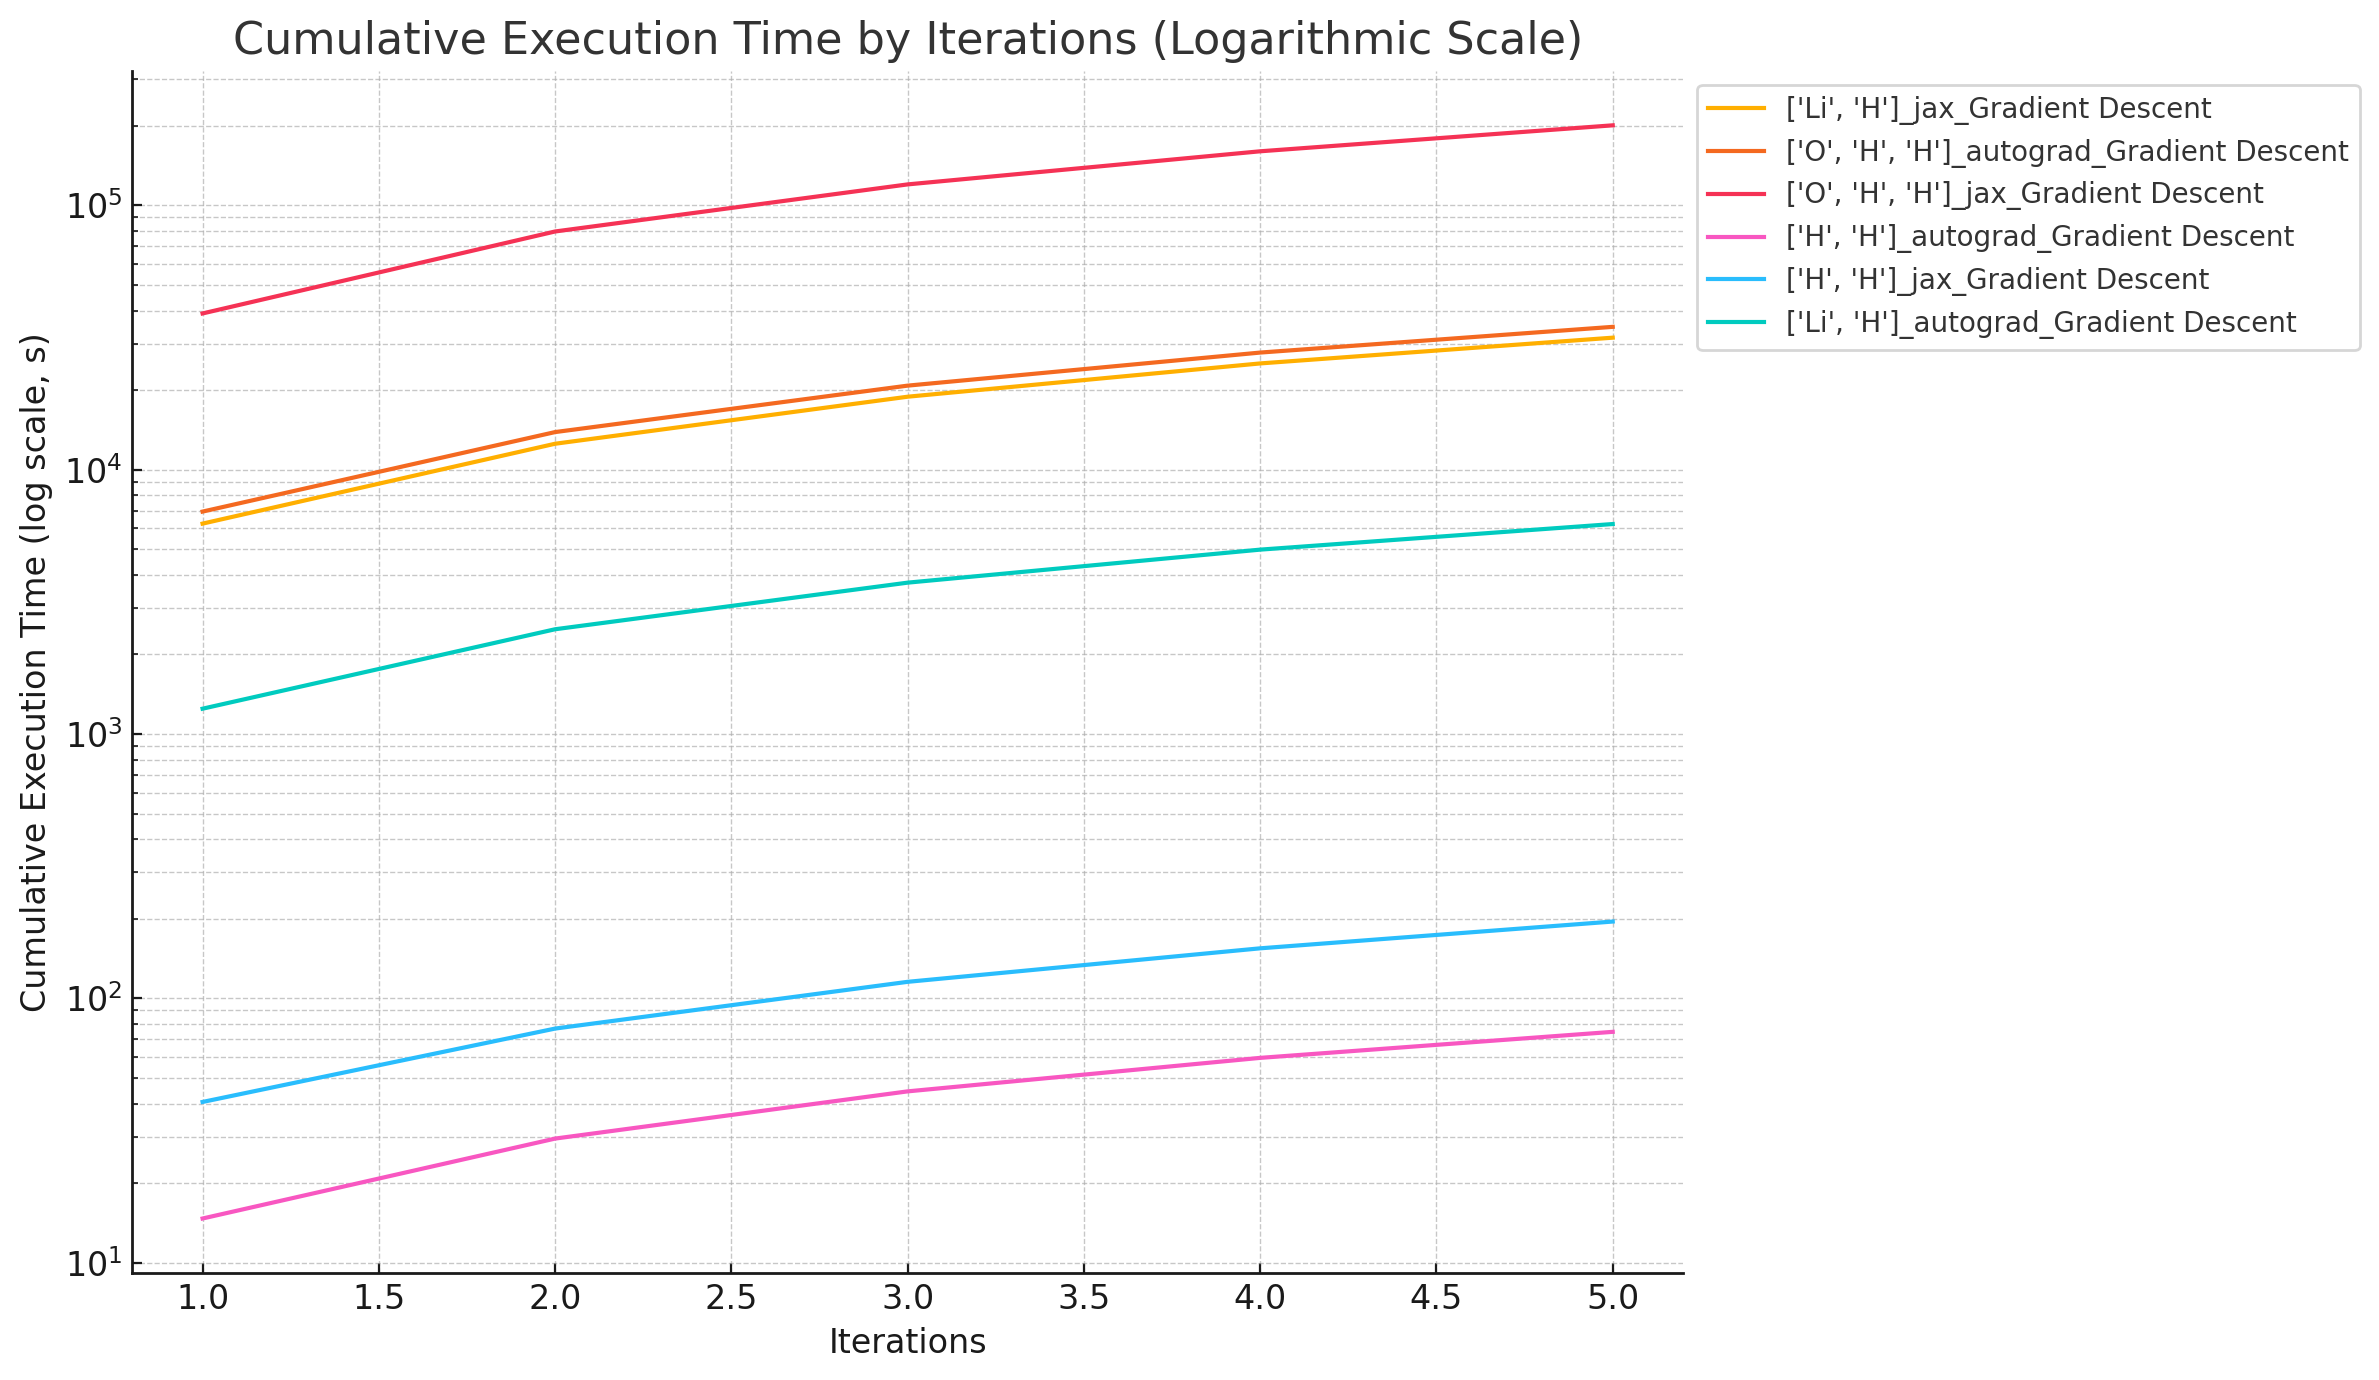
\includegraphics[width=0.8\textwidth]{img/time_iterations.png}
  \caption{Execution time of different molecules per iteration in the simulation.}
  \label{fig:time_iterations}
\end{figure}

\subsubsection{Comparative Performance Analysis}
To evaluate the performance of both interfaces in more detail, a table was created showing the percentage increase in execution time of \textit{JAX} compared to \textit{autograd}, as seen in Table~\ref{tab:jax_vs_auto}.

\begin{table}[H]
  \centering
  \scriptsize
  \resizebox{\textwidth}{!}{%
  \begin{tabular}{lcccc}
  \toprule
  \textbf{Metric} & 
  \textbf{LiH} & 
  \textbf{H\textsubscript{2}} & 
  \textbf{H\textsubscript{2}O} & 
  \textbf{Mean} \\
  \midrule
  \textbf{Total Time} & 80.28\% & 82.72\% & 61.75\% & 74.92\% \\
  \textbf{build\_hamiltonian} & 3.97\% & 8.49\% & 7.42\% & 6.63\% \\
  \textbf{compute\_operator\_gradients} & 91.24\% & 88.96\% & 94.70\% & 91.63\% \\
  \textbf{update\_parameters\_and\_coordinates} & 66.80\% & 74.62\% & 59.70\% & 67.04\% \\
  \bottomrule
  \end{tabular}%
  }
  \caption{Comparison of execution times between JAX and autograd interfaces for different molecules.}
  \label{tab:jax_vs_auto}
\end{table}

On average, it was observed that the \textit{JAX} interface exhibits a 74.92\% higher total execution time than the \textit{autograd} interface. Additionally, it is interesting to note that as the complexity of the molecule increases (with a greater number of atoms), the penalty percentage of \textit{JAX} tends to decrease. This behavior suggests that, in larger-scale problems, GPU acceleration could become more competitive, although it does not manage to outperform \textit{autograd} in this implementation.

\subsection{Computation Time per Function}
For a higher level of detail, the computation time was also measured for each part of the code where the interface change is introduced. Figure~\ref{fig:time_functions} shows the accumulated execution times in the main stages of the algorithm.

\begin{figure}[H]
  \centering
  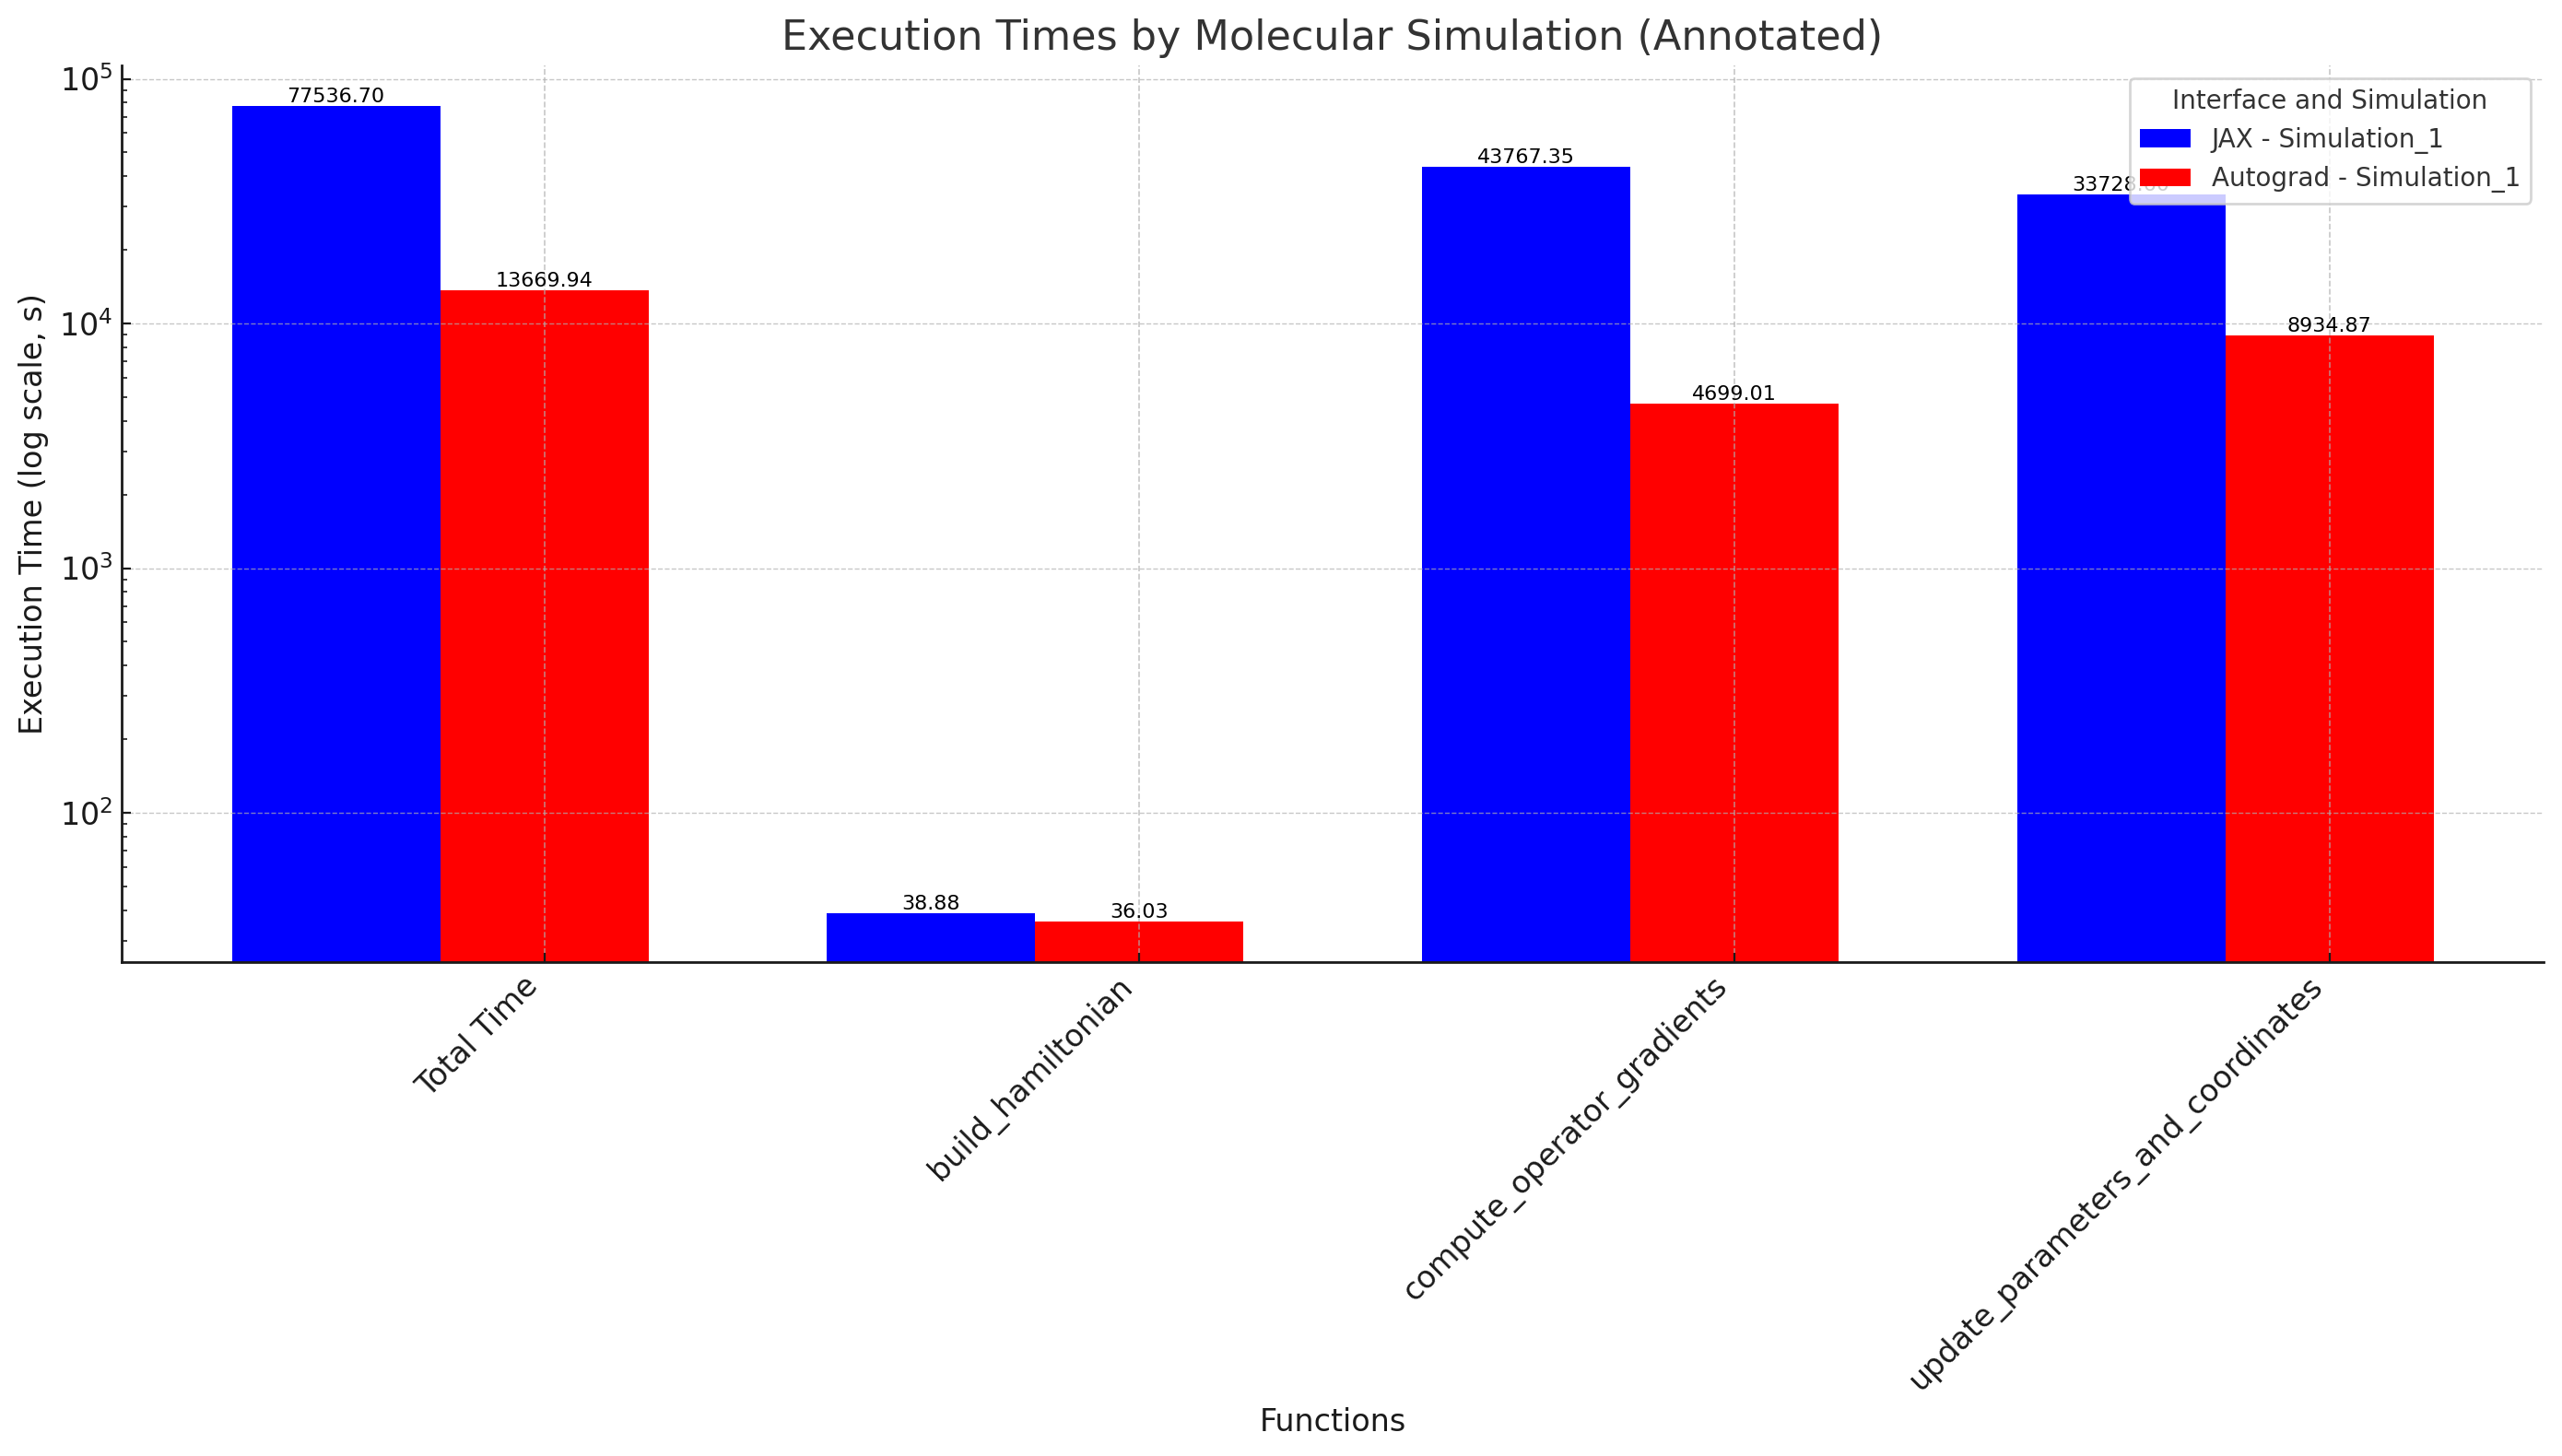
\includegraphics[width=0.8\textwidth]{img/time_functions.png}
  \caption{Execution time in different parts of the code.}
  \label{fig:time_functions}
\end{figure}

The same pattern is maintained in all functions: the \textit{JAX} interface records higher execution times than \textit{autograd}. In particular, the gradient computation part \texttt{compute\_operator\_gradients} increases its execution time by 91.68\% when using \textit{JAX}. This difference is largely attributed to the overhead caused by data transfer between the CPU and GPU, especially given that \textit{PennyLane} does not fully support Hamiltonian generation on the GPU.

On the other hand, the function \texttt{update\_parameters\_and\_coordinates}, responsible for performing the molecular geometry and parameter optimization step, also shows a 67.04\% increase when using \textit{JAX}. Nevertheless, it is worth highlighting that as the problem grows in complexity, the \textit{JAX} interface gains some relative efficiency in gradient calculation; however, the time saved through GPU acceleration is offset by the continuous data transfer between CPU and GPU throughout the iterations.

\subsection{Conclusions}
Based on the obtained results, the \textit{autograd} interface demonstrated superior performance in terms of speed for our implementation of the quantum molecular simulator. Although the GPU is usually advantageous in larger-scale problems, the data transfer overhead and the lack of full support for Hamiltonian generation within the GPU reduced the efficiency of \textit{JAX}. For this reason, we ultimately chose to use the \textit{autograd} interface for the final implementation of the quantum molecular simulator.

\section{Ansatz Comparison}
One of the most significant modifications affecting our code and its functionality has been the choice of the Ansatz. Our proposal has been to implement UCCSD, an Ansatz typically used for this type of simulation, as it enhances the simulation performance by achieving higher efficiency. The efficacy of this type of Ansatz has already been demonstrated, showing how it can improve simulation performance by producing more optimal quantum circuits without the need to create a specific Ansatz for the molecule being simulated. Indeed, for each optimizer configuration and for each different molecule simulation, there exists an optimal quantum circuit that achieves the best performance. However, since our objective is to develop a program that can simulate various molecules with maximum performance, we observe that the best option is UCCSD. To illustrate how our simulation performance is improved, we have generated Ansätze with different levels of depth and compared their performance with that of a UCCSD Ansatz. We have simulated various configurations of classical Ansätze, and in all cases, the UCCSD Ansatz has achieved better performance. More complex and molecule-specific Ansätze could be tested, but it is unlikely that another type of Ansatz would outperform UCCSD in terms of performance improvement.

Below is a simulation with different Ansatz depths and varying numbers of iterations obtained directly from the simulation.

\begin{figure}[H]
  \centering
  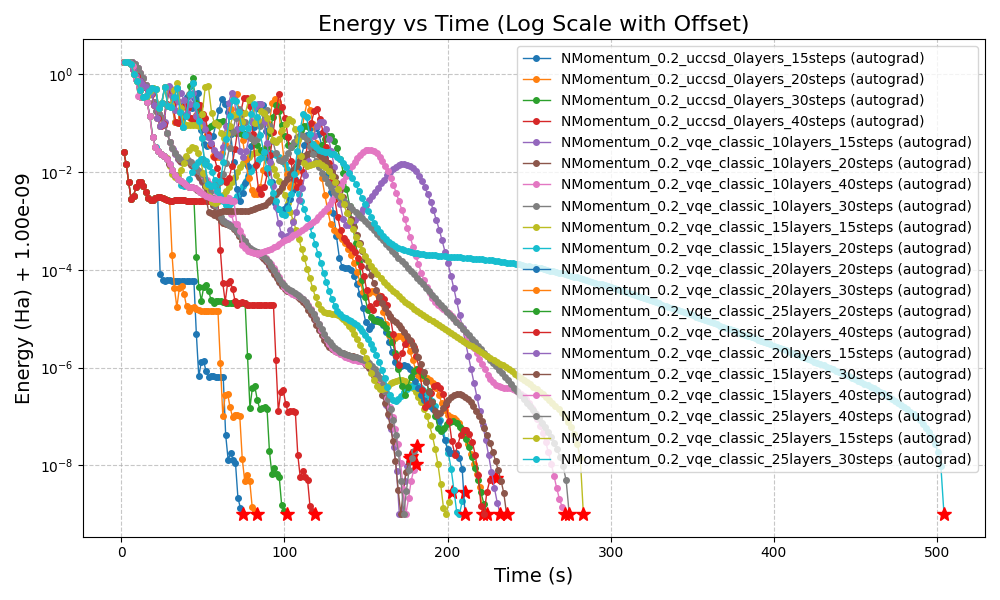
\includegraphics[width=0.8\textwidth]{data/Anzatz/results_ansatz_lyers_dif_iterations/energy_vs_time_log_offset.png}
  \caption{Energy vs. Time for different Ansätze and iterations.}
  \label{fig:ansatz_layers_iterations}
\end{figure}

It is observed that the UCCSD Ansatz achieves the best performance in all simulations, regardless of the number of optimizations performed for each iteration. For greater clarity of the results, a simulation was conducted with only a single number of optimizations per iteration, and the performance of the different Ansätze was compared, providing a clearer view of how UCCSD achieves the optimal performance.

\begin{figure}[H]
  \centering
  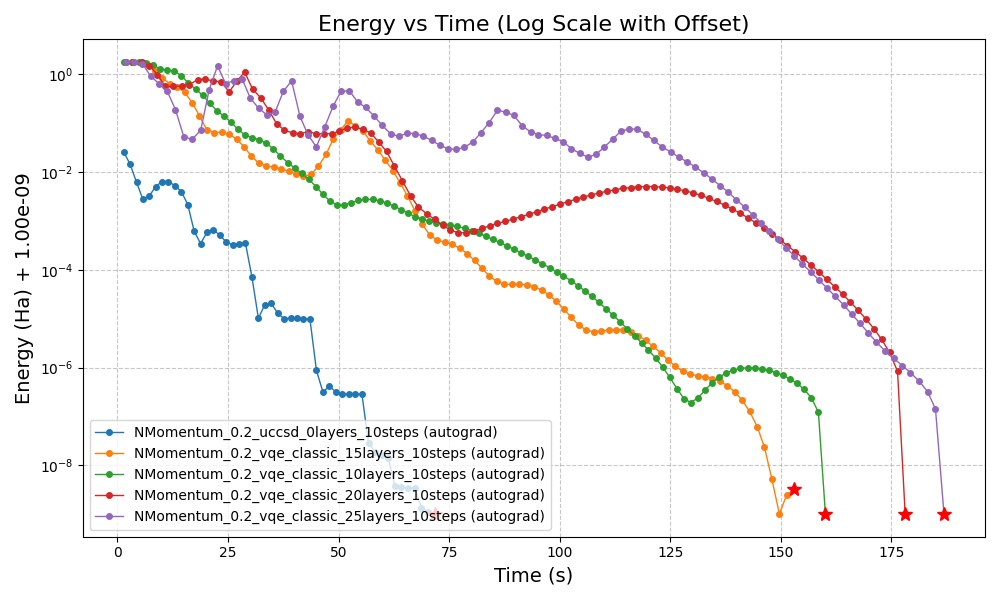
\includegraphics[width=0.8\textwidth]{data/Anzatz/results_ansatz_lyers/energy_vs_time_log_offset.png}
  \caption{Energy vs. Time for different Ansätze.}
  \label{fig:ansatz_layers}
\end{figure}

Finally, to corroborate that the UCCSD Ansatz achieves the best performance, a simulation was conducted with a different molecule, and the performance of the various Ansätze was compared. In the following image, it can be seen that the UCCSD Ansatz achieves highest efficiency in all simulations.

\section{Optimizer}

Once the Ansatz was selected, the next step was to test the functionality of our project, and thus see how it could help us improve the performance of our simulations. For this purpose, a series of tests were carried out using the capabilities previously designed for performance improvement. The tests were performed with a single Ansatz, UCCSD, and for the following molecules: H2, LiH, and H2O.

The steps followed for the realization of the tests were as follows:
\subsection{Optimizer Selection}
The first step was to determine the optimizer for the different molecules. To achieve this, we developed a procedure that allowed executing the same molecules with various optimizers, each covering a range of \emph{step size} values. This approach enabled the comparison of the different optimizers to be as fair as possible.

In the first phase, which executed 42 processes in parallel, observing which \emph{step size} offered the best performance for each optimizer and molecule. Subsequently, the simulation was repeated using only those optimal \emph{step sizes}, thereby achieving greater accuracy in the optimal \emph{step size} value for each optimizer, which will be discussed in the next section. The results of this second simulation are presented below.


\begin{figure}[H]
  \centering
  % First image
  \begin{subfigure}{0.45\textwidth}
    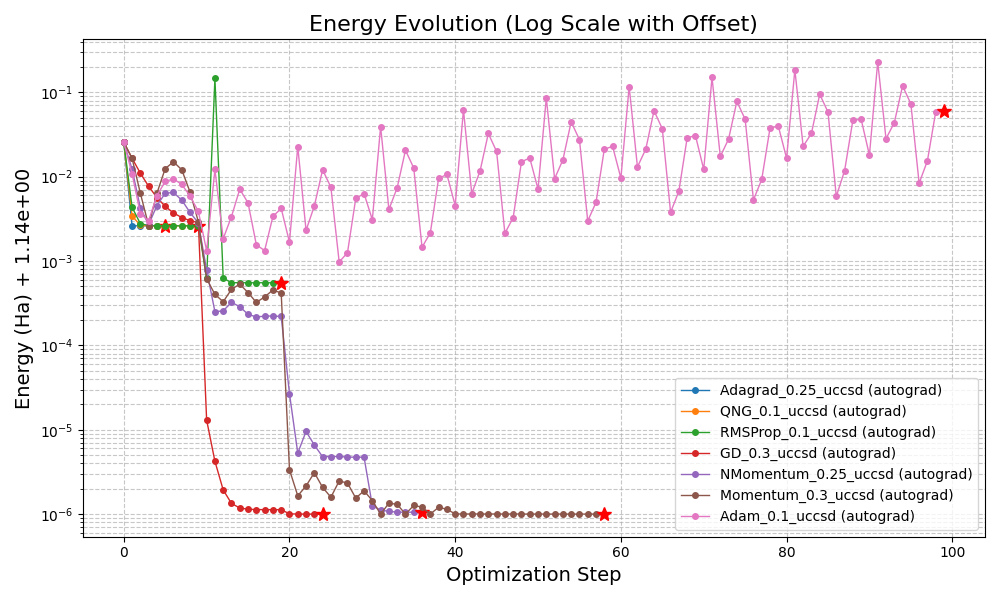
\includegraphics[width=\textwidth]{data/Optimizadores/final_results_H2/energy_evolution_log_offset.png}
    \caption{H2 simulation.}
    \label{fig:subimage1}
  \end{subfigure}
  % Second image
  \begin{subfigure}{0.45\textwidth}
    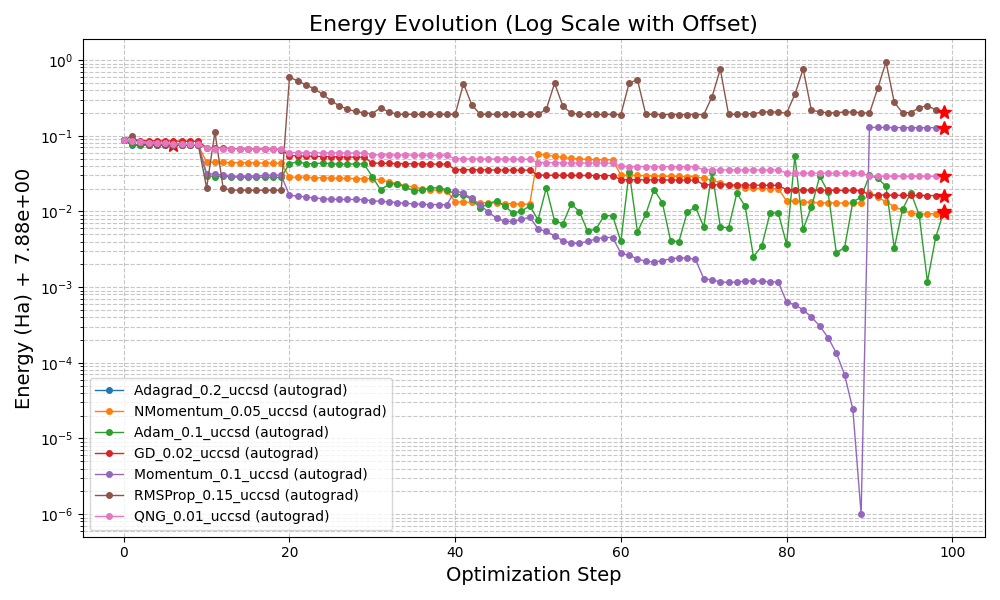
\includegraphics[width=\textwidth]{data/Optimizadores/final_results_LiH/energy_evolution_log_offset.png}
    \caption{LiH simulation.}
    \label{fig:subimage2}
  \end{subfigure}
  % Third image
  \begin{subfigure}{0.45\textwidth}
    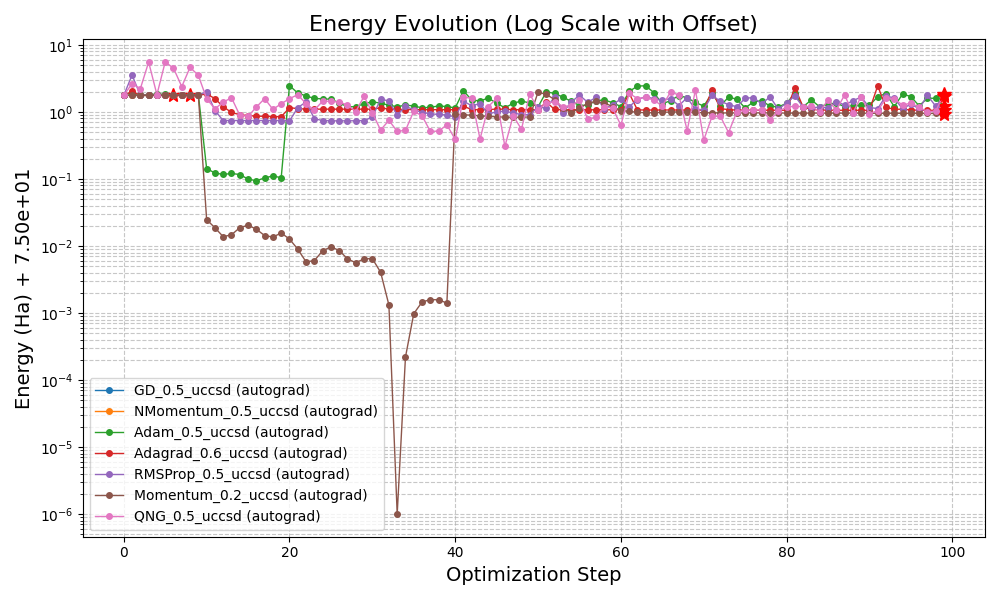
\includegraphics[width=\textwidth]{data/Optimizadores/final_results_H20/energy_evolution_log_offset.png}
    \caption{H2O simulation.}
    \label{fig:subimage3}
  \end{subfigure}
  \caption{Optimal \emph{step size} selection for each optimizer and molecule.}
  \label{fig:three_images}
\end{figure}

To delve deeper into the performance of the different optimizers, the following tables present the final energy, total optimization time, and the number of iterations required to converge for each molecule.

\begin{table}[H]
  \centering
  \caption{Final energy and optimization time for \(\mathrm{H_2}\), \(\mathrm{LiH}\), and \(\mathrm{H_2O}\) using various optimizers.}
  \begin{scriptsize}
  \begin{tabular}{lcccc}
  \toprule
  \textbf{Molecule} & \textbf{Optimizer} & \textbf{Final Energy (Ha)} & \textbf{Total Time (s)} & \textbf{Iterations} \\
  \midrule
  \multirow{7}{*}{\(\mathrm{H_2}\)} 
  & Adam (0.1)       & -1.07655292  & 173.30  & 10 \\
  & Adagrad (0.25)   & -1.13469066  & 10.19   & 1 \\
  & NMomentum (0.25) & -1.13730600  & 62.84   & 4 \\
  & Momentum (0.3)   & \(\mathbf{-1.13730605}\) & 100.43 & 6 \\
  & RMSProp (0.1)    & -1.13675411  & 33.14   & 2 \\
  & GD (0.3)         & \(\mathbf{-1.13730605}\) & 41.77  & 3 \\
  & QNG (0.1)        & -1.13469066  & 18.40   & 1 \\
  \midrule
  \multirow{7}{*}{\(\mathrm{LiH}\)} 
  & Adam (0.1)       & -7.87024707  & 13444.57 & 10 \\
  & Adagrad (0.2)    & -7.80548501  & 977.86   & 1 \\
  & NMomentum (0.05) & \(\mathbf{-7.87085783}\) & 13442.59 & 10 \\
  & Momentum (0.1)   & -7.75267240  & 13566.98 & 10 \\
  & RMSProp (0.15)   & -7.67650000  & 13671.22 & 10 \\
  & GD (0.02)        & -7.86422129  & 13449.49 & 10 \\
  & QNG (0.01)       & -7.85120449  & 13776.00 & 10 \\
  \midrule
  \multirow{7}{*}{\(\mathrm{H_2O}\)} 
  & Adam (0.5)       & -73.75990609 & 28454.49 & 10 \\
  & Adagrad (0.6)    & -73.93046296 & 28891.08 & 10 \\
  & NMomentum (0.5)  & -73.22152796 & 7497.83  & 1 \\
  & Momentum (0.2)   & \(\mathbf{-74.03997489}\) & 68420.47 & 10 \\
  & RMSProp (0.5)    & -73.28585876 & 65470.02 & 10 \\
  & GD (0.5)         & -73.22152796 & \(\mathbf{6486.79}\) & 1 \\
  & QNG (0.5)        & -73.13971041 & 70716.22 & 10 \\
  \bottomrule
  \end{tabular}
  \end{scriptsize}
\end{table}
  

In the evolution of the 3 iterations, we observed that the \textit{Momentum} optimizer was the one that offered the best performance in all the molecules. In the case of LiH, it is observed that it converges best until it reaches a geometric optimization, at which point it fails to converge. This is because the \emph{step size} is not yet fully optimized. Even so, we conclude that for the three simulations, the \textit{Momentum} optimizer is the one that offers the best performance.

An optimizer that also offers good performance is \textit{Adagrad}. Although it does not converge as effectively as \textit{Momentum}, it provides great speed in the simulations.

\newpage
\subsection{Step Size Selection}
To determine the most suitable \textit{step size} range, we started with the optimal value identified during optimizer selection. Subsequently, additional simulations were designed with values close to the initial optimum to refine this selection. 

This section presents the evolution of energy as a function of iterations, considering different \textit{step size} values for each molecule.

\begin{figure}[H]
  \centering
  % First image
  \begin{subfigure}{0.45\textwidth}
    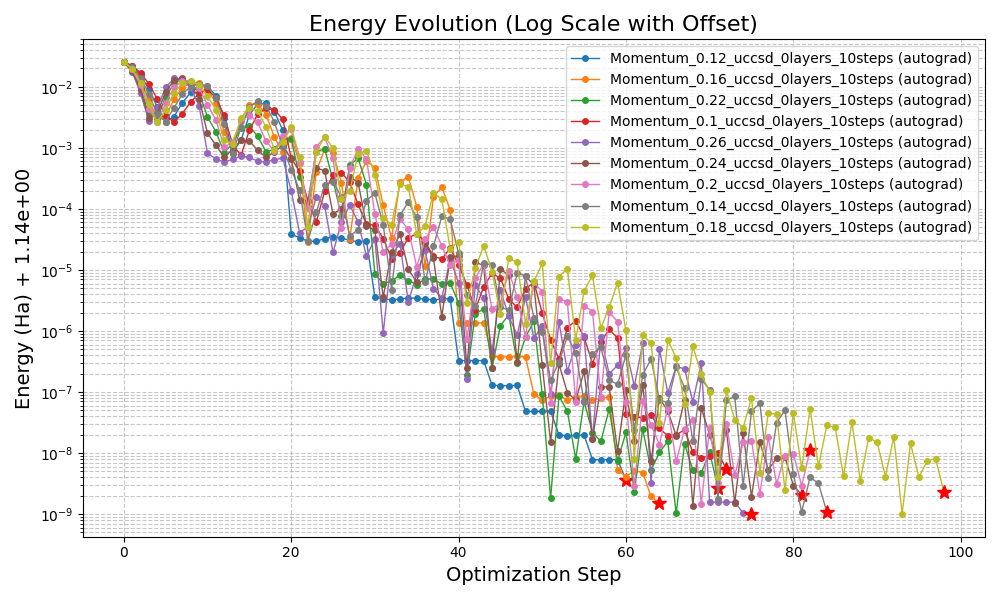
\includegraphics[width=\textwidth]{data/Stepsize/results_H2/energy_evolution_log_offset.png}
    \caption{H$_2$ simulation.}
    \label{fig:step_size_h2}
  \end{subfigure}
  % Second image
  \begin{subfigure}{0.45\textwidth}
    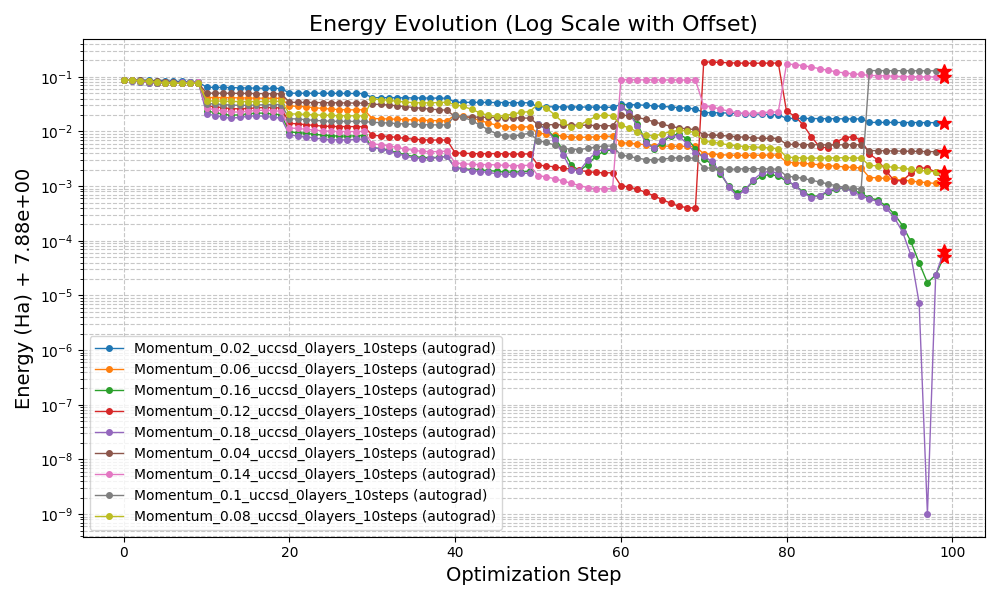
\includegraphics[width=\textwidth]{data/Stepsize/results_LiH/energy_evolution_log_offset.png}
    \caption{LiH simulation.}
    \label{fig:step_size_lih}
  \end{subfigure}
  % Third image
  \begin{subfigure}{0.45\textwidth}
    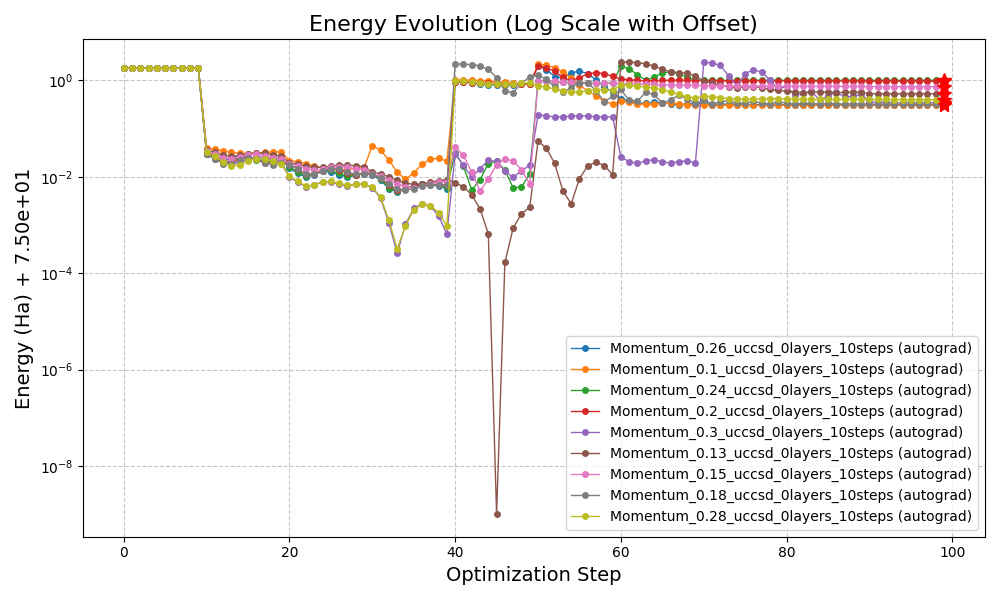
\includegraphics[width=\textwidth]{data/Stepsize/results_H2O/energy_evolution_log_offset.png}
    \caption{H$_2$O simulation.}
    \label{fig:step_size_h2o}
  \end{subfigure}
  \caption{Energy evolution as a function of \textit{step size} for different molecules.}
  \label{fig:step_size_results}
\end{figure}
Observing the graphs, we were able to see that for the molecules \(\mathrm{H_2}\) and \(\mathrm{LiH}\), the optimal \emph{step size} was clear, being 0.12 and 0.16 respectively. However, it was observed that for the molecule \(\mathrm{H_2O}\), the optimal \emph{step size} was not as clear, as there were several values that offered good performance.

For this reason, we created a table again to better observe the results. Note that in this case, each row corresponds to a \textit{step size}, keeping the same optimizer (  case, \textbf{Momentum}).

\begin{table}[H]
  \centering
  \caption{Final energy and optimization time for \(\mathrm{H_2}\), \(\mathrm{LiH}\), and \(\mathrm{H_2O}\) varying the \textit{step size} (optimizer: Momentum).}
  \begin{scriptsize}
  \begin{tabular}{lcccc}
  \toprule
  \textbf{Molecule} & \textbf{Step Size} & \textbf{Final Energy (Ha)} & \textbf{Total Time (s)} & \textbf{Iterations} \\
  \midrule
  \multirow{9}{*}{\(\mathrm{LiH}\)} 
  & 0.02 & -7.86678430 & \(\mathbf{13915.43}\) & 10 \\
  & 0.04 & -7.87699744 & 14001.06 & 10 \\
  & 0.06 & -7.88014045 & 13916.11 & 10 \\
  & 0.08 & -7.87944832 & 14144.26 & 10 \\
  & 0.10 & -7.75267240 & 14098.79 & 10 \\
  & 0.12 & -7.87992395 & 13937.66 & 10 \\
  & 0.14 & -7.78203292 & 14063.16 & 10 \\
  & 0.16 & \(\mathbf{-7.88118152}\) & 13931.81 & 10 \\
  & 0.18 & -7.88116774 & 13998.38 & 10 \\
  \midrule
  \multirow{9}{*}{\(\mathrm{H_2}\)} 
  & 0.10 & \(\mathbf{-1.13730605}\) & 113.23 & 10 \\
  & 0.12 & \(\mathbf{-1.13730605}\) & \(\mathbf{92.55}\) & 10 \\
  & 0.14 & \(\mathbf{-1.13730605}\) & 131.52 & 10 \\
  & 0.16 & \(\mathbf{-1.13730605}\) & 101.46 & 10 \\
  & 0.18 & \(\mathbf{-1.13730605}\) & 149.96 & 10 \\
  & 0.20 & -1.13730604 & 128.31 & 10 \\
  & 0.22 & \(\mathbf{-1.13730605}\) & 111.54 & 10 \\
  & 0.24 & \(\mathbf{-1.13730605}\) & 123.74 & 10 \\
  & 0.26 & \(\mathbf{-1.13730605}\) & 115.02 & 10 \\
  \midrule
  \multirow{9}{*}{\(\mathrm{H_2O}\)} 
  & 0.10 & \(\mathbf{-74.68985518}\) & 48577.15 & 10 \\
  & 0.13 & -74.46832273 & 74175.94 & 10 \\
  & 0.15 & -74.25355192 & 74211.21 & 10 \\
  & 0.18 & -74.67526296 & 75127.97 & 10 \\
  & 0.20 & -74.03997489 & 73130.72 & 10 \\
  & 0.24 & -73.99558215 & 56465.58 & 10 \\
  & 0.26 & -74.68963596 & \(\mathbf{44970.94}\) & 10 \\
  & 0.28 & -74.59437540 & 75555.08 & 10 \\
  & 0.30 & -74.65314486 & 73575.44 & 10 \\
  \bottomrule
  \end{tabular}
\end{scriptsize}
\end{table}

Finally, thanks to the table, we were able to see that, for \(\mathrm{H_2O}\), the \textit{step size} 0.10 was the one that gave the most optimal energy value, being slightly superior to 0.26.

Thus, we conclude that the optimal \textit{step size} values for the \textit{Momentum} optimizer are those found between 0.1 and 0.2, specifically, 0.12 for \(\mathrm{LiH}\), 0.12 for \(\mathrm{H_2}\), and 0.10 for \(\mathrm{H_2O}\).

\subsection{Number of Subiterations}

Finally, the last step that we performed to improve the performance of the simulation was in the number of subiterations that the optimization performs. By this, we refer to the iterations that are performed to optimize the parameters of each geometric position that we are optimizing the molecule. Since this is the process where most computational cost is incurred, it is a crucial step to improve the performance of the simulation.

To be able to configure in the most effective way the number of subiterations, we have generated a series of simulations with different numbers of subiterations, and we have observed the evolution of the energy. The configuration of the optimizers has been with the optimal values that we have obtained from the previous tests, with the Momentum optimizer and the step size values optimal for each molecule. Finally, the results have been compared with the values obtained from the following database: \href{https://cccbdb.nist.gov/}{NIST Computational Chemistry Comparison and Benchmark DataBase}.

Below are the graphs obtained from the different simulations:

\begin{figure}[H]
  \centering
  % First image
  \begin{subfigure}{0.45\textwidth}
    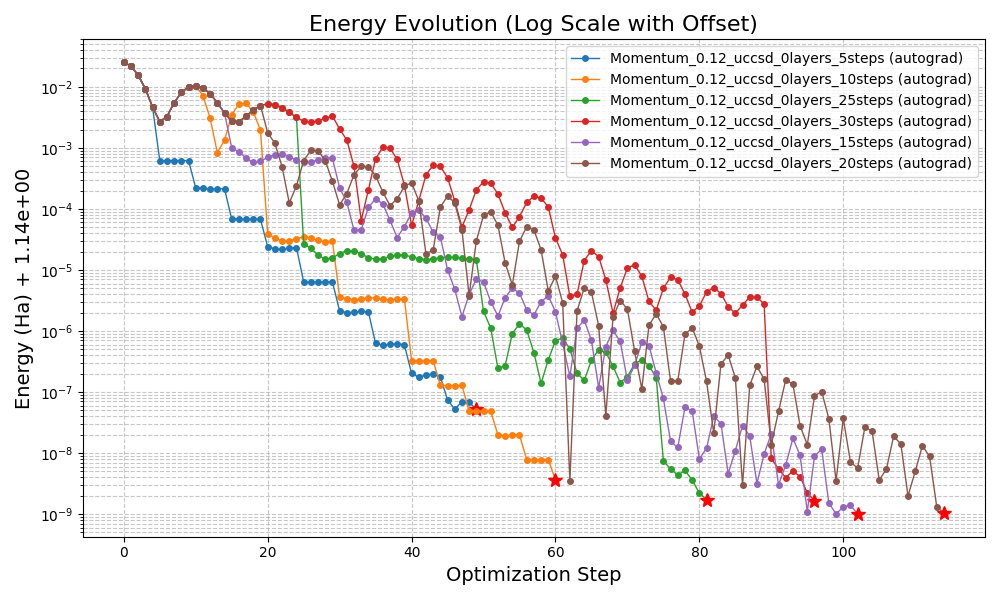
\includegraphics[width=\textwidth]{data/NumIterations/results_H2/energy_evolution_log_offset.png}
    \caption{H$_2$ simulation.}
    \label{fig:num_iterations_h2}
  \end{subfigure}
  % Second image
  \begin{subfigure}{0.45\textwidth}
    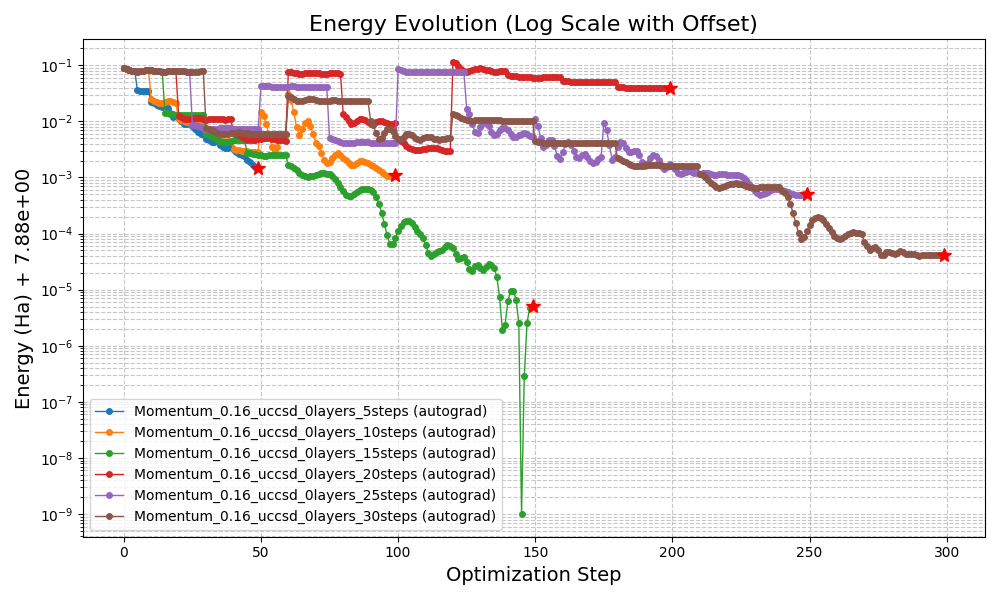
\includegraphics[width=\textwidth]{data/NumIterations/results_LiH/energy_evolution_log_offset.png}
    \caption{LiH simulation.}
    \label{fig:num_iterations_lih}
  \end{subfigure}
  % Third image
  \begin{subfigure}{0.45\textwidth}
    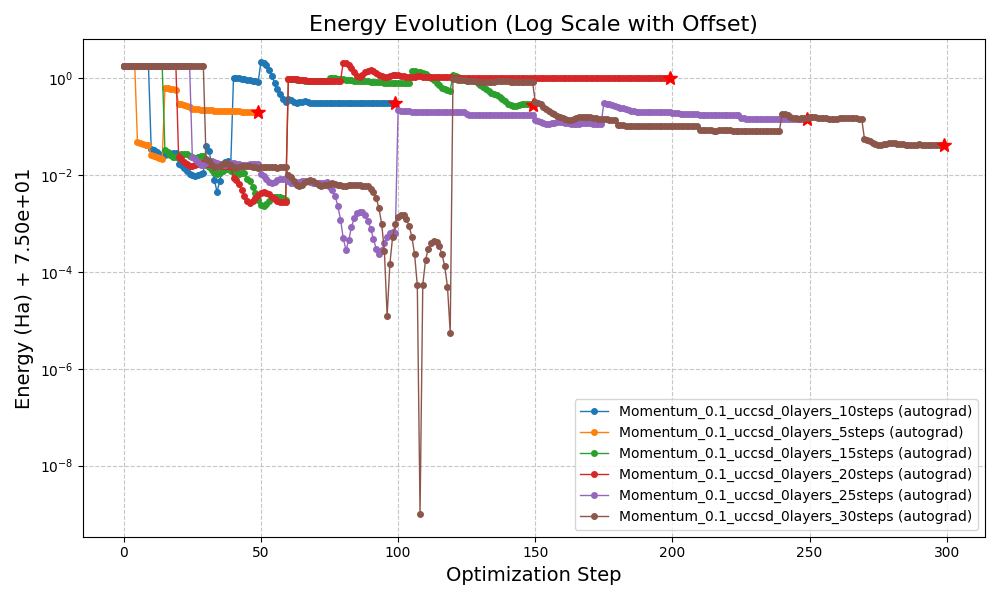
\includegraphics[width=\textwidth]{data/NumIterations/results_H2O/energy_evolution_log_offset.png}
    \caption{H$_2$O simulation.}
    \label{fig:num_iterations_h2o}
  \end{subfigure}
  \caption{Energy evolution as a function of \textit{number of iterations} for different molecules.}
  \label{fig:num_iterations_results}
\end{figure}

\subsubsection{Initial Results}

As in previous sections, to clarify the results, we have generated tables of the results that serve as tools for analyzing the outcomes in greater depth.

\begin{table}[H]
  \centering
  \caption{Final energy and optimization time for \(\mathrm{H_2}\), \(\mathrm{LiH}\), and \(\mathrm{H_2O}\) using Momentum optimizer with varying steps.}
  \begin{scriptsize}
  \begin{tabular}{lcccc}
  \toprule
  \textbf{Molecule} & \textbf{Steps} & \textbf{Final Energy (Ha)} & \textbf{Total Time (s)} & \textbf{Difference from FCI (Ha)} \\
  \midrule
  \multirow{6}{*}{\(\mathrm{H_2}\)} 
  & 5  & \(\mathbf{-1.13730605}\) & 101.86 & 0.00000005 \\
  & 10 & \(\mathbf{-1.13730605}\) & \(\mathbf{99.08}\) & 0.00000005 \\
  & 15 & \(\mathbf{-1.13730605}\) & 163.25 & 0.00000005 \\
  & 20 & \(\mathbf{-1.13730605}\) & 175.06 & 0.00000005 \\
  & 25 & \(\mathbf{-1.13730605}\) & 124.58 & 0.00000005 \\
  & 30 & \(\mathbf{-1.13730605}\) & 147.59 & 0.00000005 \\
  \midrule
  \multirow{6}{*}{\(\mathrm{LiH}\)} 
  & 5  & \(-7.88079149\) & \(\mathbf{8328.30}\) & 0.00174651 \\
  & 10 & \(-7.88118152\) & 13365.38 & \(\mathbf{0.00135648}\) \\
  & 15 & \(-7.88226478\) & 18384.78 & 0.00027322 \\
  & 20 & \(-7.84260017\) & 23309.87 & 0.03993783 \\
  & 25 & \(-7.88176386\) & 28433.90 & 0.00077414 \\
  & 30 & \(\mathbf{-7.88222895}\) & 33421.15 & \(\mathbf{0.00030905}\) \\
  \midrule
  \multirow{6}{*}{\(\mathrm{H_2O}\)} 
  & 5  & \(-74.79245495\) & \(\mathbf{50836.87}\) & \(0.22251505\) \\
  & 10 & \(-74.68985518\) & 45559.48 & \(0.32511482\) \\
  & 15 & \(-74.70554258\) & 77448.07 & \(0.30942742\) \\
  & 20 & \(-74.00851054\) & 113172.24 & \(1.00645946\) \\
  & 25 & \(-74.84425344\) & 136497.21 & \(0.17071656\) \\
  & 30 & \(\mathbf{-74.94705746}\) & 157949.56 & \(\mathbf{0.06791254}\) \\
  \bottomrule
  \end{tabular}
  \end{scriptsize}
\end{table}

  
We clearly observe that for the molecule \(\mathrm{H_2}\), the number of subiterations does not affect the final result. In this case, as it is such a basic molecule with few parameters, the simulation converges relatively easily for all configurations. Thus, we observe that the best option, due to its speed and accuracy, and yielding the best performance, is the configuration with 10 subiterations per geometric position, with an execution time of 99.08 seconds, being 2.72\% faster than the configuration with 5 subiterations.

In the case of \(\mathrm{LiH}\), the energy \(-7.88222895\,\mathrm{Ha}\) achieved in 30 steps shows the best accuracy compared to the reference value. However, as we are interested in a balance between performance and accuracy, by observing the execution times and results, we find that the optimal performances are achieved with a number of subiterations between 5 and 10 per geometric optimization cycle. Considering that the accuracy with 10 subiterations is 22.33\% higher but with a 37.68\% increase in computation time, we conclude that the process with highest efficiency is that with 5 subiterations.

For the molecule \(\mathrm{H_2O}\), we find the same result as for the molecule \(\mathrm{LiH}\), where the highest accuracy is obtained with 30 subiterations, but the best performance is achieved with 5 to 10 subiterations per cycle. Making the same comparison as before, we find that with 10.38\% less computation, we obtain 31.55\% less accuracy, so the optimal performance is achieved with 5 subiterations.

The results show that highest efficiency is found between 5 and 10 subiterations per geometric optimization cycle, achieving a balance between accuracy and computation time. This leads us to conclude that the best option is 10 subiterations for the molecule \(\mathrm{H_2}\), and 5 subiterations for the molecules \(\mathrm{LiH}\) and \(\mathrm{H_2O}\). For this reason, we have decided to analyze how these molecules evolve with this number of subiterations. The results obtained are presented below.

\subsubsection{Final phase}
To find a more precise value for the optimal number of subiterations, we conducted the same simulations as in the previous sections, but varying the number of subiterations in our simulations, setting them to values from 2 to 10. This allowed us to observe more clearly how the hybrid optimization technique implemented in our project affects the results.

\begin{figure}[H]
  \centering
  % First image
  \begin{subfigure}{0.45\textwidth}
    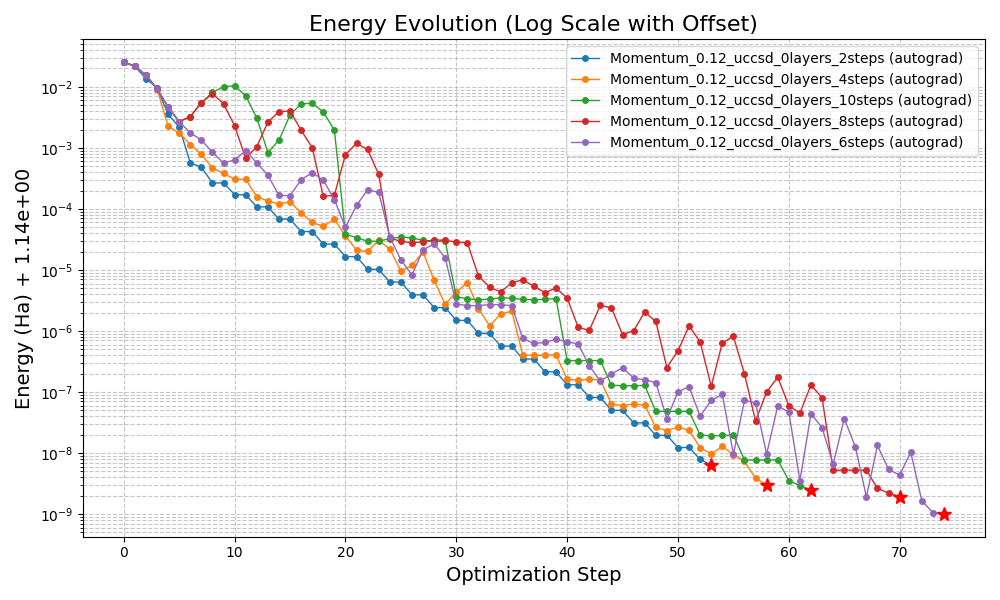
\includegraphics[width=\textwidth]{data/NumIterations/final_results_H2/energy_evolution_log_offset.png}
    \caption{H$_2$ simulation.}
    \label{fig:num_iterations_final_h2}
  \end{subfigure}
  % Second image
  \begin{subfigure}{0.45\textwidth}
    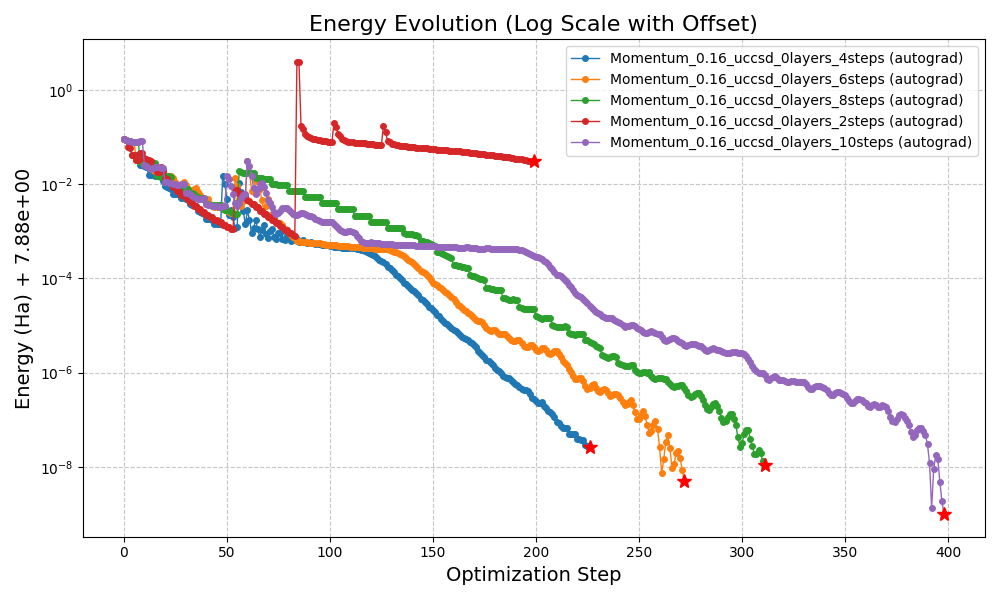
\includegraphics[width=\textwidth]{data/NumIterations/final_results_LiH/energy_evolution_log_offset.png}
    \caption{LiH simulation.}
    \label{fig:num_iterations_final_lih}
  \end{subfigure}
  % Third image
  \begin{subfigure}{0.45\textwidth}
    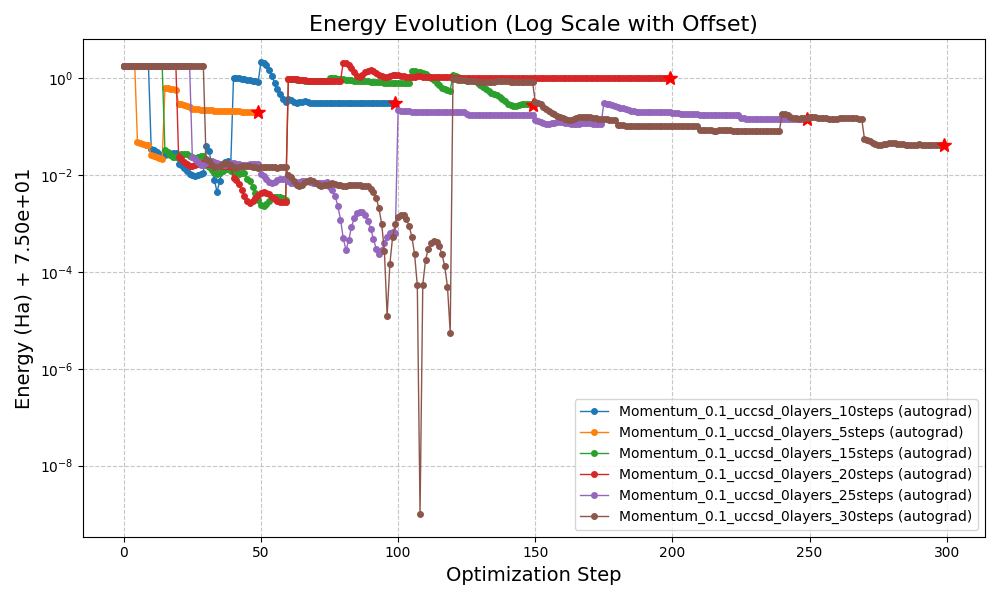
\includegraphics[width=\textwidth]{data/NumIterations/results_H2O/energy_evolution_log_offset.png}
    \caption{H$_2$O simulation.}
    \label{fig:num_iterations_final_h2o}
  \end{subfigure}
  \caption{Energy evolution as a function of \textit{number of iterations} for different molecules.}
  \label{fig:num_iterations_final_results}
\end{figure}
In the graphs obtained from this second simulation, the effect of hybrid optimization on convergence is clearly observed. The fewer the number of subiterations, the faster the convergence. However, this has a negative effect, as the optimization becomes more unstable and imprecise. We observe that in the molecule \(\mathrm{H_2}\), convergence is faster with 2 subiterations. In the case of \(\mathrm{LiH}\), the most effective simulation is with 4 subiterations. Additionally, it is observed that reducing to 2 subiterations causes the simulation to fail to converge due to the instability of the optimization. The data from both simulations are presented below.

\begin{table}[H]
  \centering
  \caption{Final energy and optimization time for \(\mathrm{H_2}\) and \(\mathrm{LiH}\).}
  \begin{scriptsize}
  \begin{tabular}{lcccc}
  \toprule
  \textbf{Molecule} & \textbf{Steps} & \textbf{Final Energy (Ha)} & \textbf{Total Time (s)} & \textbf{Difference from FCI (Ha)} \\
  \midrule
  \multirow{5}{*}{\(\mathrm{H_2}\)} 
    & 2  & \(-1.13730605\) & \textbf{95.57}  & \(0.00000005\) \\
    & 4  & \(-1.13730605\) & 96.65   & \(0.00000005\) \\
    & 6  & \(-1.13730605\) & 122.50  & \(0.00000005\) \\
    & 8  & \(-1.13730605\) & 111.27  & \(0.00000005\) \\
    & 10 & \(-1.13730605\) & 98.74   & \(0.00000005\) \\
  \midrule
  \multirow{5}{*}{\(\mathrm{LiH}\)} 
    & 2  & \(-7.85253665\) & 51461.91 & \(0.03000135\) \\
    & 4  & \(\mathbf{-7.88275270}\) & \(\mathbf{40118.76}\) & \(\mathbf{0.00021470}\) \\
    & 6  & \(-7.88275272\) & 40896.30 & \(0.00021472\) \\
    & 8  & \(-7.88275272\) & 43240.40 & \(0.00021472\) \\
    & 10 & \(-7.88275272\) & 43240.40 & \(0.00021472\) \\
  \bottomrule
  \end{tabular}
  \end{scriptsize}
\end{table}

\section{Limitations}
During the tests conducted, we identified various limitations that may have affected the results. The most significant limitation has been the lack of implementation of quantum error simulations. In all simulations, the negative effects of errors that can occur in real quantum computers have not been considered. For this reason, we cannot assert that these same results would be useful for a similar implementation on a real quantum computer.

Similarly, we did not have access to a quantum computer, which would have been extremely helpful in validating the proper functionality of our project. Even so, we have been able to verify that our project performs optimally and that the implementation of hybrid optimization is effective in improving the performance of the simulations.

Another limiting aspect has been the computational capacity of our computer. Since we do not have access to a quantum computer, simulations with a high number of molecules have been very costly in terms of computational time.


%%%% BUDGET %%%%
% Budget chapter. Please replace "budget.tex" entirely with your own content written in the desired language.
%\input{budget}


%%%% SUSTAINABILITY REPORT %%%%    <<<<<<<<<<<<<<<< NEW !!
% Sustainability chapter. Please replace "sustainability.tex" entirely with your own content written in the desired language.
%%%% PLEASE REPLACE ENTIRELY WITH YOUR OWN CONTENT %%%%

\ifcase\doclanguage\or
\chapter{Anàlisi de sostenibilitat i implicacions ètiques}
Des del curs 2023-24, la normativa de TFG de l'ETSETB demana la inclusió d'un informe de sostenibilitat a la memòria del treball. Aquesta anàlisi consisteix en una valoració dels impactes ambientals, socials i econòmics, i les possibles implicacions ètiques que ha comportat la realització del TFG. En el cas que el TFG plantegi un producte/servei/sistema/edifici/etc., que podria arribar a implementar-se, l’anàlisi també ha de realitzar-se sobre els impactes que tindria la proposta en la seva execució durant les diferents etapes del seu cicle de vida.

A la plataforma ATENEA trobareu un document separat amb les instruccions detallades de què ha de contenir i com cal confeccionar l'informe de sostenibilitat.

{\bigskip\bfseries {\large IMPORTANT:} Noteu que l'antic capítol de «Pressupost del projecte» ara queda integrat en l'anàlisi de sostenibilitat, concretament en les cel·les «Econòmic/Desenvolupament del TFG» i «Econòmic/Execució del projecte».}

\or
\chapter{Análisis de sostenibilidad e implicaciones éticas}
A partir del curso 2023-24, la normativa de TFG de la ETSETB solicita la inclusión de un informe de sostenibilidad en la memoria del trabajo. Este análisis consiste en una evaluación de los impactos ambientales, sociales y económicos, así como las posibles implicaciones éticas derivadas de la realización del TFG. En el caso de que el TFG plantee un producto/servicio/sistema/edificio, etc., que pudiera llegar a implementarse, el análisis también debe abordar los impactos que la propuesta tendría durante las diferentes etapas de su ciclo de vida.

En la plataforma ATENEA encontrarán un documento aparte con instrucciones detalladas sobre lo que debe contener y cómo elaborar el informe de sostenibilidad.

{\bigskip\bfseries {\large IMPORTANTE:} Tener en cuenta que el antiguo capítulo de «Presupuesto del proyecto» ahora se integra en el análisis de sostenibilidad, específicamente en las celdas «Económico/Desarrollo del TFG» y «Económico/Ejecución del proyecto».}

\else
\chapter{Sustainability Analysis and Ethical Implications}
Starting from the academic year 2023-24, the TFG regulations of ETSETB require the inclusion of a sustainability report in the project's documentation. This analysis involves an assessment of environmental, social, and economic impacts, as well as potential ethical implications resulting from the completion of the TFG. In the case where the TFG involves a product/service/system/building, etc., that could be implemented, the analysis should also address the impacts that the proposal would have during the various stages of its lifecycle.

Detailed instructions on what the sustainability report should contain and how to prepare it can be found on the ATENEA platform.

{\bigskip\bfseries {\large IMPORTANT:} Please note that the previous chapter on "Project Budget" is now integrated into the sustainability analysis, specifically in the cells "Economic Cell/Development of BT" and "Economic Cell/Project Execution".}

\fi


%%%% CONCLUSIONS AND FUTURE WORK %%%%
% Conclusions chapter. Please replace "conclusions.tex" entirely with your own content written in the desired language.
\chapter{Conclusions and Future Work}

\section{Conclusions}

In this project, we have successfully implemented a quantum simulator focused on simulating various molecular systems using the VQE algorithm. The results demonstrate the ability to optimize the processes for H$_2$, LiH, and H$_2$O, molecules of different sizes and complexities. Additionally, the efficacy of the UCCSD ansatz has been validated, achieving superior results compared to other ansätze. An unexpected outcome, which adds significant value to our project, was the demonstration that, for our implementation, the \textit{autograd} interface is more effective than JAX.

The contributions of this work to the field include the modular design of quantum simulation software, enabling extensibility and flexibility for future algorithms and optimization strategies. Furthermore, the introduction of an adaptive methodology for selecting different ansätze and optimizers has made the optimization process more efficient and faster.

With all this, the objectives of our project have been successfully achieved. These objectives include the development of an adaptive ansatz capable of selecting the operators with the greatest impact on the system, the integration of a hybrid optimization approach that adjusts both the ansatz parameters and nuclear positions, and endows our simulations with greater robustness and precision. Finally, the design of a modular architecture facilitates the inclusion of new types of ansätze and optimizers, enabling the comparison of different optimization strategies for future research.

\section{Future Directions}
In this project, the initial questions posed have been successfully addressed. However, after the completion of the project, new frontiers and research lines have emerged, offering exciting opportunities for future work.

During the development of the project, it became evident that the mixed optimization methodology could be improved by adding more complexity to the optimization process, thereby achieving greater efficiency in convergence. We realized that another viable option to enhance simulation convergence would be to implement an adaptive optimization system, which dynamically adjusts the number of optimizations of the ansatz parameters based on the simulation’s progress. This would result in greater efficiency in the simulation’s convergence. Additionally, it was observed that automating the configuration of optimizers would save considerable time during setup.

As a final future endeavor, to improve the simulator's consistency, it would be valuable to investigate its performance on NISQ systems. This would allow for an analysis of whether the implementation of a noise model affects the simulation's convergence, thus validating the robustness of the simulator in real-world quantum systems.

Another relevant research avenue would involve integrating error mitigation techniques, such as zero-noise extrapolation, to enhance the accuracy of simulations on noisy quantum devices. This would add greater realism to the simulations and make the simulator more practical for applications on current quantum hardware.

Finally, due to the modular nature of the simulator, it could be adapted to other fields beyond chemistry, such as material science and condensed matter physics. Exploring these areas would broaden its impact and leverage its flexibility for a wide range of scientific applications.


%%%% BIBLIOGRAPHY %%%%
\nocite{*}               % Forces all entries to be printed, even if not cited
% Bibliography intro
% Supress this macro (or modify its contents to suit your needs).
\defbibnote{bib-intro}{%
\ifcase\doclanguage\or
  El sistema \textit{biblatex} simplifica la gestió de la bibliografia en treballs científics, proporcionant automatització i personalització en el format de les citacions. Això permet a l'autor del document enfocar-se en el contingut sense haver de preocupar-se per l'estil de les referències, estalviant temps i reduint errors.
  
  La base de dades de referències bibliogràfiques és al fitxer «TFG.bib» i és allà on heu d'afegir les vostres referències. Consulteu el manual del \texttt{biblatex}, secció «Database Guide», per conèixer els tipus de referències i camps disponibles.
  
  Podeu modificar (o suprimir) aquesta nota editant la macro \texttt{\textbackslash defbibnote} al fitxer «TFG.tex».
  \par\hfil\rule[3pt]{.5\textwidth}{0.4pt}\hfil\par\or
  El sistema \textit{biblatex} simplifica la gestión de la bibliografía en trabajos científicos, proporcionando automatización y personalización en el formato de las citas. Esto permite al autor del documento enfocarse en el contenido sin tener que preocuparse por el estilo de las referencias, ahorrando tiempo y reduciendo errores.
  
  La base de datos de referencias bibliográficas está en el archivo «TFG.bib» y es allí donde se deben añadir vuestras referencias. Consultar el manual de \texttt{biblatex}, sección «Database Guide», para conocer los tipos de referencias y campos disponibles.
  
  Podéis modificar (o suprimir) esta nota editando la macro \texttt{\textbackslash defbibnote} en el archivo «TFG.tex».
  \par\hfil\rule[3pt]{.5\textwidth}{0.4pt}\hfil\par\else
  The \textit{biblatex} system simplifies the management of the bibliography in scientific works, providing automation and customization in the format of citations. This allows the document's author to focus on the content without having to worry about the style of the references, saving time and reducing errors.
  
  The bibliographic references database is in the file “TFG.bib”, and this is where you should add your references. Consult the \texttt{biblatex} manual, section “Database Guide”, to learn about the available types of references and fields.
  
  You can modify (or delete) this note by editing the \texttt{\textbackslash defbibnote} macro in the file “TFG.tex”.
  \par\hfil\rule[3pt]{.5\textwidth}{0.4pt}\hfil\par\fi%
}
\printbibliography[heading=bibintoc,prenote={bib-intro}]


%%%% ANNEXES %%%%
% All chapters AFTER the \appendix command wil be considered appendices and numbered by letter
\appendix
\chapter{Logic Gates}
\label{appendices:LogicGates}
\section{Simple Logic Gates}
Below are detailed the simple logic gates essential for constructing more complex quantum algorithms:

\paragraph{X Gate (Pauli-X)}

The \textbf{Pauli-X} gate is the quantum analog of the classical NOT gate. It performs a bit flip on the qubit, transforming the state $\ket{x}$ into $\ket{\neg x}$.

\vspace{0.5em}
\begin{minipage}{\textwidth}
    \begin{minipage}[t]{0.45\textwidth}
        \centering
        \textbf{Representative Matrix}\\[0.5em]
        \[
        X = 
        \begin{pmatrix}
        0 & 1 \\
        1 & 0 \\
        \end{pmatrix}
        \]
    \end{minipage}
    \hfill
    \begin{minipage}[t]{0.45\textwidth}
        \centering
        \textbf{Effect on Basis States}\\[0.5em]
        \begin{itemize}
            \item $X\ket{0} = \ket{1}$
            \item $X\ket{1} = \ket{0}$
        \end{itemize}
    \end{minipage}
\end{minipage}

\paragraph{Y Gate (Pauli-Y)}

The \textbf{Pauli-Y} gate performs a rotation of $\pi$ around the $y$-axis. It transforms the state $\ket{x}$ into $i(-1)^x\ket{\neg x}$.

\vspace{0.5em}

\begin{minipage}{\textwidth}
    \begin{minipage}[t]{0.45\textwidth}
        \centering
        \textbf{Representative Matrix}\\[0.5em]
        \[
        Y = 
        \begin{pmatrix}
        0 & -i \\
        i & 0 \\
        \end{pmatrix}
        \]
    \end{minipage}
    \hfill
    \begin{minipage}[t]{0.45\textwidth}
        \centering
        \textbf{Effect on Basis States}\\[0.5em]
        \begin{itemize}
            \item $Y\ket{0} = i\ket{1}$
            \item $Y\ket{1} = -i\ket{0}$
        \end{itemize}
    \end{minipage}
\end{minipage}

\paragraph{Z Gate (Pauli-Z)}

The \textbf{Pauli-Z} gate is known as the phase inversion gate. It transforms the state $\ket{x}$ into $(-1)^x\ket{x}$.

\vspace{0.5em}
\begin{minipage}{\textwidth}
    \begin{minipage}[t]{0.45\textwidth}
        \centering
        \textbf{Representative Matrix}\\[0.5em]
        \[
        Z = 
        \begin{pmatrix}
        1 & 0 \\
        0 & -1 \\
        \end{pmatrix}
        \]
    \end{minipage}
    \hfill
    \begin{minipage}[t]{0.45\textwidth}
        \centering
        \textbf{Effect on Basis States}\\[0.5em]
        \begin{itemize}
            \item $Z\ket{0} = \ket{0}$
            \item $Z\ket{1} = -\ket{1}$
        \end{itemize}
    \end{minipage}
\end{minipage}


\paragraph{Hadamard Gate (H)}

The \textbf{Hadamard} gate creates an equal superposition of the computational basis states. It transforms the state $\ket{x}$ into $\dfrac{1}{\sqrt{2}} (\ket{0} + (-1)^x \ket{1})$.

\vspace{0.5em}
\begin{minipage}{\textwidth}
    \begin{minipage}[t]{0.45\textwidth}
        \centering
        \textbf{Representative Matrix}\\[0.5em]
        \[
        H = \dfrac{1}{\sqrt{2}}
        \begin{pmatrix}
        1 & 1 \\
        1 & -1 \\
        \end{pmatrix}
        \]
    \end{minipage}
    \hfill
    \begin{minipage}[t]{0.45\textwidth}
        \centering
        \textbf{Effect on Basis States}\\[0.5em]
        \begin{itemize}
            \item $H\ket{0} = \dfrac{1}{\sqrt{2}} (\ket{0} + \ket{1}) = \ket{+}$
            \item $H\ket{1} = \dfrac{1}{\sqrt{2}} (\ket{0} - \ket{1}) = \ket{-}$
        \end{itemize}
    \end{minipage}
\end{minipage}

\section{Multi-Qubit Logic Gates}

\paragraph{Controlled-NOT Gate (CNOT)}

The \textbf{CNOT} or \textbf{Controlled-X} gate is a two-qubit gate that flips the second qubit (target) if and only if the first qubit (control) is in the state $\ket{1}$. It transforms the state $\ket{x, y}$ into $\ket{x, x \oplus y}$, where $\oplus$ denotes the XOR operation.

\vspace{0.5em}
\begin{minipage}{\textwidth}
    \begin{minipage}[t]{0.45\textwidth}
        \centering
        \textbf{Representative Matrix}\\[0.5em]
        \[
        \text{CNOT} = 
        \begin{pmatrix}
        1 & 0 & 0 & 0 \\
        0 & 1 & 0 & 0 \\
        0 & 0 & 0 & 1 \\
        0 & 0 & 1 & 0 \\
        \end{pmatrix}
        \]
    \end{minipage}
    \hfill
    \begin{minipage}[t]{0.45\textwidth}
        \centering
        \textbf{Effect on Basis States}\\[0.5em]
        \begin{itemize}
            \item $\text{CNOT}\ket{00} = \ket{00}$
            \item $\text{CNOT}\ket{01} = \ket{01}$
            \item $\text{CNOT}\ket{10} = \ket{11}$
            \item $\text{CNOT}\ket{11} = \ket{10}$
        \end{itemize}
    \end{minipage}
\end{minipage}

\paragraph{Single Excitation Gate (\textit{SingleExcitation})}

This gate performs a rotation in the two-dimensional subspace $\{\ket{01}, \ket{10}\}$. It transforms the state $\ket{10}$ into $\cos\left( \dfrac{\phi}{2} \right) \ket{10} - \sin\left( \dfrac{\phi}{2} \right) \ket{01}$.

\vspace{0.5em}
\begin{minipage}{\textwidth}
    \begin{minipage}[t]{0.45\textwidth}
        \centering
        \textbf{Representative Matrix}\\[0.5em]
        \[
        U(\phi) = \begin{pmatrix}
        1 & 0 & 0 & 0 \\
        0 & \cos\left( \dfrac{\phi}{2} \right) & -\sin\left( \dfrac{\phi}{2} \right) & 0 \\
        0 & \sin\left( \dfrac{\phi}{2} \right) & \cos\left( \dfrac{\phi}{2} \right) & 0 \\
        0 & 0 & 0 & 1 \\
        \end{pmatrix}
        \]
    \end{minipage}
    \hfill
    \begin{minipage}[t]{0.45\textwidth}
        \centering
        \textbf{Effect on Basis States}\\[0.5em]
        It affects the subspace $\{\ket{01}, \ket{10}\}$, performing a rotation parameterized by $\phi$.
    \end{minipage}
\end{minipage}

\paragraph{Double Excitation Gate (\textit{DoubleExcitation})}

This gate performs a rotation in the subspace of states $\{\ket{0011}, \ket{1100}\}$. It specifically affects these states, leaving the others unchanged.

\vspace{0.5em}
\begin{minipage}{\textwidth}
    \begin{minipage}[t]{0.45\textwidth}
        \centering
        \textbf{Representative Matrix}\\[0.5em]
        \[
        U(\phi) = \begin{pmatrix}
        I_{12} & 0 & 0 \\
        0 & \begin{pmatrix}
        \cos\left( \dfrac{\phi}{2} \right) & -\sin\left( \dfrac{\phi}{2} \right) \\
        \sin\left( \dfrac{\phi}{2} \right) & \cos\left( \dfrac{\phi}{2} \right) \\
        \end{pmatrix} & 0 \\
        0 & 0 & I_2 \\
        \end{pmatrix}
        \]
    \end{minipage}
    \hfill
    \begin{minipage}[t]{0.45\textwidth}
        \centering
        \textbf{Effect on Basis States}\\[0.5em]
        It performs a rotation parameterized by $\phi$ in the subspace $\{\ket{0011}, \ket{1100}\}$.
    \end{minipage}
\end{minipage}

These gates are implemented in PennyLane as \texttt{qml.SingleExcitation} and \linebreak\texttt{qml.DoubleExcitation}, and are essential in quantum chemistry algorithms such as the \textit{Unitary Coupled-Cluster Singles and Doubles} (UCCSD).


%%%% FINAL CLOSING BLANK PAGE %%%%
\clearpage
\thispagestyle{empty}
~

\end{document}
